\documentclass[10pt]{beamer}

\usetheme{metropolis}
%\usecolortheme{crane}

%\usefonttheme{professionalfonts}
\usefonttheme[onlymath]{serif}
\usefonttheme{professionalfonts}

\usepackage[T1]{fontenc}

\usepackage[alf]{abntex2cite}
\usepackage{bibentry}

% Numeração das figuras e tabelas
\setbeamertemplate{caption}[numbered]

% Força fundo branco em todos os slides
\setbeamercolor{background canvas}{bg=white}

% Engana o pacote tcolorbox no carregamento do inputenc
% (https://tex.stackexchange.com/questions/370262/how-to-adapt-tcolorbox-with-xelatex)
%\makeatletter\@namedef{ver@inputenc.sty}{}\makeatother

%\AtBeginEnvironment{tcblisting}{\tiny}

\AtBeginSubsection[
  {\frame<beamer>{\frametitle{Sumário}   
    \tableofcontents[currentsection,currentsubsection]}}%
]%
{
  \frame<beamer>{ 
    \frametitle{Sumário}
    \begin{multicols}{2}
    \tableofcontents[currentsection,currentsubsection]
    \end{multicols}
    }
}

% Pacotes Extras
\usepackage{rotating}
\usepackage{dsfont}
\usepackage{comment}
\usepackage{xcolor}
\usepackage{xcolor-material}
\usepackage{xcolor-solarized}
\usepackage[cachedir=.mintedcache]{minted}
\usemintedstyle{material}
\usepackage{multicol}
\usepackage{listings}
\usepackage{ulem}
\usepackage{cancel}
\usepackage{lipsum} 
\usepackage{graphicx}
\usepackage{pstricks}
\usepackage{pst-plot}
\usepackage{pst-3dplot}
\usepackage{booktabs}
\usepackage{wrapfig}
\usepackage{chngcntr}
\counterwithin*{footnote}{section}
\usepackage{metalogo}
\usepackage{enumitem}
%\usepackage{caption}
%\usepackage{subcaption}
\usepackage{subfig}
\usepackage[most]{tcolorbox}
\tcbuselibrary{breakable}
\tcbuselibrary{minted}
\usetikzlibrary{decorations.pathmorphing} 
\tcbuselibrary{skins}
\usepackage{setspace}
\PassOptionsToPackage{hyphens}{url}\usepackage{hyperref}
\usepackage{xspace}
\usepackage{lscape}
\usepackage{pdfpages}

% Macros extras
\definecolor{preto}{HTML}{515151}

% Caixas das Dicas (pacote tcolorbox)
% Material Colors
%\newtcolorbox{marker}[1][]{enhanced,
%  before skip=10mm,after skip=10mm,
%  boxrule=0.4pt,left=5mm,right=2mm,top=1mm,bottom=1mm,
%  colback=MaterialAmberA100,
%  colupper=preto,
%  colframe=MaterialGrey900,
%  sharp corners,rounded corners=southeast,arc is angular,arc=3mm,
%  underlay={%
%    \path[fill=tcbcol@back!80!black] ([yshift=3mm]interior.south east)--++(-0.4,-0.1)--++(0.1,-0.2);
%    \path[draw=tcbcol@frame,shorten <=-0.05mm,shorten >=-0.05mm] ([yshift=3mm]interior.south east)--++(-0.4,-0.1)--++(0.1,-0.2);
%    \path[fill=MaterialYellow100!50!black,draw=none] (interior.south west) rectangle node[white]{\Huge\bfseries !} ([xshift=4mm]interior.north west);
%    },
%  drop fuzzy shadow,#1}
\newtcolorbox{marker}[1][]{enhanced,
  before skip=10mm,after skip=10mm,
  boxrule=1.4pt,left=6mm,right=3mm,top=2mm,bottom=2mm,
  colback=MaterialAmberA100!75,
  colupper=black,
  colframe=preto,
  underlay={%
    \path[fill=none] (frame.south west) rectangle node[preto]{\huge\bfseries !} ([xshift=7mm]frame.north west);
    }}
  
% Caixas dos Exemplos (pacote tcolorbox)
% Material Colors
\tcbset{
    texexp/.style={
        colframe=MaterialBlue900,
        colback=white,
        coltitle=white,
        fonttitle=\small\sffamily\bfseries,
        fontupper=\small, 
        fontlower=\small},
        example/.style 2 args={texexp,
        title={Exemplo \thetcbcounter: #1},label={#2}},
    }
    \newtcblisting{texexp}[1]{texexp,#1}
    \newtcblisting[auto counter,number within=section]{texexptitled}[3][]{%
        example={#2}{#3},#1}
    \newtcolorbox[use counter from=texexptitled]{texexptitledspec}[3][]{%
        example={#2}{#3},#1}

%\newtcolorbox[auto counter,number within=section,list inside=exam]{texercise}[4][]{%
%    texercisestyle,
%    listing file={respostas/texercise\thetcbcounter.tex},
%    label={exe:#2},
%    record={\string\processsol{respostas/texercise\thetcbcounter.tex}{#2}},
%    title={Exercício \thetcbcounter\hfill\mdseries Resposta na página \pageref{sol:#2}},
%    list text={\vspace{-1em}\hspace{1mm} #3 (Resposta na página \pageref{sol:#2}}), #1)}

% Caixas dos Exercícios e Soluções (pacote tcolorbox)  
% Material Colors
\NewTColorBox[auto counter,number within=chapter]{exercise}{m+O{}}{%
    enhanced,
    colframe=MaterialGreen900,
    colback=white,
    coltitle=white,
    fonttitle=\bfseries,
    underlay={\begin{tcbclipinterior}
        \shade[inner MaterialGreen900,outer color=white]
            (interior.north west) circle (2cm);
        \draw[help lines,step=5mm,MaterialGreen900,shift={(interior.north west)}]
            (interior.south west) grid (interior.north east);
        \end{tcbclipinterior}},
    title={Exercício~ \thetcbcounter:},
    label={exercise:#1},
    attach title to upper=\quad,
    after upper={\par\hfill\textcolor{white}%
        {\itshape Resposta na página~\pageref{solution:#1}}},
    lowerbox=ignored,
    savelowerto=docs/respostas/exercise-\thetcbcounter.tex,
    record={\string\solution{#1}{docs/respostas/exercise-\thetcbcounter.tex}},
    #2
}

% Esta é a lista de exercícios
\newtcolorbox[auto counter,number within=section,list inside=exam]{texercise}[4][]{%
    texercisestyle,
    listing file={docs/respostas/texercise\thetcbcounter.tex},
    label={exe:#2},
    record={\string\processsol{docs/respostas/texercise\thetcbcounter.tex}{#2}},
    title={Exercício \thetcbcounter\hfill\mdseries Resposta na página \pageref{sol:#2}},
    list text={\vspace{-1em}\hspace{1mm} #3 - resposta na página \pageref{sol:#2}}, #1)}
    
\tcbset{texercisestyle/.style={arc=0.5mm, colframe=MaterialGreen900,
    colback=white, coltitle=white,
    fonttitle=\small\sffamily\bfseries, fontupper=\small, fontlower=\small,
    listing options={style=tcblatex,texcsstyle=*\color{MaterialRed900}},
}}

% \usepackage{hyperref} % for phantomlabel
\newtcbinputlisting{\processsol}[2]{%
    texercisestyle,
    listing only,
    listing file={#1},
    phantomlabel={sol:#2},%
    title={Resposta do Exercício \ref{exe:#2} na página \pageref{exe:#2}},
}

% Caixa dos Comandos (pacote tcolorbox)
% Material Colors
\newtcblisting{commandshell}{colback=MaterialBlueGrey900,colupper=MaterialBlueGrey50,colframe=MaterialBlueGrey900!75!MaterialBlueGrey900,listing only,listing options={style=tcblatex,language=sh},
    every listing line={\textcolor{MaterialRed500}{\small\ttfamily\bfseries \$ }}}

%\newtcblisting{meucomando}{listing engine=minted,
%	minted style=colorful,
%	minted language=bash,
%	minted options={fontsize=\small,breaklines,autogobble,linenos,numbersep=3mm},
%	colback=MaterialAmber50,colframe=MaterialBlueGrey900,listing only,
%	left=5mm,enhanced,
%	overlay={\begin{tcbclipinterior}\fill[MaterialAmber600] (frame.south west)
%			rectangle ([xshift=5mm]frame.north west);\end{tcbclipinterior}}}

\newtcblisting{meucomando}{listing engine=minted,
	minted style=colorful,
	minted language=bash,
	minted options={fontsize=\small,breaklines,autogobble,linenos,numbersep=3mm},
	colback=blue!5!white,colupper=black,colframe=preto,listing only,
	left=5mm,enhanced,
	overlay={\begin{tcbclipinterior}\fill[red!20!blue!20!white] (frame.south west)
			rectangle ([xshift=5mm]frame.north west);\end{tcbclipinterior}}}

% Sentenças individuais Loren Lipsum (pacote lipsum)
% REF: https://tex.stackexchange.com/questions/254901/one-sentence-of-dummy-text
% store a big set of sentences
\unpacklipsum[1-100] % it was \UnpackLipsum before version 2.0
\ExplSyntaxOn
% unpack \lipsumexp
\seq_new:N \g_lipsum_sentences_seq
\cs_generate_variant:Nn \seq_set_split:Nnn { NnV }
\seq_gset_split:NnV \g_lipsum_sentences_seq {.~} \lipsumexp

\NewDocumentCommand{\lipsumsentence}{>{\SplitArgument{1}{-}}O{1-7}}
 {
  \lipsumsentenceaux #1
 }
\NewDocumentCommand{\lipsumsentenceaux}{mm}
 {
  \IfNoValueTF { #2 }
   {
    \seq_item:Nn \g_lipsum_sentences_seq { #1 }.~
   }
   {
    \int_step_inline:nnnn { #1 } { 1 } { #2 }
     {
      \seq_item:Nn \g_lipsum_sentences_seq { ##1 }.~
     }
   }
 }
\ExplSyntaxOff


\title{Introdução ao \LaTeX}
\subtitle{Parte III}
\date{2 de Outubro de 2019}
\author{Carlos Frederico Bastarz (CPTEC/INPE)}
\institute{Instituto Nacional de Pesquisas Espaciais (INPE)}
%\titlegraphic{\hfill
\includegraphics[height=0.5cm]{figs/layout/logonome.pdf}}
\titlegraphic{\hfill
\includegraphics[height=1.25cm]{figs/layout/inpe_logo.png}}

\makeatletter
\patchcmd{\beamer@sectionintoc}{\vskip1.5em}{\vskip0.75em}{}{}
\makeatother

\begin{document}

\maketitle

%\begin{frame}[c]{Sumário}
%  \vspace{0.75cm}
%  \setbeamertemplate{section in toc}[sections numbered]
%  \tableofcontents[hideallsubsections]
%\end{frame}

%\begin{frame}[c]{Sumário}
%    \begin{flushleft}
%        \begin{minipage}{5cm}
%            \setbeamertemplate{section in toc}[sections numbered]
%            \tableofcontents[hideallsubsections]
%        \end{minipage}
%    \end{flushleft}
%    \begin{flushright}
%        \begin{minipage}{5cm}
%            
\includegraphics[width=\textwidth]{./figs/ctan_lion_350x350.pdf}
%        \end{minipage}
%    \end{flushright}
%\end{frame}

\begin{frame}[c]{Sumário}
    \vspace{2em}
    \begin{multicols}{2}
        \begin{minipage}{0.49\textwidth}
           \setbeamertemplate{section in toc}[sections numbered]
           \tableofcontents[hideallsubsections]
        \end{minipage}
        \begin{minipage}{0.49\textwidth}
            
\includegraphics[width=\textwidth]{./figs/ctan_lion_350x350.pdf}
        \end{minipage}
    \end{multicols}
\end{frame}

\section{Introdução}

\begin{frame}{Introdução}
\begin{block}{Nas duas primeiras etapas do Curso de Introdução ao \LaTeX{}}
\begin{itemize}[label=\textbullet]
    \pause
    \item Aprendemos o que é o \LaTeX{};
    \pause
    \item Aprendemos o que se pode fazer com ele;
    \pause
    \item Aprendemos sobre as estruturas básicas da linguagem (classes, estilos e cores de fontes, figuras, tabelas, equações);
    \pause
    \item Aprendemos sobre como utilizar um editor simples;
    \pause
    \item Aprendemos sobre como compilar um documento simples (pela linha de comando e pelo editor);
\end{itemize}
\end{block}
\end{frame}

\begin{frame}{Introdução}
\begin{block}{Nestas duas últimas etapas do Curso de Introdução ao \LaTeX{}}
\begin{itemize}[label=\textbullet]
    \pause
    \item Aprenderemos como aplicar o estilo do INPE;
    \pause
    \item Aprenderemos sobre como devem ser inseridas figuras e tabelas;
    \pause
    \item Aprenderemos sobre como citar corretamente referências e outros elementos do texto;
    \pause
    \item Aprenderemos como utilizar o \LaTeX{} para fazer apresentações.
\end{itemize}
\end{block}
\end{frame}

\section{Parte III - Estilo do INPE}

\subsection{Obtendo do Estilo}

\begin{frame}{Obtendo o Estilo}
\vspace{1em}
\begin{block}{Entrar no \textit{site} \url{http://www.inpe.br/biblioteca/}}
\begin{figure}[H]
    \begin{center}
        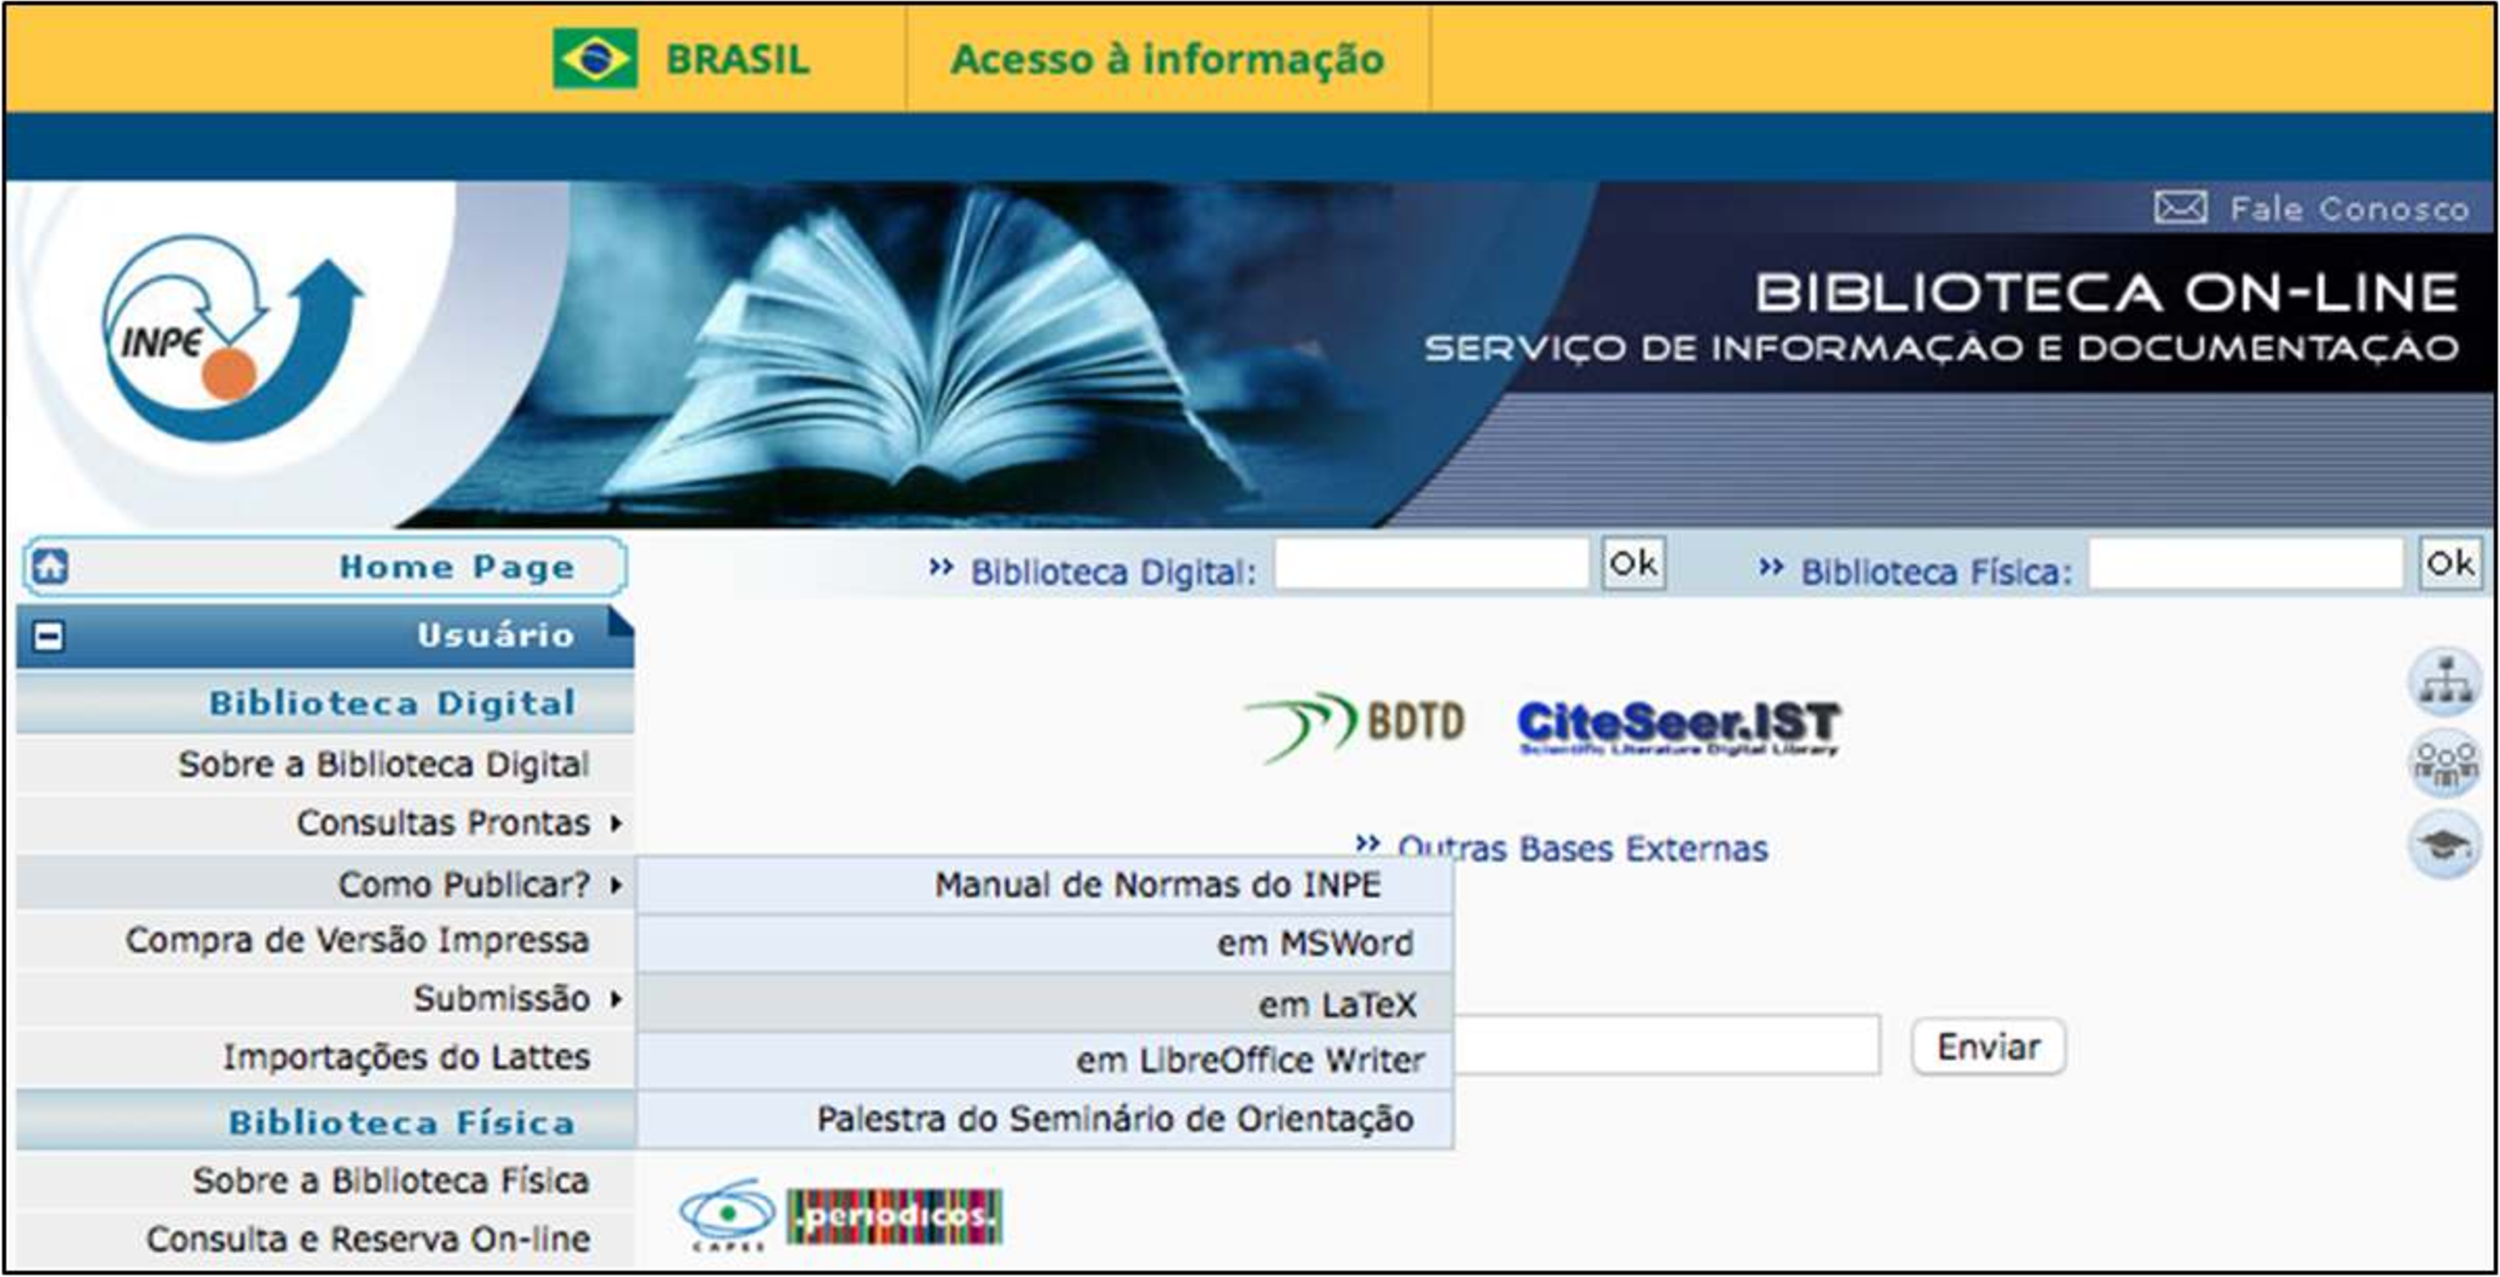
\includegraphics[scale=0.25]{./figs/biblio_pub_latex.pdf}
    \end{center}
\caption{Obtenção do estilo \LaTeX{} do INPE a partir do \textit{site} da Biblioteca do INPE.}
\end{figure}
\end{block}
\end{frame}

\subsection{Estrutura e Organização}

\begin{frame}[fragile]{Estrutura e Organização}
    \begin{block}{Arquivo {\tt archive.zip}}
        \vspace{1em}
        \begin{tcblisting}{colback=yellow!5,colframe=yellow!50!black,listing only,title=Descompactar o arquivo (Linux/MacOS),fonttitle=\small\bfseries,listing engine=minted,minted language=bash}
            unzip archive.zip
        \end{tcblisting}
        No \textit{Microsoft Windows}, basta clicar com o botão direito e clicar em ``Descompactar...''.
    \end{block}
\end{frame}

\begin{frame}{Estrutura e Organização}
\begin{figure}[H]
    \vspace{1em}
    \begin{center}
        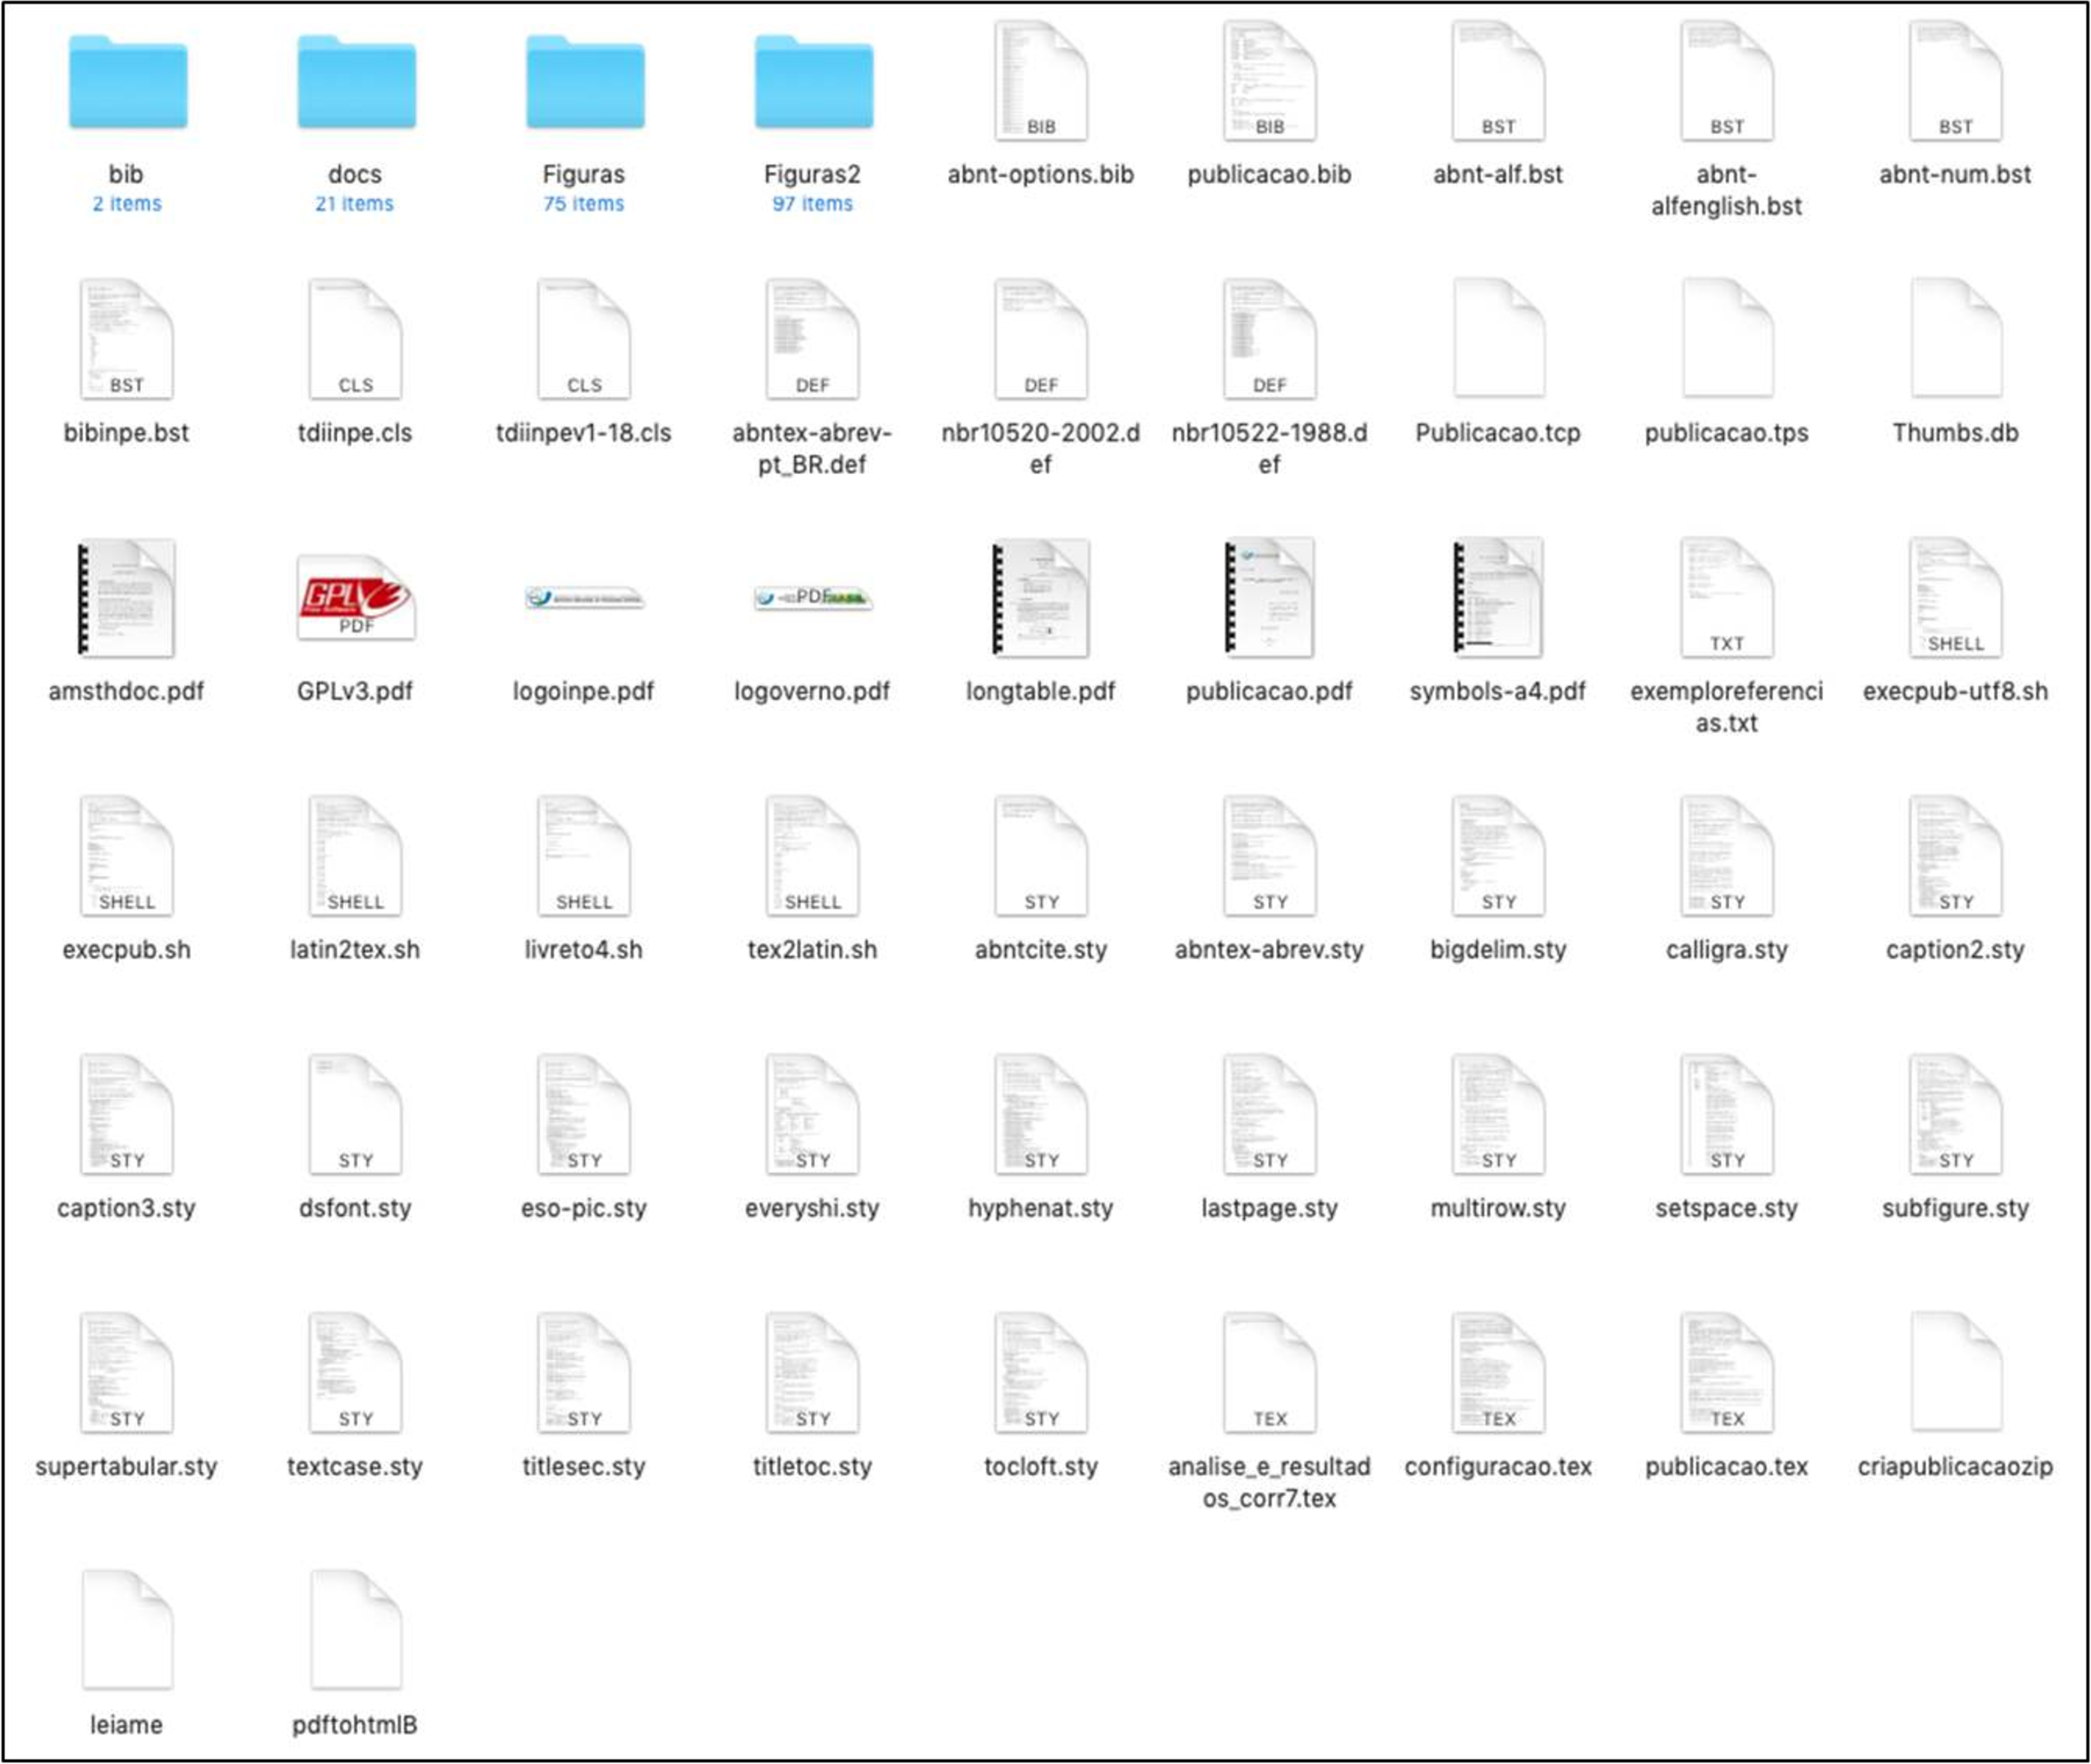
\includegraphics[scale=0.17]{./figs/estrutura_estilo_inpe.pdf}
    \end{center}
\caption{Estrutura e organização do estilo \LaTeX{} do INPE.}
\end{figure}
\end{frame}

\begin{frame}{Estrutura e Organização}
    \begin{multicols}{4}
    {\scriptsize
        \pause
        \textbf{Diretórios}
        \begin{itemize}[leftmargin=0pt, itemindent=0pt,labelwidth=15pt,labelsep=0pt, listparindent=0cm,align=left]
            \item bib/
            \item Figuras/
            \item docs/
        \end{itemize}
        \pause
        \textbf{Arquivos do Estilo}
        \begin{itemize}[leftmargin=0pt, itemindent=0pt,labelwidth=15pt,labelsep=0pt, listparindent=0cm,align=left]
            \color{blue}{\item leiame
            \item GPLv3.pdf
            \item CCBY.png
            \item CCBYNC.png
            \item CCBYNCND.png
            \item CCBYNCSA.png
            \item CCBYND.png
            \item CCBYSA.png
            \item logoverno.pdf
            \item logoinpe.pdf
            \item tdiinpe.cls}                                                        
            \pause
            \color{red}{\item abntex-abrev-pt\_BR.def      
            \item abntex-abrev.sty
            \item nbr10520-2002.def
            \item nbr10522-1988.def
            \item abnt-alf.bst
            \item abnt-alfenglish.bst
            \item bibinpe.bst
            \item eso-pic.sty
            \item abnt-num.bst
            \item abnt-options.bib
    		\item abntcite.sty}
        \end{itemize}
        \pause
    	\textbf{Outros Pacotes Fornecidos}
    	\begin{itemize}[leftmargin=0pt, itemindent=0pt,labelwidth=15pt,labelsep=0pt, listparindent=0cm,align=left]
            \item caption2.sty
            \item calligra.sty
            \item caption3.sty
    		\item hyphenat.sty
    		\item multirow.sty    
            \item dsfont.sty
    		\item supertabular.sty
    		\item tocloft.sty   
            \item setspace.sty
    		\item titlesec.sty   
            \item textcase.sty
    		\item lastpage.sty     
            \item bigdelim.sty
    		\item everyshi.sty 
            \item subfigure.sty
    		\item titletoc.sty
    	\end{itemize}
        \pause
    	\textbf{Arquivos de Configuração}
    	\begin{itemize}[leftmargin=0pt, itemindent=0pt,labelwidth=15pt,labelsep=0pt, listparindent=0cm,align=left]
    		\item configuracao.tex
    	\end{itemize}
        \pause
        \textbf{Arquivos de Documentos}
        \begin{itemize}[leftmargin=0pt, itemindent=0pt,labelwidth=15pt,labelsep=0pt, listparindent=0cm,align=left]
            \item publicacao.tex
        \end{itemize}
        \pause
        \textbf{\textit{Scripts}}
        \begin{itemize}[leftmargin=0pt, itemindent=0pt,labelwidth=15pt,labelsep=0pt, listparindent=0cm,align=left]
            \item tex2latin.sh
            \item criapublicacaozip
            \item latin2tex.sh
            \item pdftohtmlB
            \item livreto4.sh
            \item execpub.sh
        \end{itemize}
        \pause
        \textbf{Documento Final}
        \begin{itemize}[leftmargin=0pt, itemindent=0pt,labelwidth=15pt,labelsep=0pt, listparindent=0cm,align=left]
            \item publicacao.pdf
        \end{itemize}
    }
    \end{multicols}
\end{frame}

\begin{frame}{Estrutura e Organização}
    \begin{block}{\textit{Scripts} do estilo do INPE}
        \begin{itemize}[label=\textbullet]
            \pause
            \item \textbf{criapublicacaozip}: \textit{script} que empacota o documento final ({\tt publicacao.pdf}) para publicação;
            \pause
            \item \textbf{latin2tex.sh}: \textit{script} que converte acentos latinos para a marcação da linguagem \LaTeX{};
            \pause
            \item \textbf{tex2latin.sh}: \textit{script} que converte acentos com marcação \LaTeX{} para acentos latinos;
            \pause
            \item \textbf{pdftohtmlB}: converte um documento PDF em HTML;
            \pause
            \item \textbf{livreto4.sh}: gera um livreto de quatro folhas no formato A4;
            \pause
            \item \textbf{execpub.sh}: gera o documento de saída ({\tt publicacao.pdf}) utilizando o compilador \LaTeX{}. 
        \end{itemize}       
    \end{block}
\end{frame}

\subsection{Arquivos de Configuração}

\begin{frame}{Arquivos de Configuração}
    \begin{block}{Arquivos principais}
        \begin{itemize}[label=\textbullet]
            \item {\tt publicacao.tex}
            \item {\tt configuracao.tex}
        \end{itemize}
    \end{block}
\end{frame}

%\begin{frame}[plain,fragile]{}
%    \begin{tcblisting}{colback=yellow!5,colframe=yellow!50!black,listing only,title=Arquivo {\tt publicacao.tex},fonttitle=\bfseries,listing engine=minted,minted language=latex}
%        documentclass[
%        % PARA ESCOLHER O ESTILO TIRE O SIMBOLO (COMENTÁRIO)
%        ...
%        %PublicacaoDissOuTese,
%        %PublicacaoArtigoOuRelatorio,
%        %PublicacaoProposta, 
%        %PublicacaoLivro, 
%        %PublicacaoLivro,SemFormatacaoCapitulo,
%        english,portuguese, 
%        %portuguese,english, 
%        LogoINPE,
%        CCBYNC,
%        ]{tdiinpe}
%        ...
%    \end{tcblisting}  
%\end{frame}

\begin{frame}[plain,fragile]{}
    \begin{tcblisting}{
        theorem={Listing}{listings}{Arquivo {\tt publicacao.tex}}{lst:example1},
        title=Arquivo {\tt publicacao.tex},
        fonttitle=\small\bfseries,
        center,width=0.92\paperwidth,
        colback=yellow!5,colframe=yellow!50!black
        listing engine=minted,
        minted language=latex,
        minted options={%
            linenos,
            breaklines,
            autogobble,
            fontsize=\small,
            numbersep=2mm,
            baselinestretch=1},
        overlay={%
        \begin{tcbclipinterior}
            \fill[gray!25] (frame.south west) rectangle ([xshift=4mm]frame.north west);
        \end{tcbclipinterior}},
        breakable, enhanced, listing only}
        documentclass[
        % PARA ESCOLHER O ESTILO TIRE O SIMBOLO (COMENTÁRIO)
        %SemVinculoColorido,
        %SemFormatacaoCapitulo,
        %SemFolhaAprovacao,
        %SemImagens,
        %CitacaoNumerica, 
        %PublicacaoDissOuTese,
        %PublicacaoArtigoOuRelatorio,
        %PublicacaoProposta, 
        %PublicacaoLivro, 
        %PublicacaoLivro,SemFormatacaoCapitulo,
        english,portuguese, 
        %portuguese,english, 
        LogoINPE,
        CCBYNC,
        ]{tdiinpe}
        ...
    \end{tcblisting}
\end{frame}

\begin{frame}[plain,fragile]{}
    \begin{tcblisting}{
        theorem={Listing}{listings}{Arquivo {\tt publicacao.tex} (Continuação)}{lst:example1},
        title=Arquivo {\tt publicacao.tex} (Continuação),
        fonttitle=\small\bfseries,
        center,width=0.92\paperwidth,
        colback=yellow!5,colframe=yellow!50!black
        listing engine=minted,
        minted language=latex,
        minted options={%
            linenos,
            breaklines,
            autogobble,
            fontsize=\small,
            numbersep=2mm,
            baselinestretch=1},
        overlay={%
        \begin{tcbclipinterior}
            \fill[gray!25] (frame.south west) rectangle ([xshift=4mm]frame.north west);
        \end{tcbclipinterior}},
        breakable, enhanced, listing only}
        ...
        %\watermark{Revisão No. ##} 
        \usepackage{rotating}
        \usepackage{dsfont}
        \usepackage{comment}
        
        %%%%%%%%%%%%%%%%%%%CAPA%%%%%%%%%%%%%%%%%%%%%%%%%%%%%%%%
%\serieinpe{INPE-NNNNN-TDI/NNNN} %% n\~{a}o mais usado

\titulo{Escrever o t\'{i}tulo no idioma em que foi escrito a publicaç\~{a}o}
\title{Escrever o t\'{i}tulo em Ingl\^{e}s para publicaç\~{o}es escritas em Portugu\^{e}s e em Portugu\^{e}s para publicaç\~{o}es escritas em Ingl\^{e}s} %% 
\author{Nome Completo do Autor} %% coloque o nome do(s) autor(es)
\descriccao{Tese de Doutorado ou Dissertaç\~{a}o de Mestrado do Curso de P\'{o}s-Graduaç\~{a}o em Nome do Curso, orientada pelo(a) Dr(a). Nome do Orientador(a), aprovada em dd de m\^{e}s por extenso de aaaa.}
\repositorio{aa/bb/cc/dd} %% reposit\'{o}rio onde est\'{a} depositado este documento - na omiss\~{a}o, ser\'{a} preenchido pelo SID
\tipoDaPublicacao{TDI}	%% tipo da publicaç\~{a}o (NTC, RPQ, PRP, MAN, PUD, TDI, TAE e PRE) na aus\^{e}ncia do n\'{u}mero de s\'{e}rie INPE, caso contr\'{a}rio deixar vazio
\IBI{xx/yy} %% IBI (exemplo: J8LNKAN8PW/36CT2G2) quando existir, caso contr\'{a}rio o nome do reposit\'{o}rio onde est\'{a} depositado o documento

\date{AAAA}%ano da publicaç\~{a}o

%%%%%%%%%%%%%%%%%%%%%%%%%%VERSO DA CAPA%%%%%%%%%%%%%%%%%%%%%%%%%%%%%%%%%%%%%%%%%%%%%%%
\tituloverso{\vspace{-0.9cm}\textbf{\PublicadoPor:}}
\descriccaoverso{Instituto Nacional de Pesquisas Espaciais - INPE\\
Gabinete do Diretor (GB)\\
Serviço de Informaç\~{a}o e Documentaç\~{a}o (SID)\\
Caixa Postal 515 - CEP 12.245-970\\
S\~{a}o Jos\'{e} dos Campos - SP - Brasil\\
Tel.:(012) 3945-6923/6921\\
Fax: (012) 3945-6919\\
E-mail: {\url{pubtc@sid.inpe.br}}
}

\descriccaoversoA{\textbf{\ConselhoDeEditoracao:}\\
\textbf{\Presidente:}\\
Marciana Leite Ribeiro - Serviço de Informaç\~{a}o e Documentaç\~{a}o (SID)\\
\textbf{\Membros:}\\
Dr. Gerald Jean Francis Banon - Coordenaç\~{a}o Observaç\~{a}o da Terra (OBT)\\
Dr. Amauri Silva Montes - Coordenaç\~{a}o Engenharia e Tecnologia Espaciais (ETE)\\
Dr. Andr\'{e} de Castro Milone - Coordenaç\~{a}o Ci\^{e}ncias Espaciais e Atmosf\'{e}ricas (CEA)\\
Dr. Joaquim Jos\'{e} Barroso de Castro -  Centro de Tecnologias Espaciais (CTE)\\
Dr. Manoel Alonso Gan - Centro de Previs\~{a}o de Tempo e Estudos Clim\'{a}ticos (CPT)\\
Drª Maria do Carmo de Andrade Nono - Conselho de P\'{o}s-Graduaç\~{a}o\\
Dr. Pl\'{i}nio Carlos Alval\'{a} - Centro de Ci\^{e}ncia do Sistema Terrestre (CST)\\
\textbf{\BibliotecaDigital:}\\
Dr. Gerald Jean Francis Banon - Coordenaç\~{a}o de Observaç\~{a}o da Terra (OBT)\\
Clayton Martins Pereira - Serviço de Informaç\~{a}o e Documentaç\~{a}o (SID)\\
%Jefferson Andrade Ancelmo - Serviço de Informaç\~{a}o e Documentaç\~{a}o (SID)\\
%Simone A. Del-Ducca Barbedo - Serviço de Informaç\~{a}o e Documentaç\~{a}o (SID)\\
%Deicy Farabello - Centro de Previs\~{a}o de Tempo  e Estudos Clim\'{a}ticos (CPT)\\
\textbf{\RevisaoNormalizacaoDocumentaria:}\\
Simone Ang\'{e}lica Del Ducca Barbedo - Serviço de Informaç\~{a}o e Documentaç\~{a}o (SID) \\
%Maril\'{u}cia Santos Melo Cid - Serviço de Informaç\~{a}o e Documentaç\~{a}o (SID)\\
Yolanda Ribeiro da Silva Souza - Serviço de Informaç\~{a}o e Documentaç\~{a}o (SID)\\
\textbf{\EditoracaoEletronica:}\\
Marcelo de Castro Pazos - Serviço de Informaç\~{a}o e Documentaç\~{a}o (SID)\\
Andr\'{e} Luis Dias Fernandes - Serviço de Informaç\~{a}o e Documentaç\~{a}o (SID)\\
}

%%%%%%%%%%%%%%%%%%%FOLHA DE ROSTO

%%%%%%%%%%%%%%%FICHA CATALOGRÁFICA
%% NÃO PREENCHER - SERÁ PREENCHIDO PELO SID

\cutterFICHAC{Cutter}
\autorUltimoNomeFICHAC{Sobrenome, Nomes} %% exemplo: Fuckner, Marcus Andr\'{e}
\autorAbreviadoFICHAC {} %% N\~{a}o usado - deixar vazio
\tituloFICHAC{Titulo da publicaç\~{a}o}
\instituicaosigla{INPE}
\instituicaocidade{S\~{a}o Jos\'{e} dos Campos}
\paginasFICHAC{\pageref{numeroDePaginasDoPretexto} + \pageref{LastPage}} %% n\'{u}mero total de p\'{a}ginas
%\serieinpe{INPE-00000-TDI/0000} %% n\~{a}o mais usado
\palavraschaveFICHAC{1.~Palavra chave. 2.~Palavra chave 3.~Palavra chave. 4.~Palavra chave. 5.~Palavra chave  I.~\mbox{T\'{i}tulo}.} %% recomenda-se pelo menos 5 palavras-chaves - \mbox{} \'{e} para evitar hifenizaç\~{a}o 
\numeroCDUFICHAC{000.000} %% n\'{u}mero do CDU 

% Nota da ficha (para TD)
\tipoTD{Dissertaç\~{a}o ou Tese} % Dissertaç\~{a}o ou Tese
\cursoFA{Mestrado ou Doutorado em Nome do Curso}
\instituicaoDefesa{Instituto Nacional de Pesquisas Espaciais}
\anoDefesa{AAAA} % ano de defesa 
\nomeAtributoOrientadorFICHAC{Orientador}	% pode ser: Orientador, Orientadora ou Orientadores
\valorAtributoOrientadorFICHAC{Jos\'{e} da Silva} % nome(s) completo(s)

%%%%%%%%%%%%%%%FOLHA DE APROVAÇAO PELA BANCA EXAMINADORA
\tituloFA{\textbf{ATENÇÃO! A FOLHA DE APROVAÇÃO SERÁ INCLUIDA POSTERIORMENTE.}}
%\cursoFA{\textbf{}}
\candidatoOUcandidataFA{}
\dataAprovacaoFA{}
\membroA{}{}{}
\membroB{}{}{}
\membroC{}{}{}
\membroD{}{}{}
\membroE{}{}{}
\membroF{}{}{}
\membroG{}{}{}
\ifpdf

%%%%%%%%%%%%%%NÍVEL DE COMPRESSÃO {0 -- 9}
\pdfcompresslevel 9
\fi
%%% define em 80% a largura das figuras %%%
\newlength{\mylenfig} 
\setlength{\mylenfig}{0.8\textwidth}
%%%%%%%%%%%%%%%%%%%%%%%%%%%%%%%%%%%%%%%%%%%

%%%%%%%%%%%%%%COMANDOS PESSOAIS
\newcommand{\vetor}[1]{\mathit{\mathbf{#1}}} 
        
        \makeindex  
        ... 
        \marcaRegistrada{Informar aqui sobre marca registrada (a modificação desta linha deve ser feita no arquivo publicacao.tex).}
        \financiamento{Informar aqui sobre fontes financiadoras (a modificação desta linha deve ser feita no arquivo publicacao.tex).}
         
        \maketitle  
        ...
    \end{tcblisting}
\end{frame}

\begin{frame}[plain,fragile]{}
    \begin{tcblisting}{
        theorem={Listing}{listings}{Arquivo {\tt publicacao.tex} (Continuação)}{lst:example1},
        title=Arquivo {\tt publicacao.tex} (Continuação),
        fonttitle=\small\bfseries,
        center,width=0.92\paperwidth,
        colback=yellow!5,colframe=yellow!50!black
        listing engine=minted,
        minted language=latex,
        minted options={%
            linenos,
            breaklines,
            autogobble,
            fontsize=\small,
            numbersep=2mm,
            baselinestretch=1},
        overlay={%
        \begin{tcbclipinterior}
            \fill[gray!25] (frame.south west) rectangle ([xshift=4mm]frame.north west);
        \end{tcbclipinterior}},
        breakable, enhanced, listing only}
        ...
        % Comente as linhas opcionais abaixo caso não as deseje
        %%%%%%%%%%%%%%%%%%%%%%%%%%%%%%%%%%%%%%%%%%%%%%%%%%%%%%%%%%%%%%%%%%%%%%%%%%%%%%%%
% Epígrafe %% opcional

\begin{epigrafe} %% insira sua epígrafe abaixo; estilo livre

\hypertarget{estilo:epigrafe}{} %% uso para este Guia
 
\textit{\large``The language in which we express our ideas has a strong influence on our thought processes.''}

\vspace{1cm}

\hspace{4cm} \emph{\textsc{Donald Ervin Knuth}}\\\hspace{4cm} em \textsl{``Literate Programming''}, 1992

%For example, if \lstinline|\thinmskip = 3mu|, this makes \lstinline|\thickmskip = 6mu|. But if you also want to use \lstinline|\skip12| for horizontal glue, whether in math mode or not, the amount of skipping will be in points (e.g., 6pt). The rule is that glue in math mode varies with the size only when it is an \lstinline|\mskip|; when moving between an mskip and ordinary skip, the conversion factor \lstinline|1mu=1pt| is always used. The meaning of `\lstinline|\mskip\skip12|' and `\lstinline|\baselineskip=\the\thickmskip\lstinline|' should be clear.
%
%\vspace{1cm}
%
%\hspace{4cm} \emph{\textsc{Donald Ervin Knuth}}\\\hspace{4cm} em \textsl{``\TeX 82 -- Comparison with \TeX80''}

\end{epigrafe} % Opcional
        %%%%%%%%%%%%%%%%%%%%%%%%%%%%%%%%%%%%%%%%%%%%%%%%%%%%%%%%%%%%%%%%%%%%%%%%%%%%%%%%
% Dedicatória %% opcional

\begin{dedicatoria} %% insira sua dedicatória abaixo; estilo livre

\hypertarget{estilo:dedicatoria}{} %% uso para este Guia
 
%% use 'a meus' em vez de 'aos meus', isto é, não use o artigo definido com pronomes possessivos

\newcommand{\mytext}{A meus pais \textbf{Nicanor} e \textbf{Jaci}, à minha irmã \textbf{Luciana} e ao meu esposo \textbf{William}}

\begin{comment}
%%% sugestão de estilo
\ifcalligra %% fonte calligra presente nas versões mais novas do MiKTeX (>= 2.4)
  \calligra\Large \mytext %% exemplo usando estilo de fonte caligráfica, caso haja
\else
	\itshape\Large \mytext 
\fi
\end{comment}

	\itshape\Large \mytext 

\end{dedicatoria}
 % Opcional
        %%%%%%%%%%%%%%%%%%%%%%%%%%%%%%%%%%%%%%%%%%%%%%%%%%%%%%%%%%%%%%%%%%%%%%%%%%%%%%%%
% AGRADECIMENTOS %% opcional

\begin{agradecimentos}  %% insira abaixo seus agradecimentos

\hypertarget{estilo:agradecimentos}{} %% uso para este Guia
Agradecemos à MsC Andriana Susana Lopes de Oliveira Campanharo que gentilmente cedeu 
parte dos textos de sua dissertação para este estilo. O original de sua dissertação
encontra-se na Biblioteca Digital do INPE, no endereço \url {http://urlib.net/sid.inpe.br/MTC-m13@80/2006/11.07.12.37}.
Agradecemos também ao Dr. Gerald Jean Francis Banon pelo desenvolvimento e disponibilização deste estilo.
\end{agradecimentos}


 % Opcional
        %%%%%%%%%%%%%%%%%%%%%%%%%%%%%%%%%%%%%%%%%%%%%%%%%%%%%%%%%%%%%%%%%%%%%%%%%%%%%%%%
% RESUMO %% obrigatório

\begin{resumo}

%% neste arquivo resumo.tex
%% o texto do resumo e as palavras-chave têm que ser em Português para os documentos escritos em Português
%% o texto do resumo e as palavras-chave têm que ser em Inglês para os documentos escritos em Inglês
%% os nomes dos comandos \begin{resumo}, \end{resumo}, \palavraschave e \palavrachave não devem ser alterados

\hypertarget{estilo:resumo}{} %% uso para este Guia

%Neste trabalho é analisada a possível natureza caótica da turbulência atmosférica. As análises aqui realizadas, baseadas em dados de temperatura de alta resolução, obtidos pela campanha WETAMC do projeto LBA, sugerem a existência de um comportamento caótico de baixa dimensão na camada limite atmosférica. O atrator caótico correspondente possui uma dimensão de correlação de $D_{2}=3.50\pm0.05$. A presença de dinâmica caótica nos dados analisados é confirmada com a estimativa de um expoente de Lyapunov pequeno mas positivo, com valor $\lambda_{1}=0.050\pm0.002$. No entanto, esta dinâmica caótica de baixa dimensão está associada à presença das estruturas coerentes na camada limite atmosférica e não à turbulência atmosférica. Esta afirmação é evidenciada pelo processo de filtragem por wavelets utilizado nos dados experimentais estudados, que permite separar a contribuição da estruturas coerentes do sinal turbulento de fundo.

Este material apresenta a linguagem de marcação \LaTeX{} para a confecção de textos científicos, tendo como foco o estilo de publicações do INPE. São apresentados os aspectos históricos de formulação da linguagem e as motivações para o seu uso dentro do ambiente acadêmico. O objetivo principal do uso da linguagem é permitir que o usuário concentre-se na escrita do texto, no desenvolvimento das suas ideias sem ter que se preocupar com a determinação e o posicionamento dos diversos elementos estruturais de um documento. Não se trata, porém, de um curso de escrita científica, mas sim de um manual objetivo para a aplicação da linguagem de marcação \LaTeX{} utilizando, especialmente, o estilo de publicações do INPE. Ao consultar o conteúdo deste material, o usuário estará habilitado a aplicar a linguagem na elaboração e desenvolvimento dos seus trabalhos acadêmicos e científicos.

\palavraschave{%
	\palavrachave{\LaTeX{}}%
	\palavrachave{Escrita Científica}%
	\palavrachave{Linguagem de Marcação}%
}
 
\end{resumo} % Obrigatório
        %%%%%%%%%%%%%%%%%%%%%%%%%%%%%%%%%%%%%%%%%%%%%%%%%%%%%%%%%%%%%%%%%%%%%%%%%%%%%%%%
% ABSTRACT


\begin{abstract}

%% neste arquivo abstract.tex
%% o texto do resumo e as palavras-chave têm que ser em Inglês para os documentos escritos em Português
%% o texto do resumo e as palavras-chave têm que ser em Português para os documentos escritos em Inglês
%% os nomes dos comandos \begin{abstract}, \end{abstract}, \keywords e \palavrachave não devem ser alterados

\selectlanguage{english}	%% para os documentos escritos em Português
%\selectlanguage{portuguese}	%% para os documentos escritos em Inglês

\hypertarget{estilo:abstract}{} %% uso para este Guia

In this work the possible chaotic nature of the atmospheric turbulence is analysed. The analyses carried out here, based in data of high resolution temperature, obtained from the WETAMC campaign of the LBA project, suggest the existence of a low-dimension chaotic behavior in the atmospheric boundary layer. The corresponding chaotic attractor possess a correlation dimension of $D_{2}=3.50\pm0.05$. The presence of chaotic dynamics in the analysed data is confirmed with the estimate of a small Lyapunov exponent but positive, with value $\lambda_{1}=0.050\pm0.002$. However, this low-dimension chaotic dynamics is associated with the presence of the coherent structures in the atmospheric boundary layer and not to the atmospheric turbulence. This affirmation is evidenced by the process of filtering for wavelets used in the studied experimental data, that allow to separate the contribution of the coherent structures of the turbulent background signal. 

\keywords{%
	\palavrachave{Atmospheric turbulence}%
	\palavrachave{WETAMC campaign}%
	\palavrachave{LBA project}%
	\palavrachave{Chaotic behavior}%
	\palavrachave{Chaotic attractor}%
}

\selectlanguage{portuguese}	%% para os documentos escritos em Português
%\selectlanguage{english}	%% para os documentos escritos em Inglês

\end{abstract}
 % Obrigatório
        
        \includeListaFiguras % Obrigatório (mais de 3 figuras)
        \includeListaTabelas % Obrigatório (mais de 3 tabelas)
        
        %%%%%%%%%%%%%%%%%%%%%%%%%%%%%%%%%%%%%%%%%%%%%%%%%%%%%%%%%%%%%%%%%%%%%%%%%%%%%%%%
%abreviaturas e siglas  %% opcional, mas recomendado

\begin{abreviaturasesiglas}  %% insira abaixo suas abreviaturas conforme o modelo.

%% sigla (separador: &--&) significado (quebra de linha: \\)
\\
ABNT     &--& Associação Brasileira de Normas Técnicas \\
AMS      &--& American Meteorological Society \\
APT      &--& Advanced Packaging Tool \\
BASIC    &--& Beginner's All-purpose Symbolic Instruction Code \\
CC       &--& Creative Commons \\
CMYK     &--& Cyan Magenta Yellow Black \\
CTAN     &--& Comprehensive TeX Archive Network \\
DNF      &--& Dandified Yum \\
DVI      &--& DeVice-Independent \\
EPS      &--& Encapsulated PostScript \\
GIF      &--& Graphics Interchange Format \\
GNU      &--& GNU's Not UNIX \\
GUID     &--& Globally Unique Identifier \\
HTML     &--& Hypertext Markup Language \\
INPE     &--& Instituto Nacional de Pesquisas Especiais \\
ISO      &--& International Organization for Standardization \\
JPEG     &--& Joint Photographic Experts Group \\
\LaTeX{} &--& Lamport \TeX{} \\
Mac OS   &--& Macintosh Operating System \\
MIT      &--& Massachussets Institute of Technology \\
MWR      &--& Monthly Weather Review \\
PDF      &--& Portable Document Format \\
PNG      &--& Portable Network Graphics \\
POSIX    &--& Portable Operating System Interface \\
RGB      &--& Red Green Blue \\
SESID    &--& Serviço de Informação e Documentação \\
SVG      &--& Scalable Vector Graphics \\
SWL      &--& Subsistema Windows para Linux \\
%\TeX{}   &--& $\tau\epsilon\chi$ \\
UTF      &--& Unicode Transformation Format \\
VIM      &--& Vi Improved \\
WYSIWYG  &--& What You See Is What You Get \\
\end{abreviaturasesiglas} % Opcional
        \begin{simbolos}
\hypertarget{estilo:simbolos}{}
\\
a   &--& primeira contante \\
b   &--& segunda constante \\
$\rho$  &--& densidade de um fluido\\
$\nu$   &--& viscosidade cinemática\\
$R_{e}$  &--& número de Reynolds\\
$\alpha$  &--& constante de Kolmogorov\\
$k$ &--&  número de onda\\
$K$ &--&  curtose\\
$D_{0}$ &--& dimensão de contagem de caixas\\
$D_{1}$ &--& dimensão de informação\\
$D_{2}$  &--& dimensão de correlação\\
$\lambda_{1}$  &--& expoente de Lyapunov dominante\\
\end{simbolos}
 % Opcional
        
        \includeSumario % Obrigatório
        \inicioIntroducao % Não altere este comando
        ...
    \end{tcblisting}
\end{frame}

\begin{frame}[plain,fragile]{}
    \begin{tcblisting}{
        theorem={Listing}{listings}{Arquivo {\tt publicacao.tex} (Continuação)}{lst:example1},
        title=Arquivo {\tt publicacao.tex} (Continuação),
        fonttitle=\small\bfseries,
        center,width=0.92\paperwidth,
        colback=yellow!5,colframe=yellow!50!black
        listing engine=minted,
        minted language=latex,
        minted options={%
            linenos,
            breaklines,
            autogobble,
            fontsize=\small,
            numbersep=2mm,
            baselinestretch=1},
        overlay={%
        \begin{tcbclipinterior}
            \fill[gray!25] (frame.south west) rectangle ([xshift=4mm]frame.north west);
        \end{tcbclipinterior}},
        breakable, enhanced, listing only}
    ...
    %%%%%%%%%%%%%%%%%%%%%%%%%%%%%%%%%%%%%%%%%%%%%%%%%%%%%%%%%%%%%%%%%%%%%%%%%%%%%%%

\chapter{INTRODUÇÃO}

A complexidade da turbulência tem atraído a atenção de naturalistas, filósofos, e poetas durante vários séculos. Talvez o primeiro esboço de um fluxo turbulento, capturando detalhes com vários graus de realismo, tenha sido feito ainda no século XV por Leonardo da Vinci~\cite{sreenivasan/99}. Desde então, estudos científicos intensos em turbulência têm sido realizados, porém os resultados obtidos ainda não têm recompensado os grandes esforços empregados. Diversos modelos propostos ao longo do tempo, que incluem aqueles introduzidos por Kolmogorov e Landau deixam a desejar na descrição, explicação e predição do movimento turbulento~\cite{ruelle/91}. Conseqüentemente, a turbulência, durante o último século, foi considerada um dos problemas mais ``intratáveis'' da Física Clássica. Em resposta a essas dificuldades, novos modelos para o problema surgiram recentemente, influenciados pelo advento da teoria do caos, em particular através da caracterização via ``atratores caóticos''~\cite{ruelltak/71} 

O artigo clássico de \citeonline{lor/63} foi um dos primeiros trabalhos a descrever movimentos caóticos sobre um atrator de baixa dimensão. Tais movimentos são caracterizados por uma instabilidade intrínseca devido à sensibilidade do sistema às variações de suas condições iniciais. Como conseqüência, trajetórias de pontos inicialmente muito próximos separam-se, em média, exponencialmente ao longo do tempo no espaço de fase. É bastante surpreendente que um sistema dinâmico de apenas três dimensões, ou seja, descrito por três equações diferenciais ordinárias de primeira ordem, exiba movimentos surpreendentemente complexos que se assemelham, a primeira vista, a uma evolução aleatória. Desde que Lorenz introduziu seu modelo como uma aproximação da dinâmica de uma camada de fluido convectiva, conjectura-se que a atmosfera possa ter um intrínseco limite de previsibilidade e que a dinâmica atmosférica possa ser governada por atratores caóticos~\cite{weber/95}. 

Diversos estudos confirmam a presença de atratores caóticos associados a situações específicas, a partir de séries temporais em diferentes áreas. Porém, a existência ou não desses atratores ainda é um tema controverso. Atratores caóticos de baixa dimensão têm sido encontrados em trajetórias de ciclones tropicais~\cite{fraedrichandleslie/89}, em séries temporais marítimas~\cite{fraedrich/86,nicolis/84}, como também em séries temporais relacionadas ao fenômeno El Niño~\cite{goberelnino/92}. Atratores similares foram também encontrados na camada limite atmosférica a partir de séries temporais de pressão de superfície~\cite{fraedrich/86}, como também em séries temporais de temperatura, velocidade e umidade~\cite{xin/01,jaramillo/93,gallego/01,tiong/93}. Ainda, atratores de alta dimensão têm sido encontrados por \citeonline{grass/86} a partir de séries marítimas. Por outro lado, nenhum indício de um atrator foi encontrado nas análises realizadas por \citeonline{weber/95} com base em séries temporais turbulentas da velocidade do vento. Aliás, \citeonline{loratrat/91} afirma que não há razão alguma para acreditar que um sistema dinâmico complexo, como o clima, possua um atrator caótico de baixa dimensão associado. Ele conjecturou que a dinâmica caótica de baixa dimensão obtida por muitos autores, com base em séries temporais climáticas, está relacionada a existência de um conjunto de subsistemas de baixa dimensão ``fracamente'' acoplados ao sistema - clima.

A identificação de uma dinâmica caótica de baixa dimensão em escoamentos turbulentos na atmosfera tem permitido, se não conclusões definitivas, uma interpretação alternativa dos processos turbulentos, onde as estruturas dissipativas coerentes desempenham um papel relevante. Fisicamente, tais estruturas estão presentes nas grandes escalas do escoamento e podem agir como objetos rígidos descritos com poucos graus de liberdade. Desta forma, a detecção experimental de uma dinâmica de baixa dimensão pode estar relacionada não ao fenômeno da turbulência ``per se'', mas devido à existência de estruturas coerentes na atmosfera, como de certa forma intuído por \citeonline{loratrat/91}. Sob essa perspectiva, a complexidade da atmosfera que, a priori, deveria ser representada por um sistema dinâmico de alta dimensão, pode ``conter'' um ou mais atratores caóticos de baixa dimensão acoplados entre si.

%Contudo, é importante destacar que a compreensão física e matemática da \textit{turbulência completamente desenvolvida} como um fenômeno de alta dimensão, embora seja ainda incompleta, está em discordância com a figura de uma dinâmica de baixa dimensão que pode descrever vários aspectos da chamada \textit{turbulência fraca}~\cite{weber/95}. 

Estudos demonstram que a presença de estruturas coerentes em escoamentos turbulentos pode ser responsável, em média, por $40\%$ de todo o calor turbulento e fluxos de momento~\cite{lu/94}. Sob condições convectivas, elas são reconhecidas em séries temporais de flutuações de temperatura com uma gradual elevação da temperatura, seguida por uma súbita queda. Sob condições estáveis, este padrão se inverte e uma gradual queda é seguida por uma súbita elevação~\cite{oliver/02}. Nestas duas condições, a estrutura coerente é do tipo ``rampa''. 

A teoria de sistemas dinâmicos tem fornecido novas ferramentas para a análise de séries temporais estacionárias obtidas em experimentos, ou seja, com base na medida de um único observável $x(t_{i}),i=1,2,3,\ldots$. Pode até ser a única variável independente disponível associada ao sistema. Ou seja, é possível definir um espaço de fase que capture a dinâmica do sistema em uma estrutura geométrica imersa nesse espaço. O conjunto geométrico imerso é chamado \textit{atrator reconstruído} e ele é topologicamente equivalente ao atrator que seria produzido pela evolução do sistema dinâmico de equações, caso as mesmas fossem conhecidas. Reconstruída a dinâmica, a caracterização dos atratores pode ser feita por uma abordagem métrica. Esta abordagem, invariante por mudança de sistema de coordenadas, efetiva-se segundo uma \textit{caracterização dinâmica} ou então \textit{estático-estatística}. Na caracterização dinâmica obtém-se informações a respeito da taxa de expansão de trajetórias inicialmente próximas via expoentes de Lyapunov~\cite{wolf/85,eckrue/86,sanosawada/85} ou da taxa de produção de informação no sistema via entropia de Kolmogorov-Sinai~\cite{ruelleentrop/89}. Na caracterização estático-estatística, obtém-se informações sobre a estrutura local dos atratores, que se caóticos, serão, salvo raras exceções, caracterizados por uma medida fractal, que pode ser analisada através das dimensões generalizadas~\cite{grassproca/83}.

Existe à disposição uma grande variedade de algoritmos para a caracterização de caoticidade em baixa dimensão de sinais experimentais. Esses algoritmos, longe de constituir um corpo preciso, envolvendo na sua aplicação aspectos ainda não totalmente elucidados e estimativas de erro aparentemente otimistas, incluem procedimentos para a obtenção do espectro de expoentes de Lyapunov, da entropia de Kolmogorov-Sinai, da dimensão de correlação, etc. Ligada à caracterização de caos está a questão da redução de ruído e da reconstrução da dinâmica, problemas ainda não completamete resolvidos na análise de sinais experimentais~\cite{aguirre/00}. 

De modo geral, o objetivo deste trabalho é investigar a possível natureza caótica da turbulência na camada limite atmosférica, no interior e acima da copa da floresta Amazônica. Mais especificamente, deseja-se: (i) determinar se o conjunto de séries temporais em estudo inclui componentes com características de dinâmica caótica, que podem ser descritas (individualmente) por um sistema determinístico de baixa dimensão; (ii) compreender o papel das estruturas coerentes do tipo rampa na possível natureza caótica da turbulência sobre a copa da floresta Amazônica. Espera-se que os resultados aqui obtidos permitam elucidar a conjectura de \citeonline{loratrat/91}, partindo do pressuposto que os subsistemas atmosféricos de baixa dimensão, postulados por este autor, sejam de fato estruturas coerentes. Paralelamente, procura-se avaliar o desempenho de diversas ferramentas computacionais de caracterização de dinâmica caótica de baixa dimensão, na análise de séries temporais experimentais longas e contaminadas com ruído. \cite{sousa:2004},

Neste trabalho, foram utilizados dados turbulentos de temperatura e velocidade do vento, obtidos pela campanha WETAMC (Campanha de Mesoescala Atmosférica na Estação Úmida) do projeto LBA (Experimento de Grande Escala de Interação Biosfera-Atmosfera na Amazônia), amostrados a $60$ Hz, com duração de $30$ minutos. As medidas foram feitas com o auxílio de uma torre micrometeorológica de $66$ m de altura, simultaneamente em três diferentes alturas: Nível Superior ($66$ m - acima da copa); Nível Médio ($45$ m -  no topo da copa); e Nível Inferior ($21$ m - abaixo da copa). Dois períodos de medidas distintos foram selecionados: às 12 horas, quando a copa da floresta é aquecida pelo sol e o topo da copa é mais quente que os arredores, e assim a região acima da copa é instável; e às 23 horas, quando as condições são opostas, e a região acima da copa é estável~\cite{Ramos/04}.

%Os capítulos restantes desta dissertação estão organizados da seguinte maneira:
%\begin{itemize}
%\item{Capítulo 2}: A Seção~\ref{seccaos} aborda, por meio de sistemas-paradigma de comportamento caótico como o Mapa Logístico e as Equações de Lorenz, as principais características apresentadas por sistemas dinâmicos não-lineares caóticos. A Seção~\ref{secturb} é destinada, em grande parte, à descrição fenomenológica da turbulência. São ainda apresentadas alguns temas de grande relevância no estudo da turbulência, como o fenômeno da intermitência e as estruturas coerentes. Finalmente, a Seção~\ref{seccaosurb} expõe uma perspectiva adicional para a compreensão do fenômeno turbulento com base na teoria de sistemas dinâmicos, mais especificamente por meio de atratores caóticos~\cite{ruelltak/71}.
%\item{Capítulo 3}: Neste capítulo é feita uma descrição detalhada dos métodos e dos algoritmos disponíveis para a caracterização de caos determinístico presente em séries temporais experimentais. O tema é bastante extenso e especializado; como conseqüência, tal descrição será focada nos procedimentos mais utilizados para a reconstrução da dinâmica, para o cálculo de dimensão de atratores e do espectro de expoentes de Lyapunov. São abordados alguns problemas e limitações, do ponto de vista numérico, associados aos algoritmos utilizados, como também as dificuldades encontradas no tratamento de sinais experimentais. 
%\item{Capítulo 4}: Neste capítulo é realizada uma breve descrição dos dados coletados pela campanha WETAMC do projeto LBA, bem como do sítio experimental.
%\item{Capítulo 5}: Neste capítulo são aplicadas diversas ferramentas (descritas no Capítulo~\ref{caputiltecnicas}) nas séries temporais em estudo, em busca de atratores caóticos de baixa dimensão na camada limite atmosférica.
%\item{Capítulo 6}: Com base nas análises realizadas no Capítulo~\ref{capanaliseseresults}, neste capítulo serão apresentadas as conclusões obtidas, como também algumas sugestões para trabalhos futuros.
%\end{itemize}

 % 1o capítulo
    %%%%%%%%%%%%%%%%%%%%%%%%%%%%%%%%%%%%%%%%%%%%%%%%%%%%%%%%%%%%%%%%%%%%%%%%%%%%%%%%


%\chapter{SISTEMAS DIN�MICOS CA�TICOS E TURBUL�NCIA}  
%\label{caprevibiblio}
%
%Este cap�tulo aborda as principais caracter�sticas apresentadas por sistemas din�micos n�o-lineares ca�ticos. S�o ainda apresentadas as caracter�sticas gerais da turbul�ncia, como tamb�m alguns temas de grande relev�ncia nesta �rea, como o fen�meno da intermit�ncia e as estruturas coerentes. Finalmente, � exposta uma perspectiva adicional para a compreens�o do fen�meno turbulento com base na teoria de sistemas din�micos, mais especificamente por meio de atratores ca�ticos.
%
%\section{Sistemas Din�micos Ca�ticos}
%\label{seccaos}
%
%\subsection{Introdu��o}
%
%O estudo de modelos lineares criou paradigmas que se enraizaram  na tradi��o hist�rica. O determinismo estrito � um bom exemplo disto e pode ser bem representado pelo pensamento de Laplace: ``Devemos ver o estado presente do universo como o efeito do seu estado anterior, e como a causa daquele que vir�. Uma intelig�ncia que, em qualquer instante dado, soubesse todas as for�as pela qual o mundo natural se move e a posi��o de cada uma de suas partes componentes, e que tivesse tamb�m a capacidade de submeter todos estes dados � an�lise matem�tica, poderia englobar na mesma f�rmula os movimentos dos maiores objetos do universo e �queles dos menores �tomos: nada seria incerto para ele, e o futuro, assim como o passado, estaria presente diante de seus olhos''~\cite{gleick/87}.
%
%No final do s�culo XIX, Poincar� estudava o problema da din�mica de tr�s corpos, quando concluiu que o acaso deveria se contrapor ao determinismo estrito de Laplace: ``Uma causa muito diminuta, que nos escapa, determina um efeito consider�vel, que n�o podemos deixar de ver, e ent�o dizemos que este efeito � devido ao acaso. Se pud�ssemos conhecer exatamente as leis da natureza e a situa��o do universo no instante inicial, ser�amos capazes de prever exatamente a situa��o deste mesmo universo no instante subseq�ente. Mas mesmo quando as leis naturais j� n�o tivessem mais segredo para n�s, s� poder�amos conhecer a situa��o inicial aproximadamente. Se isto nos permite antecipar a situa��o subseq�ente com o mesmo grau de aproxima��o, ficamos satisfeitos, dizemos que o fen�meno foi previsto, que � governado por leis. Mas nem sempre isto ocorre: pode acontecer que diferen�as m�nimas nas condi��es iniciais produzam diferen�as muito grandes no fen�meno final: um erro m�nimo nas primeiras produziria um erro enorme neste �ltimo. A previs�o torna-se imposs�vel e temos o fen�meno do acaso''~\cite{gleick/87}.
%
%Apesar da clara vis�o de Poincar� a respeito da imprevisibilidade em alguns sistemas, foi s� em $1963$, quando Lorenz desenvolvia estudos sobre problemas atmosf�ricos, que se retomou a id�ia do acaso na \textit{an�lise de sistemas f�sicos de baixa dimens�o}. Contando com o aux�lio de um computador, Lorenz observou que uma pequena varia��o nas condi��es iniciais poderia acarretar grandes diferen�as na evolu��o do sistema~\cite{lor/63}. Este fen�meno ficou conhecido como efeito borboleta, como uma alus�o de que se uma borboleta batesse suas asas em algum lugar do planeta, poderia alterar a resposta de um sistema f�sico do outro lado da Terra. Tratava-se de um sistema totalmente determin�stico cujos resultados poderiam ser imprevis�veis se as condi��es de medida n�o pudessem ser determinadas com precis�o infinita. Iniciava-se o moderno estudo do caos, cujas id�ias b�sicas haviam sido lan�adas por Poincar�. 
%
%\subsection{Sistemas din�micos}
%
%Um \textit{sistema din�mico} � um sistema que evolui a cada instante de acordo com um conjunto de regras fixas que determinam como um estado do sistema se altera para um outro. Dois tipos principais de sistemas din�micos s�o encontrados em aplica��es: aqueles nos quais a vari�vel tempo � cont�nua ($t\in \mathds{R}$) e aqueles nos quais a vari�vel tempo � discreta ($t\in \mathds{N}$).
%
%Um \textit{sistema din�mico cont�nuo} pode ser descrito por equa��es diferenciais ordin�rias (EDO's) ou parciais (EDP's). Para o caso de uma ou mais EDO's, tal sistema assume a forma
%\begin{equation}
%\begin{array}{rcl} d\vec{x}(t)/dt & = & \vec{f}_{\mu}(\vec{x}(t)) \\ 
%                   \vec{x}(0) & = & \vec{x}_{0} \\
%\end{array}
%\label{eqedo}
%\end{equation}
%enquanto um \textit{sistema din�mico discreto} pode ser representado como a itera��o de uma ou mais fun��es, isto �
%\begin{equation}
%\vec{x}_{n+1} = \vec{f}_{\mu}(\vec{x}_{n})
%\label{eqmapa}
%\end{equation}
%onde $\vec{x}\in \mathds{R}^{m}$ corresponde ao vetor de estados do sistema, $\mu$ � definido como um \textit{par�metro de controle} do sistema e $\vec{x}(0)$ � o vetor de condi��es iniciais das vari�veis de estado do sistema din�mico. 
%
%Se $\vec{f}_{\mu}$ � constitu�do de $m$ fun��es cont�nuas lineares, o sistema din�mico � linear; caso contr�rio, o sistema din�mico � n�o-linear. Se $\vec{f}_{\mu}$ n�o depende explicitamente do tempo $t$, o sistema din�mico � aut�nomo; caso contr�rio o sistema � n�o-aut�nomo.
%
%O conjunto dos valores assumidos pelas vari�veis de estado ao longo do tempo, a partir da condi��o inicial $\vec{x}(0)$, � chamada de \textit{trajet�ria} ou \textit{�rbita} do sistema din�mico. As trajet�rias descritas pelas vari�veis de estado de um sistema din�mico s�o usualmente representadas em um espa�o euclidiano $\mathds{R}^{m}$, que neste contexto � chamado de \textit{espa�o de estados} ou ainda \textit{espa�o de fase}, sendo $m$ a dimens�o do sistema.
%
%
%\subsection{Caos em sistemas din�micos n�o-lineares}
%
%Desde a constata��o feita por Poincar� de que sistemas din�micos podem exibir comportamentos de extrema complexidade, uma s�rie de novos conceitos e ferramentas matem�ticas t�m sido desenvolvidos com sucesso, incluindo a abordagem qualitativa do fen�meno din�mico n�o-linear. Sobretudo, com o advento de sistemas de computa��o mais poderosos, � que o processo investigativo se acelerou, penetrando mais profundamente nas �reas da f�sica te�rica e da matem�tica computacional.
%
%Desde ent�o, in�meros pesquisadores passaram a analisar diferentes sistemas din�micos da forma (\ref{eqedo}) ou (\ref{eqmapa}). \citeonline{may/76}, por exemplo, tratou de um sistema din�mico relacionado com o crescimento populacional. Este trabalho abordou o \textit{mapa log�stico} para o qual avalia a popula��o $x$ no ano $n+1$ a partir da popula��o do ano anterior, ou seja,
%\begin{equation}
%x_{n+1}=\lambda x_{n}\left(x_{n}-1\right)
%\label{equalogis1}
%\end{equation}
%
%Este mapa � um sistema din�mico aut�nomo, discreto e unidimensional, isto �, caracterizado por uma �nica vari�vel de estado $x\in \mathds{R}$. O par�metro $\lambda$ define o tipo de resposta do sistema, ou seja, a itera��o do mapa (\ref{equalogis1}) para diferentes valores de $\lambda$ pode conduzir � solu��es est�veis, peri�dicas ou irregulares, como as apresentadas na Figura~\ref{figuralogis}. Em $(a)$, observa-se uma solu��o est�vel. Em $(b)$ e $(c)$, t�m-se solu��es peri�dicas de per�odos $2$ e $4$ respectivamente. J� em $(d)$, observa-se uma seq��ncia determin�stica e aperi�dica, caracter�stica de \textit{sistemas ca�ticos}.
%
%\begin{figure}[ht]
%\centering \resizebox{15cm}{!}{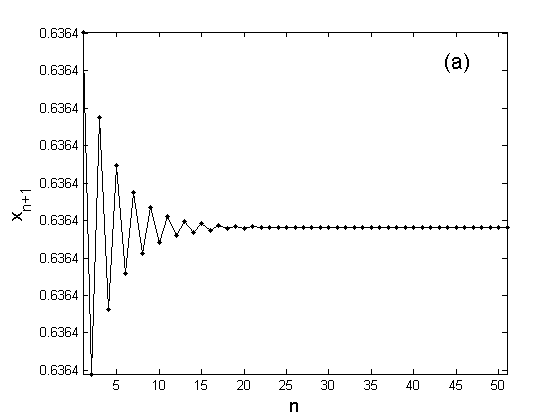
\includegraphics{docs/figs/logistico1.png}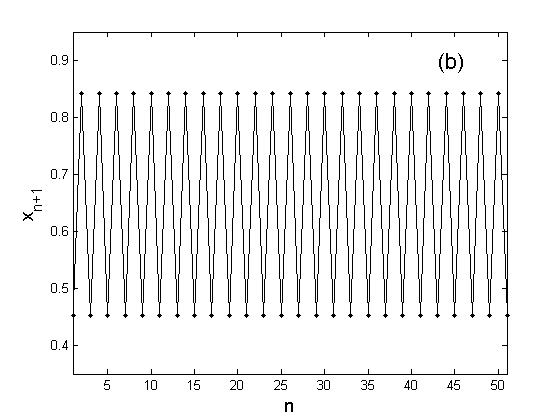
\includegraphics{docs/figs/logistico2.png}}\\ \resizebox{15cm}{!}{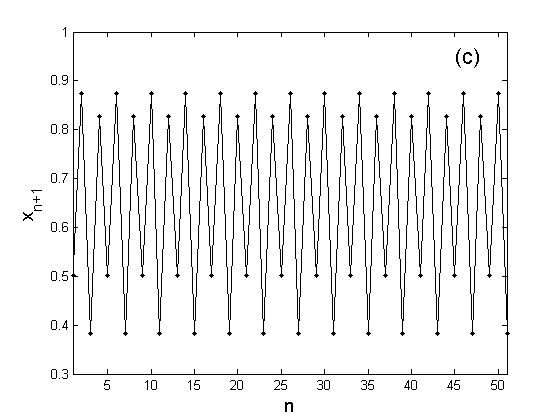
\includegraphics{docs/figs/logistico3.png} 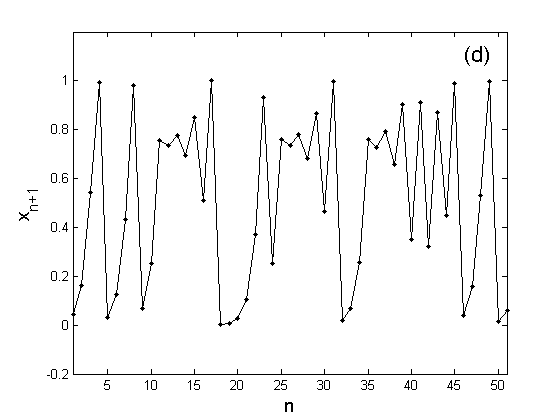
\includegraphics{docs/figs/logistico4.png}}
%\caption{S�ries temporais obtidas a partir da itera��o do mapa~(\ref{equalogis1}) com condi��o inicial fixa $x_{0}=0.01$ e para valores de $\lambda$ dados, respectivamente por $2.75$, $3.4$, $3.5$ e $4.0$.}
%\label{figuralogis}
%\end{figure}
%
%O mapa log�stico tamb�m evidencia outra caracter�stica dos sistemas ca�ticos: a \textit{imprevisibilidade}, ou seja, o conhecimento do valor aproximado do estado do sistema n�o permite predizer, de maneira imediata, sua evolu��o posterior para qualquer tempo futuro. Este comportamento est� associado � \textit{sensibilidade �s varia��es nas condi��es iniciais} e ao fato de n�o se conseguir obter com precis�o infinita o valor real do estado. Para o Sistema~(\ref{equalogis1}) valores muito pr�ximos de uma condi��o inicial $x_0$ conduzem, ap�s algumas poucas itera��es, a �rbitas completamente distintas, conforme pode ser observado na Figura~\ref{figuralogis2}.
%
%\begin{figure}[ht]
%\centering
%\resizebox{15cm}{!}{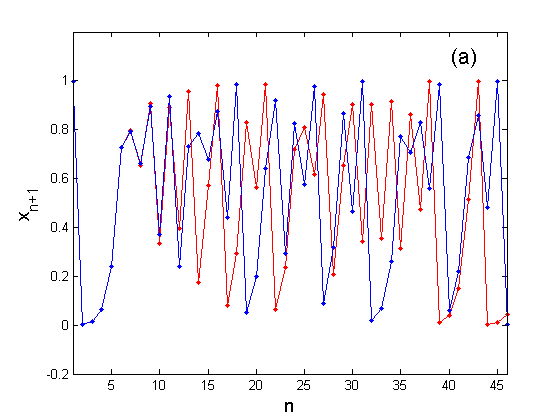
\includegraphics{docs/figs/logisticoci.png}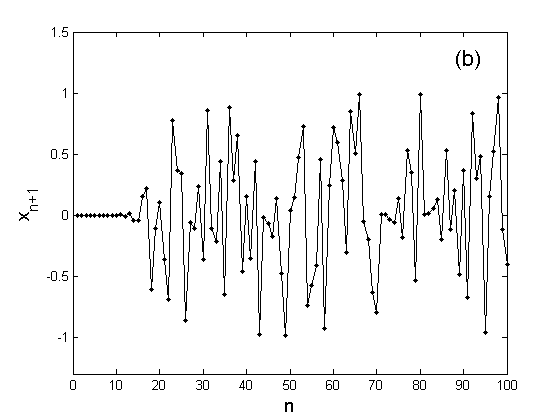
\includegraphics{docs/figs/logisticocidiff.png}}
%\caption{(a) S�ries temporais obtidas pela itera��o do mapa~(\ref{equalogis1}) para valores muito pr�ximos de $x_0$. A curva em azul corresponde � �rbita gerada com condi��o inicial $x_{0}=0.01$, enquanto que a curva em vermelho corresponde � �rbita gerada com condi��o inicial $x_{0}=0.010001$. (b) as diferen�as associadas �s duas �rbitas.}
%\label{figuralogis2}
%\end{figure}
%
%As trajet�rias ou �rbitas de um sistema ca�tico oscilam confinados em uma regi�o limitada do espa�o de estados, sem entretanto, apresentar periodicidade~\cite{alligood/97}. No interior desta regi�o, as vari�veis de estado exibem valores correspondentes a pontos no espa�o de fase para os quais as trajet�rias ca�ticas, iniciando em um n�mero significativo de condi��es iniciais, passam arbitrariamente pr�ximas, infinitas vezes, � medida que o sistema evolui no tempo. Isto �, uma vez iniciada a evolu��o do sistema, sua trajet�ria � \textit{atra�da} para um sub-conjunto de pontos do espa�o de fase, conhecido como \textit{atrator ca�tico}, e ali permanece percorrendo este sub-conjunto indefinidamente. O conjunto de todas as condi��es iniciais que converge para o atrator ca�tico � chamado \textit{bacia de atra��o} do atrator~\cite{alligood/97}.
%
%Se a estrutura geom�trica criada por estados assint�ticos das trajet�rias for um fractal, este � denominado atrator estranho. Atratores ca�ticos apenas ocorrem em sistemas dissipativos. Sobre este atrator, a din�mica � caracterizada por \textit{esticamentos} e \textit{dobras}; o primeiro fen�meno � respons�vel pela diverg�ncia de trajet�rias pr�ximas e o �ltimo � respons�vel pela contra��o da din�mica para uma regi�o finita em um subespa�o de dimens�o $\leq m$.  Em contraste com sistemas n�o-ca�ticos que possuem atratores de dimens�o inteira como pontos atrativos (que geram solu��es estacion�rias) e ciclos limites (que produzem solu��es peri�dicas), sistemas ca�ticos podem estar associados a atratores ca�ticos caracterizados por uma dimens�o n�o-inteira $d$. Esta dimens�o � uma propriedade do atrator, independentemente de uma trajet�ria em particular.
%
%Segundo \citeonline{ruelle/91} atratores ca�ticos que apresentam o fen�meno da \textit{sensibilidade �s varia��es nas condi��es iniciais}, correspondem � excita��o de um n�mero finito de graus de liberdade e embora tais atratores possuam dimens�o finita, a an�lise em termos de freq��ncias temporais revela um \textit{espectro cont�nuo de freq��ncias}. 
%
%O mapa de H�non � um exemplo de sistema din�mico discreto, que apresenta um atrator ca�tico em sua din�mica. Este mapa � descrito pelas equa��es 
%\begin{equation}
%\begin{array}{lcl} x_{n+1} & = & 1-ax_{n}^2+y_{n} \\ 
%                   y_{n+1} & = & bx_{n} \\
%\end{array}
%\label{eqhenon}
%\end{equation}
%sendo $a$ e $b$ par�metros do mapa. Para valores de $a=1.4$ e $b=0.3$, este sistema apresenta um comportamento irregular e aperi�dico que se desenvolve em um atrator ca�tico e estranho. O atrator de H�non e uma seq��ncia de sua amplia��o s�o mostrados na Figura~\ref{figurahenonsimilar}. A dimens�o fractal~\cite{mandelbrot/82} associada a esse atrator � de $1.265$, sendo evidente seu car�ter auto-similar - caracter�stica t�pica de atratores estranhos~\cite{alligood/97}.
%
%\begin{figure}[ht]
%\centering
%\resizebox{15cm}{!}{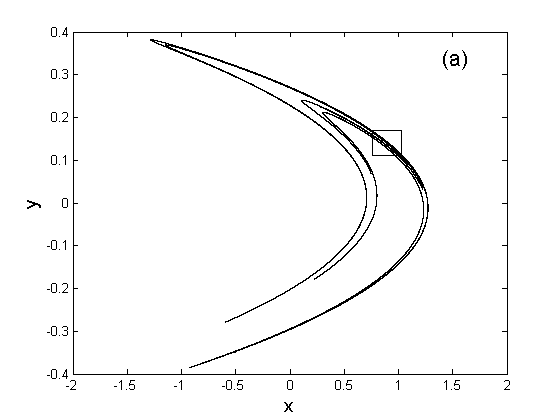
\includegraphics{docs/figs/henon.png}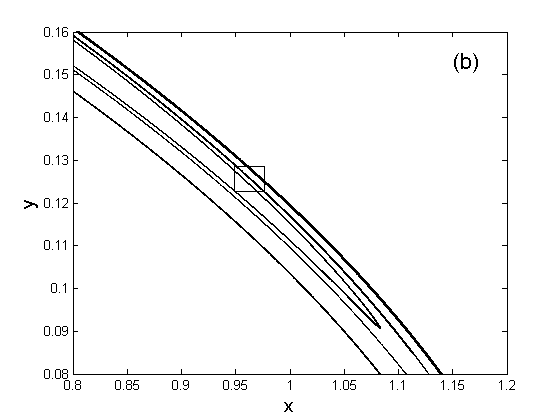
\includegraphics{docs/figs/henonamp1.png}}\\ \resizebox{15cm}{!}{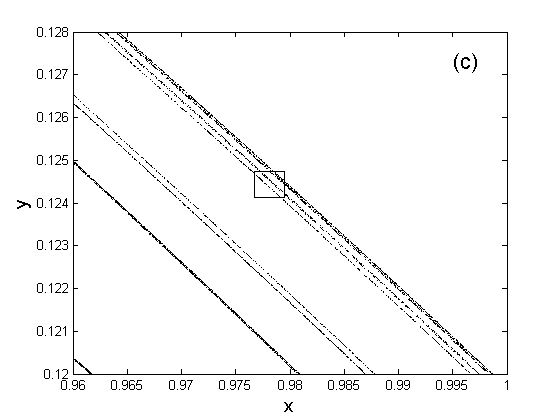
\includegraphics{docs/figs/henonamp2.png} 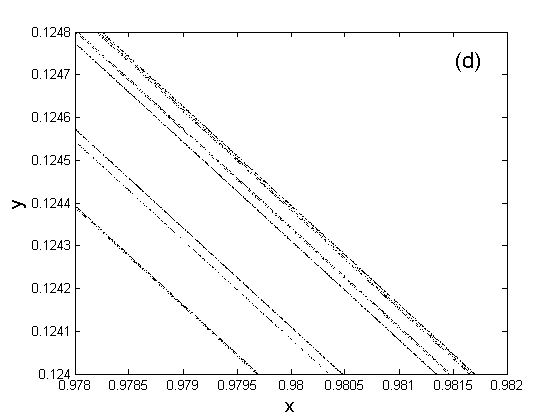
\includegraphics{docs/figs/henonamp3.png}}
%\caption{Autosimilaridade do atrator de H�non. Os pequenos quadrados indicam as regi�es de amplia��o. (a) $10^3$ itera��es. (b) $10^5$ itera��es. (c) $10^6$ itera��es. (d) $10^7$ itera��es.}
%\label{figurahenonsimilar}
%\end{figure}
%
%Para medir a taxa de diverg�ncia de trajet�rias e, portanto, quantificar a sensibilidade �s varia��es nas condi��es iniciais, utilizam-se os \textit{expoentes caracter�sticos de Lyapunov}. Essa caracteriza��o constitui um dos principais crit�rios para definir comportamento ca�tico em sistemas din�micos.  
%
%Os expoentes de Lyapunov cont�m informa��es sobre a taxa m�dia com que as trajet�rias exponencialmente divergem ou convergem dentro do atrator. Eles est�o relacionados �s dire��es de expans�o ou contra��o no espa�o de fase~\cite{wolf/85}. Um sistema ca�tico � caracterizado por uma diverg�ncia exponencial de condi��es iniciais pr�ximas, o que implica em pelo menos um expoente de Lyapunov estritamente positivo. A magnitude do maior expoente positivo (caso exista) reflete a escala temporal sobre a qual o sistema din�mico torna-se imprevis�vel~\cite{jaramillo/93}. 
%
%A estimativa dos expoentes de Lyapunov de um sistema din�mico dissipativo $m$-dimensional requer que se acompanhe a evolu��o de uma esfera infinitesimal $m$-dimensional de condi��es iniciais. Com o passar do tempo, a esfera evolui para a forma de um elips�ide. Os expoentes de Lyapunov s�o definidos tomando o eixo principal do elips�ide. Especificamente, o $i$-�simo maior expoente $\lambda_{i}$ � definido em termos da taxa de crescimento do $i$-�simo maior eixo principal, $P_{i}$:
%\begin{equation}
%\lambda_{i}=\lim_{t\rightarrow\ \infty}\frac{1}{t}\log_{2}\left[\frac{P_{i}(t)}{P_{i}(0)}\right]
%\label{eqlyapheuristico}
%\end{equation}
% 
% O conceito de expoente de Lyapunov pode ser apresentado, de forma heur�stica, considerando uma bola infinitesimal de dimens�o $m$ em um espa�o de estado. Durante a evolu��o desse sistema a bola se torna um elips�ide, por�m ainda infinitesimal. Denotando o eixo principal deste elips�ide por $\epsilon_{i}(t)\:(i=1,2,\ldots,m)$, os expoentes de Lyapunov $\lambda_{i}$ s�o determinados por
%  
% \begin{equation}
% \epsilon_{i}(t)\approx\epsilon_{i}(0)e^{\lambda_{i}t}
% \label{eqlyapheuristico}
% \end{equation}
% 
%A soma dos expoentes $\lambda_{i}$, que descrevem a contra��o do volume, deve ser negativa j� que o sistema din�mico � dissipativo. Desta forma, se um atrator ca�tico � resultante de esticamentos e dobras, isto requer que pelo menos um dos $\lambda_{i}$ seja positivo. Inversamente, um expoente de Lyapunov positivo implica sensibilidade �s varia��es nas condi��es iniciais, e desta forma comportamento ca�tico~\cite{grassbergerstratt/83}.
%
%A Figura~\ref{fighenonlyapunov} apresenta a evolu��o ao longo do tempo dos expoentes de Lyapunov associados ao Sistema~(\ref{eqhenon}) com condi��o inicial $(x_{0},y_{0})=(1,1)$. Pode-se observar que um destes expoentes � positivo e dado por $\lambda_{1}=0.42$. Aproxima��es para os expoentes de Lyapunov, com condi��es iniciais diferentes, tendem para o mesmo valor $\lambda_{1}$, j� que o Sistema~(\ref{eqhenon}) � erg�dico. Esse comportamento parece indicar que o sistema apresenta din�mica ca�tica.
%
%\begin{figure}[ht]
%\centering \resizebox{10cm}{!}{\includegraphics{docs/figs/henonlyapunov.png}} 
%\centering \resizebox{13cm}{!}{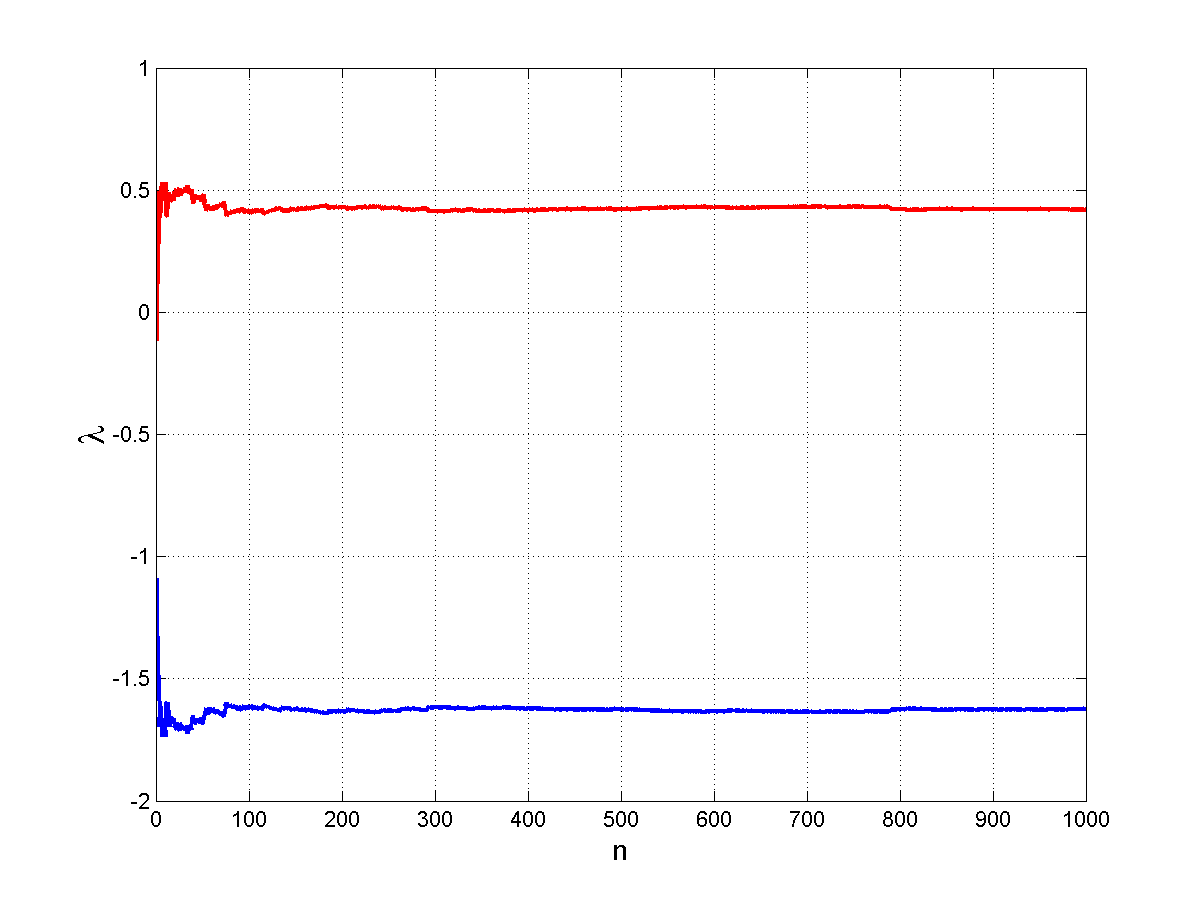
\includegraphics{docs/figs/henonlyapunovgrid.png}} 
%\caption{Expoentes de Lyapunov associados ao mapa de H�non (\ref{eqhenon}) com $a=1.4$ e $b=0.3$.}
%\label{fighenonlyapunov}
%\end{figure}
%
%O artigo cl�ssico de \citeonline{lor/63} foi um dos primeiros trabalhos a descrever movimentos ca�ticos a partir de um sistema de EDO's, como uma aproxima��o para a din�mica de uma camada de fluido convectiva. Suponha que esta camada seja mais quente na base do que no topo (conforme a Figura~\ref{figconveclorenz}), e que a diferen�a de temperatura $\Delta t$ seja suficiente grande. Sob estas condi��es o ar mais quente se eleva, deslocando o ar mais frio que est� por cima, provocando um movimento convectivo permanente. Se a diferen�a de temperatura aumentar ainda mais, o escoamento convectivo permanente � perturbado e se instala um movimento turbulento mais complicado~\cite{boyce/99}.
%
%\begin{figure}[ht]
%\centering \resizebox{13cm}{!}{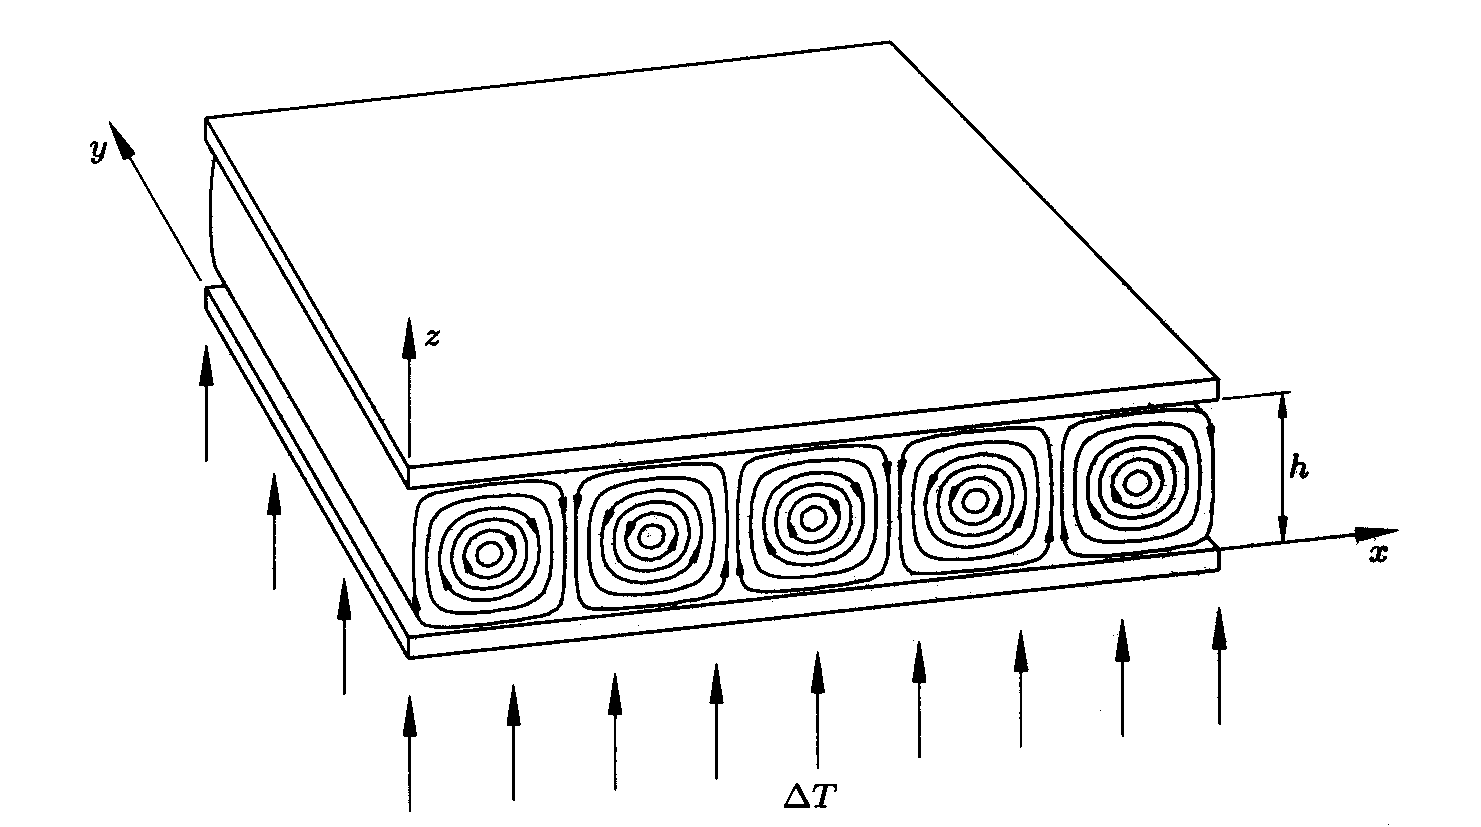
\includegraphics{docs/figs/rolo.png}} 
%\caption{Movimento convectivo de uma camada de fluido, com diferen�a de temperatura $\Delta t$ entre a placa inferior e a superior que o delimita.}
%\FONTE{Adaptada de \citeonline{argyris/94}.}
%\label{figconveclorenz}
%\end{figure}
%
%Ao investigar este fen�meno, Lorenz foi levado, por um processo complexo cuja descri��o n�o � o enfoque deste trabalho, ao sistema aut�nomo n�o-linear de EDO's
%\begin{equation}
%\begin{array}{ccc} dx/dt & = & \sigma(-x+y) \\ dy/dt & = & rx-y-xz \\ dz/dt & = & -bz+xy \end{array}
%\label{eqsistemalorenz}
%\end{equation}
%
%As Equa��es~(\ref{eqsistemalorenz}) s�o comumente denominadas equa��es de Lorenz. Pode-se observar que a segunda e a terceira equa��es envolvem n�o-linearidades quadr�ticas. A vari�vel $x$, est� relacionada � intensidade do movimento do fluido, enquanto as vari�veis $y$ e $z$ est�o relacionadas a varia��es de temperatura nas dire��es horizontal e vertical. As equa��es de Lorenz tamb�m envolvem tr�s par�metros $\sigma$, $r$ e $b$, todos reais e positivos. Os par�metros $\sigma$ e $b$ dependem do material e das propriedades geom�tricas da camada fluida. No caso da atmosfera, valores razo�veis destes par�metros s�o 
%$\sigma=10$ e $b=8/3$~\cite{lor/63}. O par�metro $r$, por outro lado, � proporcional � diferen�a de temperatura $\Delta t$, e em todas as simula��es posteriores assumir� valor $28$. Desta forma, o Sistema~(\ref{eqsistemalorenz}) assume uma forma particular, dada por
%\begin{equation}
%\begin{array}{ccc} dx/dt & = & 10(-x+y) \\ dy/dt & = & 28x-y-xz \\ dz/dt & = & -8/3z+xy \end{array}
%\label{eqsistemalorenzpart}
%\end{equation}
%
%A Figura~\ref{figlorenzx}(a) apresenta um gr�fico de valores calculados de $x$ em fun��o de $t$, ou seja, a evolu��o no tempo da vari�vel de estado $x$, que � parte da solu��o do Sistema~(\ref{eqsistemalorenzpart}). Note que a solu��o oscila entre valores positivos e negativos de uma maneira aparentemente err�tica. Na realidade, o gr�fico de $x$ contra $t$ assemelha-se ao de uma oscila��o aleat�ria, embora as equa��es de Lorenz sejam inteiramente determin�sticas e a solu��o seja completamente determinada pelas condi��es iniciais. N�o obstante, a solu��o aparenta, tamb�m, uma certa \textit{regularidade}, pois a freq��ncia e a amplitude das oscila��es s�o essencialmente constantes no tempo.
%
%As solu��es das equa��es de Lorenz s�o tamb�m muito sens�veis a perturba��es nas condi��es iniciais. A Figura~\ref{figlorenzx}(b) mostra os gr�ficos dos valores calculados de $x$ contra $t$ para duas solu��es com condi��es iniciais bastante pr�ximas. As duas solu��es ficam bastante pr�ximas uma da outra, at� $t$ nas vizinhan�as de $10$, e depois se tornam bastante diferentes, parecendo n�o ter qualquer rela��o m�tua. Esta propriedade atraiu particularmente a aten��o de Lorenz no seu trabalho original sobre as equa��es, e que tal fato deve estar relacionado � impossibilidade de se ter previs�es a longo prazo das condi��es meteorol�gicas~\cite{boyce/99}.
%
%\begin{figure}[ht]
%\centering 
%\resizebox{15cm}{!}{\includegraphics{docs/figs/lorenzst.png}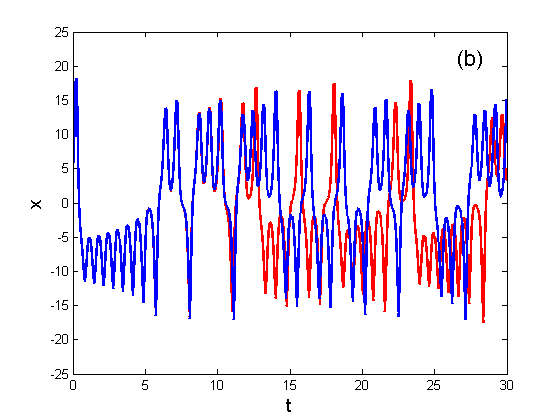
\includegraphics{docs/figs/lorenzstci.png}}
%\caption{S�ries temporais obtidas a partir da integra��o do Sistema~(\ref{eqsistemalorenzpart}). (a) condi��o inicial de $(5,5,5)$. (b) condi��o inicial da curva em azul � de $(5,5,5)$ enquanto que a da curva em vermelho � de $(5.01,5,5)$.}
%\label{figlorenzx}
%\end{figure}
%
%A Figura~\ref{figlorenzatratorproj} apresenta uma trajet�ria que principia em $(5,5,5)$ no espa�o de fase tridimensional, que se desenvolve em um atrator ca�tico cuja dimens�o de capacidade � de aproximadamente $2.16$~\cite{argyris/94}, como tamb�m suas proje��es nos planos $xy$, $xz$ e $yz$. Pode-se observar que a trajet�ria sobre o atrator nunca repete o mesmo caminho; contudo, ela est� confinada (atra�da) em uma regi�o limitada do espa�o de fase. Tal trajet�ria se alterna sobre um dos dois l�bulos, onde cada um deles cont�m um ponto cr�tico inst�vel, e este processo � repetido indefinidamente.
%
%\begin{figure}[ht]
%\centering \resizebox{13cm}{!}{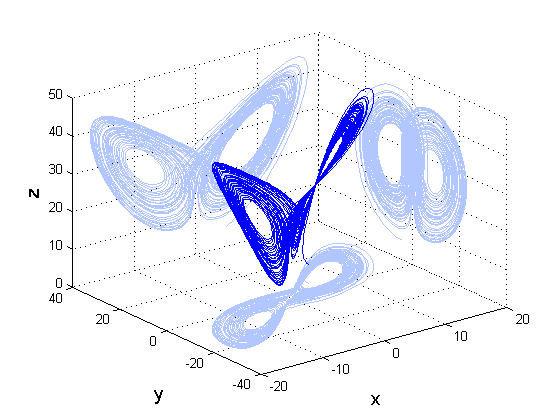
\includegraphics{docs/figs/lorenzatratorproj.png} } 
%\caption{O atrator ca�tico de Lorenz com condi��o inicial $(5,5,5)$, e suas proje��es nos planos $xy$ e $xz$ e $yz$.}
%\label{figlorenzatratorproj}
%\end{figure}
%
%Segundo \citeonline{wolf/85} os expoentes de Lyapunov associados ao Sistema~(\ref{eqsistemalorenz}) (com $\sigma=16$ e $b=4.0$ e $r=45.92$) s�o dados por
%$\lambda_{1}=2.16$, $\lambda_{2}=0$ e $\lambda_{3}=-32.4$. Desta forma, a din�mica ca�tica presente nesse sistema parece se confirmar pela presen�a de um expoente de Lyapunov positivo~\cite{wolf/85}.
%
%Quando as equa��es que governam um sistema din�mico s�o conhecidas, o estudo das caracter�sticas de suas solu��es e de seus invariantes podem revelar comportamentos complexos e interessantes. Por�m, em situa��es reais raramente se disp�e de um conjunto de equa��es diferenciais ou mesmo um mapa que descreva o comportamento do sistema. Em geral, monitora-se uma �nica vari�vel, a partir de um experimento que se sabe de antem�o depender de outras vari�veis. Desta forma, obt�m-se uma s�rie temporal de medidas semelhantes �s exibidas pelas docs/figs~(\ref{figlorenzx}) ou (\ref{figuralogis}) (admitindo-se o n�o-conhecimento de suas equa��es) e n�o se tem acesso �s outras vari�veis relevantes. A an�lise de s�ries temporais com base na teoria de sistemas din�micos � um dos temas centrais do Cap�tulo~\ref{caputiltecnicas}.
%
% 
%\section{Turbul�ncia}
%\label{secturb}
%
%\subsection{Introdu��o}
%
%O primeiro esbo�o de um fluxo turbulento, com diversos graus de realismo, foi feito por Leonardo da Vinci no s�culo XV (conforme Figura~\ref{figleonardo}). Para ele o movimento da �gua em ``redemoinhos'' era devido em parte � sua corrente principal, como tamb�m por movimentos contr�rios e aleat�rios. Da Vinci nomeou tal fen�meno de ``la turbolenza''~\cite{richter/70}. 
%
%\begin{figure}[ht]
%\centering \resizebox{13cm}{!}{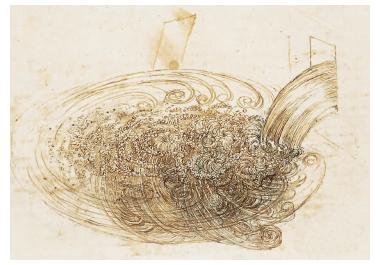
\includegraphics{docs/figs/DaVinci3.png}}
%\centering \resizebox{10cm}{!}{\includegraphics{docs/figs/DaVincipb.png}} opcao preto e branco!!!
%\caption{Ilustra��o de Leonardo da Vinci de um fluxo em redemoinhos.}
%\FONTE{\citeonline{ecke/05}}
%\label{figleonardo}
%\end{figure}
%
%Dois aspectos das observa��es de Leonardo da Vinci t�m permanecido at� os dias de hoje. Primeiro, a separa��o do fluxo em uma parte m�dia e outra flutuante, que antecipou em quase $400$ anos a aproxima��o feita por Osborne Reynolds. Segundo, a identifica��o de ``v�rtices'' como elementos intr�nsecos no movimento turbulento. O termo ``v�rtice'', usado aqui, refere-se a v�rios tipos de estruturas turbulentas presentes no escoamento, associadas, por exemplo, ao campo de velocidade de um fluido~\cite{ecke/05}.
%
%\subsection{As equa��es de Navier Stokes}
%
%Ap�s as descri��es feitas por Leonardo da Vinci, o maior avan�o na an�lise do movimento de um fluido foi por meio de equa��es din�micas, como as equa��es de Navier Stokes (escritas durante o s�culo XIX), que descrevem a taxa de varia��o da quantidade de movimento em cada ponto de um fluido viscoso. Para um fluido com densidade constante $\rho$ e viscosidade cinem�tica constante $\nu$, as equa��es de Navier-Stokes assumem a forma 
%
%\begin{equation}
%\frac{\partial u}{\partial t}+u\cdot\bigtriangledown u=-\frac{\bigtriangledown P}{\rho}+\nu\bigtriangledown ^2u
%\label{eqns1}
%\end{equation}
%
%\begin{equation}
%\bigtriangledown\cdot u=0
%\label{eqns2}
%\end{equation}
%
%Essas equa��es modelam o escoamento de fluidos incompress�veis, laminares e turbulentos, a partir de condi��es convenientes impostas nos contornos do fluido. A Equa��o~(\ref{eqns2}) � a condi��o de continuidade (sem fontes nem sumidouros), a vari�vel $u(x,t)$ � o campo de velocidade do fluido (incompress�vel), e $P(x,t)$ � o campo de press�o determinado pela preserva��o da incompressibilidade~\cite{ecke/05}. O termo $\nu\bigtriangledown ^2u$ representa a contribui��o das for�as dissipativas lineares da Equa��o~(\ref{eqns1}), enquanto o termo $u\cdot\bigtriangledown u$ representa a contribui��o das for�as de in�rcia n�o lineares da mesma equa��o.
%
%A Figura~(\ref{figvulcao}) apresenta a erup��o explosiva do Monte St. Helens em sucessivas amplia��es, mostrando estruturas em diversos comprimentos de escala. A grande diferen�a de velocidade, resultante de for�as de cisalhamento aplicadas produzem um fluido fortemente turbulento, um estado que pode ser definido como uma solu��o das equa��es de Navier-Stokes cujas caracter�sticas exibem flutua��es espacial e temporal~\cite{ecke/05}.
% 
%A Equa��o~(\ref{eqns1}) (quando multiplicada por $\rho$ fornece for�a por unidade de volume) � simplesmente a lei de Newton para um fluido: for�a � igual massa vezes acelera��o. O lado esquerdo da mesma � a acelera��o do fluido\footnote{A acelera��o de um fluido �, por defini��o, a derivada segunda (no tempo) da trajet�ria do fluido lagrangiano $x(t)$, que descreve o movimento do fluido que estava inicialmente na posi��o $x(0)$. A primeira derivada � a velocidade lagrangiana do fluido, $dx(t)/dt$ que est� relacionada com a velocidade euleriana do fluido por $dx(t)/dt=u(t,x(t))$. Devido $u$ ser uma fun��o do tempo $t$ e da posi��o $x(t)$, que � por si mesma fun��o do tempo, a express�o euleriana para a derivada segunda lagrangiana (a acelera��o do fluido) � obtida atrav�s da regra da cadeia e igual a $du/dt=\partial u/\partial t +u\cdot\bigtriangledown u$.}, e seu lado direito � a soma das for�as por unidade de massa sobre uma unidade de volume do fluido.
%
%Acredita-se que as equa��es de Navier-Stokes cont�m toda a informa��o sobre o escoamento turbulento. Embora o problema f�sico possa em princ�pio ser completamente revelado pela solu��o dessas equa��es, dadas as condi��es iniciais e de contorno, h� uma grande dificuldade devido � sua natureza n�o-linear~\cite{welter/06}. Mesmo que fosse poss�vel obter uma solu��o completa de um escoamento turbulento, onde o campo de velocidades $u(x,t)$ pudesse ser conhecido com exatid�o em cada ponto do espa�o e a cada instante de tempo, esse tipo de conhecimento seria inaplic�vel devido � dificuldade de armazenagem e processamento da enorme quantidade de informa��o. Assim, devido os graus de liberdade envolvidos em um escoamento turbulento serem muito grandes,\footnote{Segundo \citeonline{lulandlif/59}, o n�mero de graus de liberdade em um escoamento turbulento � proporcional a $R_{e}^{9/4}$, onde $R_{e}$ � denominado n�mero de Reynolds.} uma das abordagens mais utilizadas � o tratamento estat�stico das quantidades de interesse.
%
%\begin{figure}[ht]
%\centering \resizebox{15cm}{!}{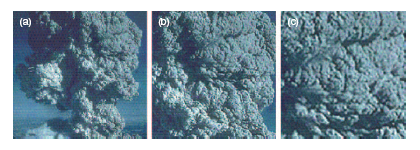
\includegraphics{docs/figs/vulcaoturb.png}}
%\caption{(a) A estrutura turbulenta de uma erup��o vulc�nica do Monte St. Helens, (b) amplia��o por um fator de $2$, (c) amplia��o por outro fator de $2$. 
%A escala caracter�stica da coluna de fuma�a � de aproximadamente $5$ Km. }
%\FONTE{\citeonline{ecke/05}}
%\label{figvulcao}
%\end{figure}
%
%
%\subsection {O N�mero de Reynolds}
%
%Como se sabe, � poss�vel distinguir entre dois tipos de escoamentos. Os escoamentos laminares, que s�o suaves e determin�sticos, e os escoamentos turbulentos, que s�o abruptos e irregulares no tempo e no espa�o. A transi��o do escoamento laminar para o escoamento turbulento � considerado um dos problemas mais complexos em mec�nica dos fluidos. As teorias de transi��o do escoamento laminar para o turbulento s�o baseadas nas pequenas perturba��es no escoamento. Estas perturba��es teriam sua origem nas colis�es intermoleculares, e dependendo da estabilidade do escoamento, seriam amplificadas ao passar do tempo e ent�o o escoamento torna-se turbulento~\cite{welter/06}.
%
%Na tentativa de criterizar a transi��o para a turbul�ncia, \citeonline{reinolds/1895} definiu uma rela��o entre for�as inerciais e viscosas que atuam nos fluidos. Esta raz�o, um par�metro adimensional, seria o ponto cr�tico de transi��o entre escoamentos laminares e turbulentos. Hoje chamado de \textit{n�mero de Reynolds} ($R_{e}$), este par�metro � proporcional � raz�o entre a contribui��o das for�as inerciais n�o lineares da Equa��o~(\ref{eqns1}) e � contribui��o das suas for�as dissipativas lineares.
%
%Se $U$ � uma velocidade caracter�stica do escoamento e $L$ � uma escala de comprimento caracter�stico, ent�o as for�as inerciais s�o da ordem de $U^{2}/L$ e as for�as viscosas s�o da ordem de $\nu U/L^{2}$. Assim, o n�mero de Reynolds do escoamento pode ser caracterizado por
%
%\begin{equation}
%R_{e}=\frac{LU}{\nu}
%\label{eqreynolds2}
%\end{equation}
%\newline
%
%Quando o numerador � muito maior que o denominador em~(\ref{eqreynolds2}), o valor de $R_{e}$ � grande e desta forma o fluxo � turbulento, caso contr�rio o fluxo � laminar (admitindo-se L constante). Em geral, considera-se que o n�mero de Reynolds cr�tico est� entre $2300$ e $3000$. Para n�meros de Reynolds menores que o n�mero de Reynolds cr�tico, a n�o-linearidade presente nas equa��es de Navier Stokes pode ser omitida, e as solu��es anal�ticas para tais equa��es correspondem a fluxos laminares. Para n�mero de Reynolds maiores que o n�mero de Reynolds cr�tico n�o h� solu��es estacion�rias est�veis e o fluido torna-se turbulento. Em particular, o fluxo se encontra na turbul�ncia completamente desenvolvida quando $R_{e}$ � muito maior que aquele obtido na transi��o para a turbul�ncia, levando-se em conta um conjunto particular de for�as e condi��es de contorno. Na natureza e em laborat�rios os escoamentos s�o em sua maioria turbulentos. Em experimentos laboratoriais em t�nel de vento $R_{e}\sim 10^{5}$ e na camada limite atmosf�rica $R_{e}\sim 10^{7}$~\cite{welter/06}. 
%
%O efeito da varia��o do n�mero de Reynolds $R_{e}$ em um fluido pode ser vista claramente na Figura~\ref{reynolds1}, que mostra graficamente o padr�o de um fluxo uniforme em um cilindro circular. O fluxo, neste caso, � visualizado por uma fuma�a ejetada da superf�cie do cilindro.
%
%Para o est�gio (a), $R_{e}\leq 1$, o fluxo � estacion�rio e n�o se separa do cilindro. Em (b), $1<R_{e}<10$, o fluxo � ainda estacion�rio mas um par de v�rtices aparecem atr�s do cilindro, que aumenta com o incremento de $R_{e}$. Em (c), $10<R_{e}<10^2$, os v�rtices est�o separados alternativamente do cilindro e alinhados em duas fileiras de v�rtices, o conhecido fen�meno dos v�rtices de K�rm�n~\cite{tomomasa/2000}. Neste caso, o fluxo n�o � mais estacion�rio e passa a ser peri�dico.
%
%Em (d), $10^2<R_{e}<10^5$, as fileiras de v�rtices tornam-se irregulares e surge um fluxo turbulento, por�m ainda laminar fora dele. Em (e), $R_{e}>10^5$, a regi�o torna-se composta de uma grande variedade de v�rtices em tamanho e dire��o, ou seja, o est�gio da turbul�ncia completamente desenvolvida. Acima de um certo valor cr�tico de $R_{e}$, no intervalo $10^5<R_{e}<10^6$, o fluxo no contorno do cilindro tamb�m torna-se turbulento.
%
%\begin{figure}[ht]
%\centering \resizebox{9cm}{!}{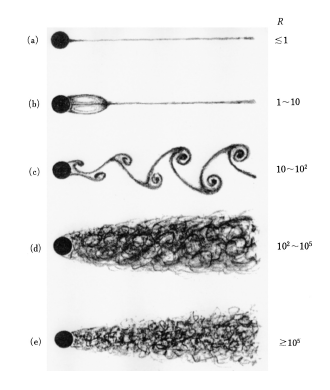
\includegraphics{docs/figs/reynoldstomomasa.png}}
%\caption{Mudan�a no padr�o do fluxo de acordo com o n�mero de Reynolds $R_{e}$.}
%\FONTE{\citeonline{tomomasa/2000}}
%\label{reynolds1}
%\end{figure}
%
% As v�rias simetrias permitidas pela equa��o de Navier-Stokes s�o sucessivamente quebradas com o incremento de $R_{e}$, ou seja, quando o fluxo deixa de ser laminar e passa a ser turbulento. Por�m, em n�mero de Reynolds ainda mais elevados h� uma tend�ncia das simetrias perdidas serem restauradas no senso estat�stico, este � o caso da turbul�ncia plenamente desenvolvida, mencionada anteriormente. 
%
%\subsection{Caracteriza��o cl�ssica da turbul�ncia}
%
%\citeonline{lumpano/64} apontam algumas propriedades de um campo turbulento, a saber
%\begin{itemize}
%\item Turbul�ncia � rotacional e dissipativa, isto �, energia mec�nica � transformada em calor;
%\item Turbul�ncia � tridimensional; 
%\item Turbul�ncia � n�o-linear. Todas as escalas est�o acopladas entre si no tempo e no espa�o;
%\item Turbul�ncia � estoc�stica. Na pr�tica n�o importa com qual cuidado as condi��es de um experimento sejam reproduzidas, o campo de velocidades n�o poder� ser predito em detalhes; 
%\item Turbul�ncia � um fen�meno cont�nuo;
%\item Turbul�ncia � difusiva. Um ponto marcado em um fluido turbulento ir� vaguear, excursionando para longe de sua posi��o inicial. Este comportamento � respons�vel pelo transporte de quantidades (massa, momentum e calor).
%\end{itemize}
%
%O car�ter estoc�stico da turbul�ncia foi questionado por \citeonline{ruelltak/71}. Tais autores introduziram uma interpreta��o alternativa dos processos turbulentos com base na teoria de sistemas din�micos, mais especificamente via ``atratores ca�ticos de baixa dimens�o''. Este assunto ser� tratado em detalhes na Se��o~(\ref{seccaosurb}).
%
%A Figura~\ref{figvelocidadevert} apresenta a evolu��o de uma vari�vel turbulenta ao longo do tempo, amostrada � $60$Hz. Pode-se observar, que mesmo � uma taxa de amostragem alta, n�o � poss�vel observar uma varia��o suave de tal vari�vel com o tempo. O mesmo comportamento � esperado com respeito ao espa�o.
%
%\begin{figure}[ht]
%\centering \resizebox{13cm}{!}{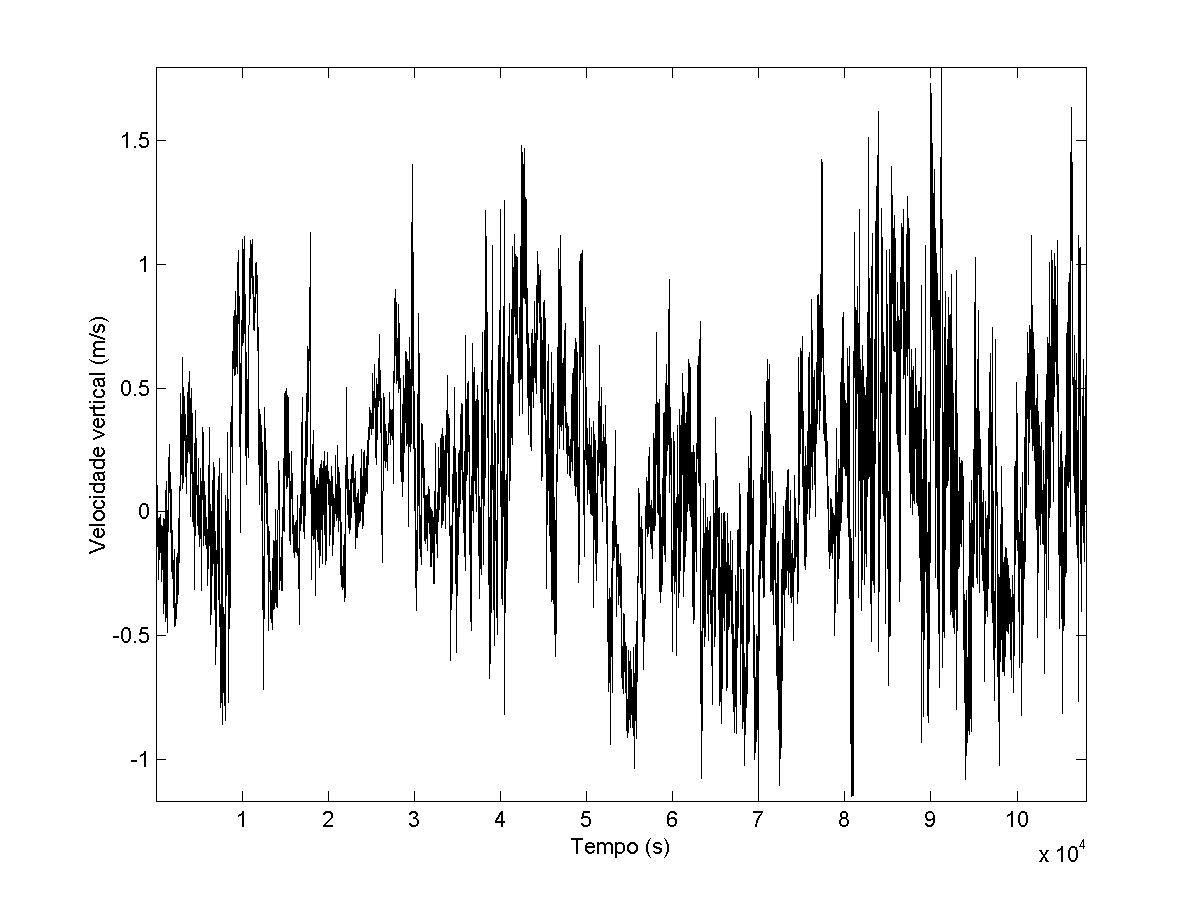
\includegraphics{docs/figs/velocidadevert.png}}
%\caption{Evolu��o temporal de uma vari�vel turbulenta amostrada � $60$Hz.}
%\label{figvelocidadevert}
%\end{figure}
%
%Pode-se imaginar, entretanto, que uma vari�vel turbulenta, como a da Figura~\ref{figvelocidadevert}, � uma composi��o de um n�mero muito grande de harm�nicos e, desta forma, pode-se pensar que a turbul�ncia � composta de uma superposi��o de v�rios harm�nicos acoplados entre si n�o linearmente. Estes harm�nicos podem ser denominados v�rtices. Seguindo esta id�ia, um campo turbulento � composto de uma superposi��o de um n�mero muito grande de v�rtices com v�rios n�meros de onda. Naturalmente, surge a necessidade de se conhecer a distribui��o da energia cin�tica entre estes n�meros de onda~\cite{welter/06}. 
%
%Segundo \citeonline{arya/88}, em escoamentos com elevado n�mero de Reynolds a \textit{Energia Cin�tica Turbulenta} (ECT) � fornecida aos v�rtices nas maiores escalas turbulentas (da ordem de $10^3$m) e, ent�o, dissipada pelos v�rtices nas menores escalas (da ordem de $10^{-3}$). A transfer�ncia dessa energia ocorre, possivelmente, por meio de um processo de cascata envolvendo todas as escalas intermedi�rias. Essa id�ia foi proposta por Richardson em $1922$~\cite{monin/71} e foi desenvolvida por Kolmogorov em sua teoria sobre turbul�ncia desenvolvida (teoria K41) e, ainda hoje, � objeto de muita discuss�o~\cite{frisch/96,nelkin/92}. V�rtices maiores colapsam-se em v�rtices menores, sucessivamente, at� atingirem as menores escalas, onde s�o destru�dos pelas for�as viscosas. Desta forma, os v�rtices menores n�o est�o diretamente ligados aos processos geradores de energia cin�tica turbulenta nas maiores escalas (flutuabilidade t�rmica e cisalhamento vertical da velocidade do vento), permitindo que as escalas intermedi�rias dessa cascata de energia tenham atributos universais a todos os escoamentos turbulentos. 
%
%A Figura~\ref{espectroesboco} � uma representa��o esquem�tica do espectro da ECT. A regi�o $1$ � a de produ��o de ECT, onde o escoamento m�dio fornece energia aos maiores v�rtices turbulentos atrav�s da flutuabilidade e do cisalhamento do vento. Kolmogorov, em $1941$, prop�s a \textit{Teoria do Equil�brio Universal} sobre a similaridade e isotropia da turbul�ncia desenvolvida na pequena escala~\cite{monin/71}. De acordo com essa teoria, para escoamentos com n�mero de Reynolds suficientemente elevados, na Regi�o $2$ da Figura~\ref{espectroesboco}, denominada de \textit{Subdom�nio Inercial} (SI), a turbul�ncia � homog�nea e isotr�pica e nela as propriedades m�dias do escoamento dependem diretamente apenas de $\epsilon$, a \textit{taxa de dissipa��o de ECT por unidade de massa}. Ainda, de acordo com a Teoria do Equil�brio Universal, a regi�o $3$ � onde a ECT transferida pela regi�o $2$ � convertida em calor pela a��o da viscosidade, fazendo com que outro par�metro al�m de $\epsilon$ seja importante nessa regi�o - a \textit{viscosidade cinem�tica} $\nu$.
%
%
%\begin{figure}[ht]
%\centering \resizebox{13cm}{!}{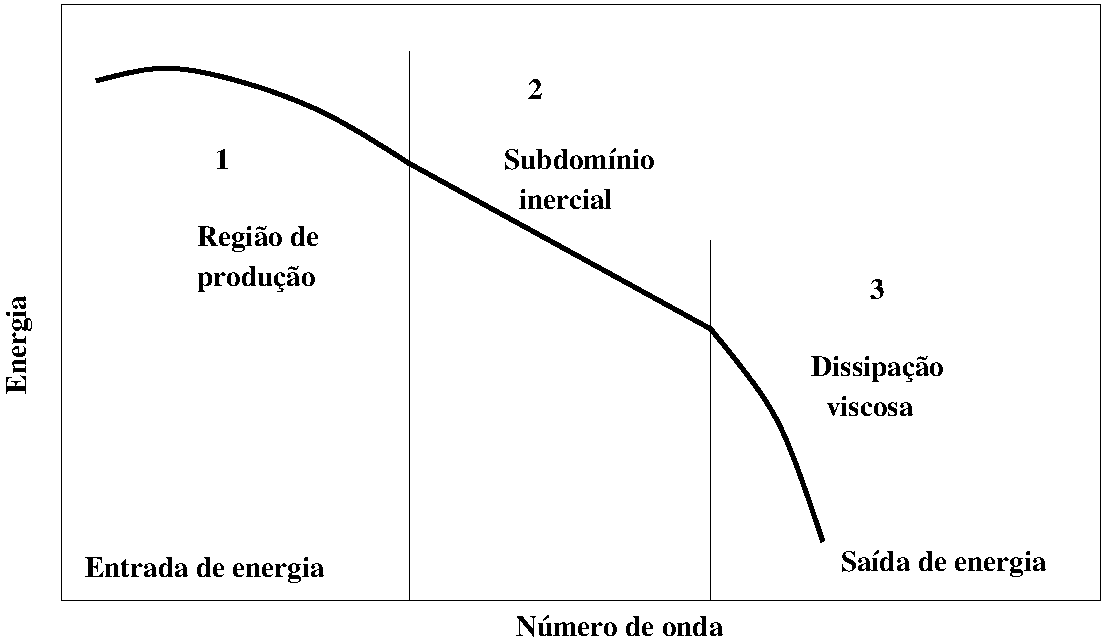
\includegraphics{docs/figs/espectroesboco4.pdf}}
%\caption{Representa��o esquem�tica do espectro da ECT em escala $\log$-$\log$.}
%\FONTE{Adaptada de \citeonline{garratt/92}}
%\label{espectroesboco}
%\end{figure}
%
% \begin{figure}[!ht]
% \begin{center}
% \resizebox{13cm}{!}{\input{docs/figs/espectroesboco5.pdftex_t}}
% \caption{Representa��o esquem�tica do espectro da ECT em escala $\log$-$\log$.}
% \FONTE{Adaptada de Garrat~\cite{garratt/92}}
% \label{espectroesboco}
% \end{center}
% \end{figure}
%
%Segundo \citeonline{frisch/96}, no SI o espectro de pot�ncia das principais grandezas turbulentas (velocidade, temperatura, umidade, etc) � caracterizado por uma lei de pot�ncia com inclina��o $-5/3$, ou seja
%
%\begin{equation}
%S_{u}(k)=a k^{-5/3}
%\label{eqespectroturb}
%\end{equation}
%onde $a$ � uma constante de propor�ao e $k$ � \textit{o n�mero de onda}. Analogamente, a lei de pot�ncia com inclina��o $-5/3$ � tamb�m obtida para $S_{u}(w)$, onde $w$ � a freq��ncia.
%
%\subsubsection{Estruturas coerentes em turbul�ncia}
%
%As estruturas coerentes t�m sido um assunto de grande relev�ncia na pesquisa em turbul�ncia~\cite{oliver/02}. Este interesse foi intensificado a partir de estudos que demonstraram que a presen�a dessas estruturas pode ser respons�vel por at� $75\%$ dos fluxos turbulentos na camada da superf�cie atmosf�rica\footnote{A por��o mais inferior da atmosfera, com extens�o de aproximadamente $1$ a $2$ Km, � denominada camada limite atmosf�rica. Esta � a regi�o mais influenciada diretamente por trocas de momento, calor e vapor de �gua na superf�cie da Terra.}~\cite{gao/89}, ou segundo outros autores por, em m�dia, $40\%$ de todo o calor turbulento e fluxos de momento \cite{lu/94,oliver/02}.
%
%N�o h� uma defini��o precisa do que sejam estruturas coerentes. Segundo \citeonline{robinson/91} estruturas coerentes de grande escala constituem uma regi�o do fluido turbulento que possui \textit{vorticidade}\footnote{O campo de vorticidade dado por $\omega (x,t)=\bigtriangledown \times u(x,t)$ � uma importante quantidade na caracteriza��o e compreens�o do fluxo turbulento. De forma geral, ele mede a rota��o de um fluxo. Na turbul�ncia 3-D, a vorticidade desempenha uma fun��o quantitativa na qual a taxa m�dia de energia dissipada $\varepsilon$ est� relacionada com o quadrado da vorticidade pela rela��o $\varepsilon=-u\langle|\omega|^2\rangle$~\cite{ecke/05}.}\textit{coerente} sobre uma significativa extens�o espacial. Essas estruturas podem ainda ser caracterizadas por uma regi�o tridimensional, onde pelo menos uma das vari�veis fundamentais do escoamento (componente de velocidade, massa espec�fica, temperatura, etc.) apresenta significativa correla��o com ela mesma ou com outra vari�vel, num intervalo de espa�o e/ou tempo suficientemente maior que as menores escalas locais do escoamento.
%
%As estruturas coerentes s�o caracter�sticas da turbul�ncia de grande escala na camada da superf�cie atmosf�rica. Sob condi��es convectivas inst�veis, elas s�o reconhecidas em s�ries temporais de flutua��es de temperatura com uma gradual eleva��o da temperatura, seguida por uma s�bita queda. Sob condi��es est�veis, este padr�o se inverte e uma gradual queda � seguida por uma s�bita eleva��o~\cite{oliver/02}. Nestas duas condi��es, a estrutura coerente � do tipo ``rampa''. 
%
%O efeito das condi��es de estabilidade sobre o comportamento em rampa das estruturas coerentes � uma conseq��ncia direta da distribui��o espacial de fontes de calor e umidade. Por exemplo, durante o dia o ar aquecido est� localizado pr�ximo � superf�cie, assim a s�bita queda de temperatura � devido � presen�a do ar mais frio que se desloca para baixo e, durante a noite, a s�bita eleva��o da temperatura est� associada com o ar mais quente que se desloca para baixo. Desde que a fonte de umidade esteja situada apenas na superf�cie, as estruturas coerentes presentes em s�ries temporais de flutua��es de umidade mostram um padr�o independente de estabilidade.
%
%\subsubsection{Intermit�ncia em turbul�ncia}
%
%A intermit�ncia � um fen�meno relacionado � presen�a de raros, por�m fortes gradientes de velocidade com acentuada localiza��o no espa�o ou no tempo. Esses gradientes s�o gerados por estruturas altamente coerentes (quase sempre n�o estacion�rias) e s�o respons�veis pelo forte aumento da taxa de dissipa��o local da ECT~\cite{camussi/97}.
%
%Segundo \citeonline{frisch/96} uma fun��o aleat�ria � intermitente se o quarto momento estat�stico normalizado, a saber, a curtose definida como
%\begin{equation}
%K(r)=\frac{\langle u_{r}^4\rangle}{{\langle u_{r}^2\rangle}^2}
%\label{eqintermitencia}
%\end{equation}
%cresce sem limites quando $r\rightarrow 0$. Desta forma, pode-se afirmar que a curtose � uma grandeza estat�stica que quantifica a presen�a de fen�menos intermitentes em um escoamento turbulento, sendo um par�metro que mede o grau de achatamento de uma \textit{Fun��o de Distribui��o de Probabilidade} (FDP). 
%
%A presen�a da intermit�ncia em um sinal turbulento confere uma forma especial � sua FDP. Para o caso da turbul�ncia atmosf�rica, as FDP's s�o, em geral, aproximadamente gaussianas nas maiores escalas do escoamento (com valores de curtose pr�ximos de $3$) e fortemente n�o gaussianas em suas menores escalas, devido ao fen�meno da intermit�ncia. As curvas da Figura~\ref{figpdfintermitente} s�o histogramas de $\Delta u_{r}=u(x+\Delta r)-u(x)$ obtidos para dist�ncias de separa��o (usando a hip�tese de Taylor $\Delta r=U\Delta t$) dadas por $\Delta r=4,40,400$ e $4000$. Para dados amostrados a $60$ Hz essas dist�ncias correspondem a $\Delta t$ de $0.06,0.66,6.66,66.66$ segundos, respectivamente. Nas menores escalas de separa��o, ocorrem grandes flutua��es com uma freq��ncia muito maior que aquela prevista para um processo gaussiano. Este fen�meno, diretamente ligado � intermit�ncia do escoamento turbulento, aparece nas FDP's sob a forma de ``asas'' ou ``caudas'' prolongadas.
%Fernando
%
%\begin{figure}[ht]
%\centering \resizebox{13cm}{!}{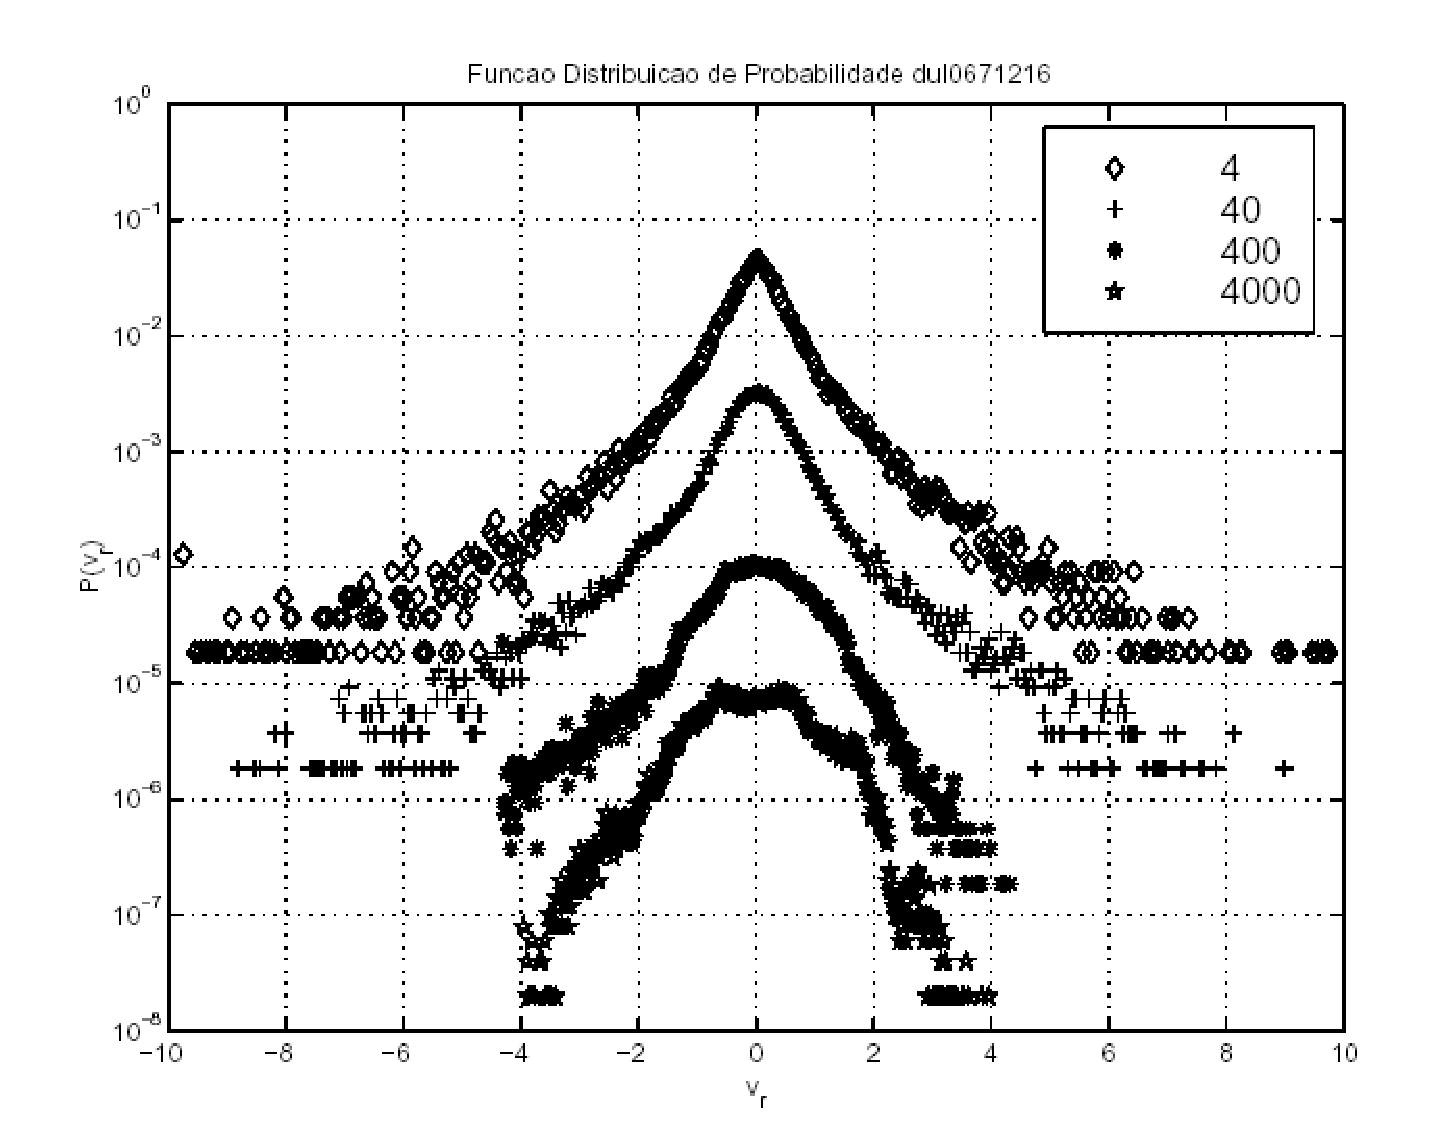
\includegraphics{docs/figs/bolzan.pdf}}
%\caption{PDF's das diferen�as de velocidade longitudinal dentro da copa da Floresta Amaz�nica, para valores de $\Delta r=4,40,400$ e $4000$.}
%\FONTE{\citeonline{bolzan/00}}
%\label{figpdfintermitente}
%\end{figure}
%
%\section{Caos e Turbul�ncia}
%\label{seccaosurb}
%
%O desenvolvimento da teoria de sistemas din�micos ca�ticos, tem fornecido importantes subs�dios � compreens�o do fen�meno da turbul�ncia. Uma conjectura feita por Landau foi a primeira tentativa para a descri��o do surgimento da turbul�ncia. Conforme sua teoria, o comportamento turbulento � causado por uma seq��ncia infinita de bifurca��es de Hopf. Desta forma, cada vez que uma bifurca��o ocorre, freq��ncias fundamentais\footnote{A cada nova freq��ncia associa-se um novo grau de liberdade ao sistema} s�o adicionadas ao sistema e a medida que cada vez mais freq��ncias ocorrem, o movimento torna-se cada vez mais turbulento~\cite{grebogi/83}. 
%
%A id�ia defendida por Landau, de que um fen�meno complexo tal como a turbul�ncia necessite de uma descri��o complexa com infinitos graus de liberdade, foi contestada a partir do estudo de Lorenz que mostrou que um sistema com apenas tr�s EDO's pode levar a comportamentos complexos e ca�ticos~\cite{argyris/94}. A concep��o de Landau foi ainda fortemente questionada for \citeonline{ruelle/91}, sobretudo pela aus�ncia tanto da sensibilidade �s varia��es nas condi��es iniciais quanto de espectros cont�nuos em sua conjectura.
%
%O trabalho pioneiro de \citeonline{ruelltak/71} introduziu uma nova e promissora perspectiva para a compreens�o do fen�meno turbulento. Esses autores foram os primeiros estudiosos a propor um poss�vel mecanismo de transi��o de um fluxo laminar para um fluxo turbulento com base na teoria de sistemas din�micos, mais especificamente por meio de atratores ca�ticos. Com base nessa abordagem Ruelle, Takens, Feigenbaum, e outros autores, investigaram ``rotas para a turbul�ncia'', ou seja, cen�rios (sucess�es de bifurca��es) nos quais um sistema com uma evolu��o temporal simples torna-se turbulento quando um ou mais de seus par�metros s�o alterados~\cite{ruellelecture/90}.  
%
%\subsection{Bifurca��o e rotas para a turbul�ncia}
%
%
%O \textit{cen�rio Ruelle-Takens}~\cite{ruelltak/71} prop�e uma rota baseada em tr�s bifurca��es consecutivas: ponto fixo $\longrightarrow$ ciclo limite $\longrightarrow$ toro\footnote{O toro $k$-dimensional $T^{k}$ pode ser entendido como o produto de $k$ c�rculos} $T^{3}$ $\longrightarrow$ atrator ca�tico (turbul�ncia). Em outras palavras, movimentos quasiperi�dicos sobre um toro $T^{3}$ (ou seja, com tr�s freq��ncias incomensur�veis) podem perder estabilidade e surgir diretamente a turbul�ncia~\cite{zeng/93,newhouse/78}. Esta rota � gen�rica e ocorre em diversos modelos matem�ticos e em experimentos de laborat�rio, por�m ela � uma rota de dif�cil compreens�o te�rica que as demais rotas mencionadas abaixo~\cite{zeng/93}.
%
%\citeonline{eckmann/81} prop�s outra rota para a turbul�ncia, que � conhecida como rota para a turbul�ncia de Feigenbaum ou de duplica��o de per�odo: uma cascata de bifurca��es de duplica��es de per�odo $p = 2^{n}(n=0,1,2,\ldots)$ que converge rapidamente para uma �rbita aperi�dica quando $n\rightarrow \infty$. Este cen�rio tem sido validado com grande �xito em diversas simula��es num�ricas e sistemas f�sicos. A duplica��o de per�odo tem sido observada em experimentos como a convec��o de Rayleigh-B�nard~\cite{zeng/93}.
%
%A quarta rota, chamada de rota para a turbul�ncia de Pomeau-Manneville, � atrav�s da intermit�ncia~\cite{pomeau/80}. No contexto de sistemas ca�ticos, o termo \textit{intermitente} refere-se a altera��es aleat�rias entre um comportamento ca�tico e regular no tempo sem envolver nenhum grau de liberdade espacial. Este conceito � diferente do significado original da \textit{intermit�ncia} na teoria hidrodin�mica da turbul�ncia, que indica ``estouros'' aleat�rios do movimento turbulento sobre a base de um fluxo laminar~\cite{zeng/93}. Nesta rota n�o h� uma clara compreens�o de quando o regime turbulento � alcan�ado nem da exata natureza desta turbul�ncia~\cite{eckmann/81}. 
%
% Especificamente, pode-se afirmar que a rota Ruelle-Takens est� relacionada a bifurca��es do tipo Hopf, onde um par de autovalores complexos cruza o c�rculo unit�rio; a rota de Feigenbaum est� associada com bifurca��es do tipo Pitchfork, onde um autovalor cruza o c�rculo unit�rio em $-1$; e a rota Pomeau-Manneville est� associada com bifurca��es do tipo Sela-N�, onde um autovalor cruza o c�rculo unit�rio em $1$. 
%
%
%A Tabela~\ref{tabbifurca} apresenta a evolu��o da din�mica de um sistema, de um estado estacion�rio � um estado turbulento, sob a influ�ncia de diferentes sucess�es de bifurca��es.
%
%\begin{sidewaystable}
%\caption{Rotas para a turbul�ncia com base em seq��ncias de bifurca��es}
%\vspace{0.5cm}
%\begin{center}
%\resizebox{!}{3.6cm}{
%\begin{tabular}{c c c c c c c c c c c c}
%\hline 
%\multicolumn{1}{c}{\textbf{}} & \multicolumn{11}{c}{\textbf{}} \\
%\multicolumn{1}{c}{\textbf{Rotas}} & \multicolumn{11}{c}{\textbf{Seq��ncias de bifurca��es}}\\
%\multicolumn{1}{c}{\textbf{}} & \multicolumn{11}{c}{\textbf{}}\\
%\cline{1-12}
%\hline 
%\textbf{} & Ponto & $\longrightarrow$ & �rbita & $\longrightarrow$ & �rbita & $\longrightarrow$ & �rbita & $\longrightarrow$ & $\cdots$ & $\longrightarrow$ & Movimento \\
%\textbf{Landau} & estacion�rio & (Hopf) & peri�dica & (Hopf) & peri�dica & (Hopf) & peri�dica & & (Hopf) & & turbulento \\
%\textbf{} & & & �nica &  & dupla &  & tripla & & & &  \\
%& & &  &  &  &  &  & & & &  \\
%\hline
%\textbf{Ruelle-} & Ponto & $\longrightarrow$ & �rbita & $\longrightarrow$ & �rbita & $\longrightarrow$ & Atrator &  &  & & \\
%\textbf{Takens} & estacion�rio & (Hopf) & peri�dica & (Hopf) & peri�dica & (Hopf) & ca�tico &  &  & &  \\
%\textbf{} & &  & �nica &  & tripla &  &  &  &  & & \\
%& & &  &  &  &  &  & & & &  \\
%\hline
%\textbf{} & Ponto & $\longrightarrow$ & �rbita & $\longrightarrow$ & �rbita & $\longrightarrow$ & �rbita & $\longrightarrow$ & $\cdots$ & $\longrightarrow$ & Atrator \\
%\textbf{Feigenbaum} & estacion�rio & (Hopf) & peri�dica & (Duplica��o & peri�dica & (Duplica��o & peri�dica &  & (Duplica��o &  & Ca�tico \\
%\textbf{} & & & �nica & de & �nica & de & �nica &  & de &  &  \\
%\textbf{} & & & (per�odo $T$) & per�odo) & (per�odo $2T$) & per�odo) & (per�odo $4T$) &  & per�odo) &  &  \\
%& & &  &  &  &  &  & & & &  \\
%\hline
%\textbf{Pomeau-} & Ponto & $\longrightarrow$ & �rbita & $\longrightarrow$ & Movimento &  &  &  &  &  & \\
%\textbf{Manneville} & estacion�rio &(Hopf) & peri�dica &  & ca�tico &  &  &  &  &  &  \\
%\textbf{} & & & �nica &  & intermitente &  &  &  &  &  &  \\
%\hline
%\end{tabular}}
%\begin{flushleft}
%\tamfonte: {Adaptada de \cite{miles/84}}
%\end{flushleft}
%\label{tabbifurca}
%\end{center}
%\begin{flushleft}
%\vspace{0.2cm}\hspace{1.6cm}\tamfonte: {Adaptada de \citeonline{miles/84}}
%\end{flushleft}
%\end{sidewaystable}
%
%
%De modo geral, todas as rotas descritas acima, est�o relacionadas � turbul�ncia em seu est�gio inicial (turbul�ncia fraca), ou seja, quando a mesma pode ainda ser descrita por um n�mero reduzido de graus de liberdade~\cite{chenmin/05}. Segundo \citeonline{zeng/93}, a compreens�o do fen�meno turbulento ser� alcan�ada quando o mecanismo inicial que lhe deu origem for completamente entendido. Tal id�ia justifica, em grande parte, a import�ncia do estudo das rotas para a turbul�ncia. Sob essa perspectiva, a turbul�ncia fraca e caos possuem caracter�sticas em comum, j� que ambos apresentam comportamentos irregulares em sua evolu��o temporal e podem ainda ser descritos por um conjunto reduzido de equa��es diferenciais determin�sticas. Em contrapartida, a turbul�ncia totalmente desenvolvida (com elevados n�meros de Reynolds) envolve irregularidades de car�ter temporal e espacial e s� pode ser descrita por um n�mero de graus de liberdade elevado.
%
%\subsection{Caracteriza��o da turbul�ncia via atratores ca�ticos}
%
%Desde que Lorenz introduziu seu modelo inspirado em din�mica dos fluidos (conforme Se��o~\ref{seccaos} deste cap�tulo), conjectura-se que a atmosfera possui um intr�nseco limite de previsibilidade e que a din�mica atmosf�rica � governada por um atrator ca�tico~\cite{weber/95}. 
%
%Diversos trabalhos confirmam a exist�ncia de atratores na atmosfera, com base em s�ries temporais turbulentas. Esses atratores foram detectados, de maneira geral, a partir da t�cnica da reconstru��o de espa�o de fase~\cite{tak/81}, que ser� discutida em detalhes no Cap�tulo~\ref{caputiltecnicas}. \citeonline{xin/01} detectaram a exist�ncia de atratores ca�ticos, com dimens�o de correla��o entre $3$ e $7$, a partir de dados turbulentos observados na camada limite atmosf�rica. Esses dados foram amostrados a $16$ Hz e incluem medidas de temperatura, umidade e velocidade do vento em tr�s dire��es, obtidos na prov�ncia de Gansu e em Beijing, China. 
%
% Diversos trabalhos confirmam a exist�ncia de atratores de baixa dimens�o na atmosfera, com base em s�ries temporais turbulentas. Esses atratores foram detectados a partir da t�cnicas como a reconstru��o de espa�o de fase \ref{eqtakensreconst}, pelo algoritmo de Grassberger e Procaccia \ref{eqcorr1} e ainda pelo algoritmo de Wolf~\cite{wolf/85}. Xin \textit{et al} \cite{xin/01} detectaram a exist�ncia de atratores estranhos, com dimens�o entre $3$ e $7$, a partir de dados turbulentos observados na camada limite atmosf�rica. Esses dados foram amostrados a $16$ Hz e incluem medidas de temperatura, umidade e velocidade do vento em tr�s dire��es, obtidos na prov�ncia de Gansu e em Beijing, China. 
%
%\citeonline{jaramillo/93} analisaram $24$ s�ries temporais de velocidade do vento e flutua��es de temperatura, amostrados a $10$ Hz, em per�odos de $30$ minutos, sobre condi��es atmosf�ricas inst�veis, e concluiram que atratores ca�ticos com baixa dimens�o, com dimens�o de correla��o entre $4$ e $6$, governam a din�mica da baixa atmosfera de Ont�rio, Canad�. 
%
%A partir de dados de tr�s componentes do vento, medidos em Almaraz (C�ceres, Espanha) � $18$ Hz, \citeonline{gallego/01} identificaram atratores ca�ticos para a turbul�ncia convectiva com dimens�o de correla��o de aproximadamente $6$ e para a turbul�ncia mec�nica com dimens�es de correla��o variando entre $7$ e $9$. 
%
%Alguns trabalhos negam a exist�ncia de atratores ca�ticos na atmosfera. Nenhum ind�cio de um atrator foi encontrado nas an�lises realizadas por \citeonline{weber/95} com base em s�ries temporais turbulentas das componentes vertical e horizontal da velocidade do vento, amostradas � $21$ Hz. \citeonline{loratrat/91} afirma que n�o h� raz�o alguma para acreditar que um sistema din�mico complexo, como o clima, possua um atrator de baixa dimens�o associado. Segundo Lorenz, o valor da dimens�o de correla��o obtido em diversas an�lises, com base em s�ries temporais clim�ticas, pode estar relacionado � dimens�o de um conjunto de subsistemas de baixa dimens�o ``fracamente'' acoplados~\cite{loratrat/91}, e n�o � dimens�o de um atrator associado ao sistema como um todo. A validade ou n�o deste cen�rio ser� investigada no Cap�tulo~\ref{caputiltecnicas}. Essa quest�o acerca da dimens�o de um eventual atrator ca�tico associado � din�mica da atmosfera est� ainda em aberto, aguardando novos experimentos e o desenvolvimento de m�todos inovadores de an�lise de s�ries temporais.
 % 2o capítulo
    %%%%%%%%%%%%%%%%%%%%%%%%%%%%%%%%%%%%%%%%%%%%%%%%%%%%%%%%%%%%%%%%%%%%%%%%%%%%%%%%
% CAP�TULO 4

\chapter{ASPECTOS GERAIS DAS T�CNICAS UTILIZADAS}
\label{caputiltecnicas}

Neste cap�tulo � feita uma descri��o detalhada dos m�todos e dos algoritmos dispon�veis para a caracteriza��o de caos determin�stico presente em s�ries temporais experimentais. Tal descri��o ser� focada nos procedimentos mais utilizados para a reconstru��o da din�mica, para o c�lculo de dimens�o de atratores e do espectro de expoentes de Lyapunov. S�o abordados alguns problemas e limita��es, do ponto de vista num�rico, associados aos algoritmos utilizados, como tamb�m as dificuldades encontradas no tratamento de sinais experimentais. 

\section{Caos em s�ries temporais}

\subsection{Introdu��o}

\citeonline{alligood/97} afirmam que ``Obviamente, a id�ia de que um experimento real possa ser governado por um conjunto de equa��es � uma fic��o. Um conjunto de equa��es diferenciais, ou um mapa, pode modelar um sistema apenas de forma o suficiente para fornecer resultados �teis''. Por outro lado, a informa��o completa de todos os graus de liberdade de um sistema din�mico complexo na natureza � raramente conhecida em sua totalidade. Por exemplo, em um fluido, esta informa��o deveria incluir sua velocidade em todas as posi��es como fun��o do tempo, o que � invi�vel na pr�tica. Neste contexto, torna-se importante analisar sistemas din�micos sem que se conhe�a detalhes sobre a sua din�mica interna, ou seja, sistemas que n�o possuem um modelo matem�tico estabelecido. Uma alternativa para isso � a an�lise de s�ries temporais que podem ser obtidas diretamente a partir de um experimento~\cite{kantz/97}.

De uma maneira geral, em um experimento monitora-se uma �nica vari�vel do sistema, que se sabe de antem�o depender das outras. Ou seja, obt�m-se uma s�rie temporal de medidas e, na maioria dos casos, n�o se tem acesso �s outras vari�veis relevantes (muitas vezes n�o se sabe ao certo sequer quantas s�o) e muito menos se disp�e de um modelo (equa��es diferenciais ou mapas) que descreva o comportamento do sistema. Caso se soubesse exatamente quais s�o as vari�veis relevantes e as mesmas pudessem ser medidas simultaneamente, poderia ser constru�do um espa�o de fase do sistema e nele representar a din�mica do sistema~\cite{aguirre/00}.

Nesta se��o apresenta-se, de maneira geral, um resumo de diversas t�cnicas utilizadas na identifica��o de s�ries temporais ca�ticas, discutem-se suas principais limita��es e enumeram-se quais informa��es pode-se extrair de sinais experimentais atrav�s desses procedimentos. Sempre que poss�vel, tais t�cnicas ser�o validadas a partir de uma s�rie temporal que apresenta comportamento ca�tico, a saber, a componente $x$ do sistema de Lorenz, que foi obtida a partir da solu��o num�rica do Sistema~(\ref{eqsistemalorenzpart}) pelo m�todo de Runge-Kutta de quarta ordem.

\subsection{A An�lise Tradicional de Sinais Experimentais}
\label{secanalisetrad}

A identifica��o de processos regulares pode ser feita atrav�s do uso de m�todos cl�ssicos. Incluem-se entre eles: a \textit{an�lise espectral} (espectro de pot�ncias) e a \textit{fun��o de autocorrela��o}, os quais ser�o introduzidos a seguir.

Seja a evolu��o de um sistema din�mico dada por uma fun��o $f(t)$, ou, quando resultado de uma s�rie de medidas realizadas a intervalos de tempos regulares $\Delta t$, representada por uma s�rie temporal da forma

\begin{equation}
{x_{n}}=x(t_{n}), \;\;\;\; t_{n}=n\Delta t
\label{eqserietemp}
\end{equation}

Sob condi��es bem gerais, uma fun��o $f(t)$ pode ser considerada como sendo a superposi��o de um n�mero (eventualmente infinito) de componentes peri�dicas. A determina��o do peso relativo de cada uma dessas componentes � chamada de \textit{an�lise espectral}. Se $f(t)$ � peri�dica, seu espectro pode ser representado como a combina��o linear de oscila��es cujas freq��ncias s�o m�ltiplos inteiros da freq��ncia b�sica $\omega$. Essa combina��o linear � chamada \textit{s�rie de Fourier}~\cite{papoulis/62}. Quando $f(t)$ � n�o-peri�dica, o espectro de freq��ncias varia continuamente e usa-se a chamada \textit{transformada de Fourier} para representar $f(t)$ em termos dessas freq��ncias~\cite{papoulis/62}. Escreve-se a transformada de Fourier de $f(t)$ como
\begin{equation}
f(\omega)=\int_{-\infty}^{+\infty}e^{-i\omega t}f(t)dt
\label{eqfouriercont}
\end{equation} 

O espectro de pot�ncias $P(\omega)$, que indica o ``peso relativo'' com que a freq��ncia $\omega$ comparece na composi��o de $f(t)$, � definido como o quadrado do m�dulo de $f(\omega)$, ou seja,
\begin{equation}
P(\omega)=\left|f(\omega)\right|^2
\label{eqespectrocont}
\end{equation} 

Na situa��o de interesse pr�tico, disp�e-se de uma s�rie temporal finita e discreta da forma~(\ref{eqserietemp}). Se $N$ � o n�mero total de pontos na s�rie, ent�o ${x_{n}}$ corresponde a um tempo total de medida $t_\textrm{max}=N\Delta t$. A transformada discreta de Fourier, de uma s�rie temporal, � definida por uma outra s�rie $\widehat{x}_{k}$ tal que
\begin{equation}
\widehat{x}_{k}=\frac{1}{\sqrt{N}}\sum_{n=1}^{N}x_{n}\exp\left[i\frac{2\pi nk}{N}\right],\;\;\;\;\;\;\;k=1.\ldots,N
\label{eqfourierdis}
\end{equation} 

A s�rie temporal~(\ref{eqserietemp}) depende do tempo; por outro lado, $\widehat{x}_{k}$ depende das freq��ncias, isto �, $\widehat{x}_{k}=\widehat{x}(\omega=k\Delta f)$ com $\Delta f= 1/t_{\textrm{max}}$. O c�lculo da transformada discreta de Fourier (\ref{eqfourierdis}) pode ser feito com rapidez atrav�s do uso do algoritmo conhecido como FFT (\textit{Fast Fourier Transform})~\cite{cooleytukey/65}.

O espectro de pot�ncias $P(\omega)$ para uma s�rie temporal discreta � definido por
\begin{equation}
P(\omega)=\left|\widehat{x}_{k}\right|^2
\label{eqespectrodiscr}
\end{equation} 

S�ries temporais com evolu��es diferentes apresentam diferentes espectros de pot�ncia. Sinais peri�dicos de per�odo $T$ apresentam um pico bem definido na freq��ncia correspondente a esse per�odo. Por outro lado, s�ries temporais ca�ticas apresentam espectros de pot�ncia com uma ``banda larga'', o que indica a exist�ncia de um cont�nuo de freq��ncias. S�ries aperi�dicas sem comportamento ca�tico tamb�m podem apresentar um espectro de pot�ncia com uma banda larga, e desta forma, � necess�rio outras ferramentas para caracterizar comportamento ca�tico em s�ries temporais~\cite{tufillaro/92}. 

A Figura~\ref{lorenzespec}(b) apresenta o espectro de pot�ncias associado � vari�vel $x$, que � parte da solu��o do Sistema~(\ref{eqsistemalorenzpart}). Pode-se observar que esse espectro apresenta uma ``banda larga'', o que indica a exist�ncia de um cont�nuo de freq��ncias. Este comportamento � necess�rio, mas n�o suficiente para a caracteriza��o de uma din�mica ca�tica na s�rie temporal em estudo.

%aperi�dicas apresentam espectros de pot�ncia cont�nuos (ver Figura~\ref{lorenzespec}(b)). Portanto, um \textit{espectro de pot�ncias cont�nuo} pode definir uma s�rie temporal ca�tica, como tamb�m um processo aleat�rio. 

\begin{figure}[ht]
\centering 
\resizebox{7.2cm}{!}{\includegraphics{Figuras/lorenzst.png}} \resizebox{7.2cm}{!}{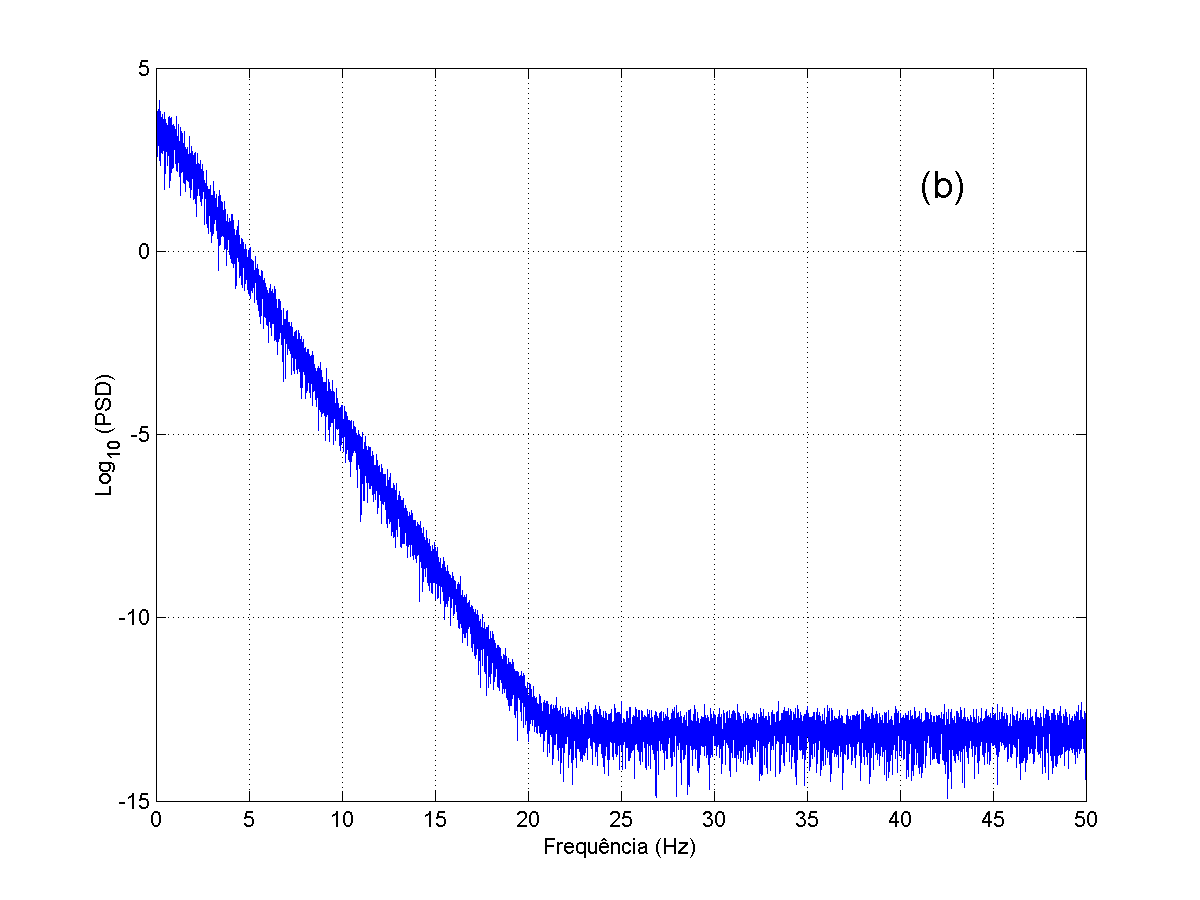
\includegraphics{Figuras/lorenzespectrogrid.png}} \\  \resizebox{7.2cm}{!}{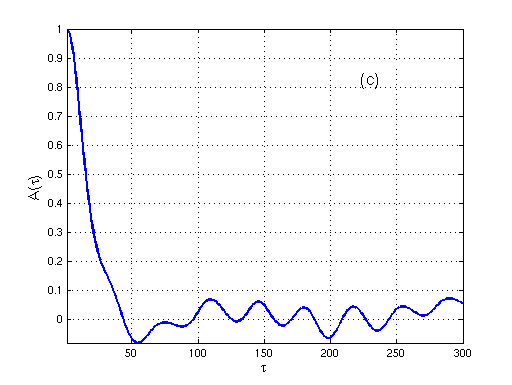
\includegraphics{Figuras/lorenzautocorrgrid.png}} 
\caption{(a) S�rie temporal ca�tica da vari�vel $x$ que � parte da solu��o do sistema~(\ref{eqsistemalorenzpart}). (b) Espectro de pot�ncia para a s�rie temporal representada em (a). (c) Fun��o de autocorrela��o para a s�rie temporal representada em (a).}
\label{lorenzespec}
\end{figure}

A fun��o de autocorrela��o $A(\tau)$ da s�rie temporal~(\ref{eqserietemp}) � definida como

\begin{equation}
A(\tau)=\frac{1}{N-\tau}\sum_{n=1}^{N-\tau}\frac{\left(x_{n}-\overline{x}\right)\left(x_{n+\tau}-\overline{x}\right)}{\sigma^2}
\label{eqautocorr}
\end{equation}
onde $N$ � o n�mero de pontos da s�rie, $\overline{x}$ sua m�dia e $\sigma^2$ sua vari�ncia. Essa fun��o representa a m�dia do produto dos valores da s�rie temporal nos instantes $t$ e $t+\tau\Delta t$ e indica por quanto tempo o valor da s�rie temporal no instante $t$ depende de seus valores pr�vios; em outras palavras $A(\tau)$ mede o grau de semelhan�a existente no sinal � medida que o tempo passa~\cite{gollub/98}. 

A fun��o de autocorrela��o~(\ref{eqautocorr}) pode ser utilizada na an�lise de uma s�rie temporal irregular. Se a s�rie temporal~(\ref{eqserietemp}) � peri�dica ou quasiperi�dica a fun��o de autocorrela��o $A(\tau)$ permanece diferente de zero quando o tempo (ou $\tau$) tende ao infinito. $A(\tau)$ de um sinal peri�dico � igualmente peri�dica, pois o sinal peri�dico volta a se parecer consigo mesmo ap�s um intervalo de tempo correspondente ao per�odo. J� para sistemas ca�ticos $A(\tau)\rightarrow 0$ quando $\tau\rightarrow \infty$~\cite{argyris/94}; a semelhan�a de uma s�rie temporal consigo mesma diminui com o tempo e acaba por desaparecer completamente (ver Figura~\ref{lorenzespec}(c)).
A fun��o de autocorrela��o de um sinal multi-peri�dico com muitas freq��ncias independentes e incomensur�veis tamb�m se confunde com aquela de um sinal ca�tico, e desta forma a caracteriza��o de comportamento, com base na fun��o de autocorrela��o, � comprometida.

A Figura~\ref{lorenzespec}(c) apresenta a fun��o de autocorrela��o associada � vari�vel $x$, que � parte da solu��o do Sistema~(\ref{eqsistemalorenzpart}). Pode-se observar que $A(\tau)\rightarrow 0$ quando $\tau\rightarrow \infty$, e desta forma, a semelhan�a da s�rie temporal consigo mesma diminui com o tempo e acaba por desaparecer completamente. Este comportamento � necess�rio, mas n�o suficiente para a caracteriza��o de uma din�mica ca�tica na s�rie temporal em estudo.

A an�lise tradicional de s�ries temporais baseada na an�lise do espectro de pot�ncias ou da fun��o de autocorrela��o n�o permite, em geral, a distin��o entre uma din�mica ca�tica determin�stica e comportamento estoc�stico. V�rios processos t�m sido desenvolvidos com essa finalidade, inclusive nos casos em que n�o se sabe (ou n�o � poss�vel) modelar ou descrever a din�mica em termos de equa��es diferenciais ou mapas. Esse assunto ser� abordado em detalhes na Se��o~\ref{subsecreconst}.

\subsection{A reconstru��o do espa�o de fase}

\label{subsecreconst}
M�todos para an�lise din�mica de s�ries temporais com comportamento ca�tico est�o ainda em desenvolvimento. Por�m, um m�todo comum � um processo dividido em duas partes~\cite{gollub/98}: 
\begin{enumerate}
\item reconstru��o do atrator ca�tico de um sistema din�mico desconhecido por meio de uma s�rie temporal;

\item determina��o de certas quantidades invariantes do sistema por meio do atrator reconstru�do. Estes invariantes podem incluir um ou mais expoentes de Lyapunov e a dimens�o do atrator. 
\end{enumerate}

Os dois processos acima citados s�o baseados na reconstru��o do espa�o de fase, que tem provado ser uma ferramenta poderosa na an�lise de sistemas f�sicos n�o-lineares com comportamento ca�tico~\cite{argyris/94}. A id�ia b�sica desta reconstru��o est� calcada no fato de que a hist�ria temporal de uma s�rie temporal cont�m informa��es sobre vari�veis de estado n�o observ�veis que podem ser usadas para determinar um estado presente. As id�ias fundamentais sobre esta t�cnica s�o creditadas a \citeonline{packard/80} e \citeonline{tak/81} e uma de suas principais caracter�sticas � a preserva��o dos invariantes do sistema (dimens�o do atrator e expoentes de Lyapunov).

A primeira tentativa de reconstruir um atrator ca�tico por meio da evolu��o de uma �nica vari�vel de estado foi realizada por \citeonline{packard/80}. Esses autores analisaram o comportamento do sistema din�mico de R�ssler\footnote{O modelo de R�ssler que satisfaz o sistema de EDO's: $dx/dt=-y-z;dy/dt=x+0.2y;dz/dt=0.4+(x-5.7)z$ possui um atrator ca�tico em seu espa�o de fase.} no espa�o de fase formado pelos eixos $x,dx/dt$ e $d^{2}x/dt^2$. Eles mostraram que, nesse novo espa�o, a figura geom�trica que caracteriza o comportamento assint�tico do sistema � topologicamente equivalente ao atrator ca�tico original. Essa figura � chamada \textit{atrator reconstru�do}. Assim, o atrator original (no espa�o $x,y,z$) e o atrator reconstru�do (no espa�o $x,dx/dt,d^{2}x/dt^{2}$) s�o caracterizados pelos mesmos valores de dimens�es e expoentes de Lyapunov. Portanto, a partir da evolu��o temporal de uma �nica vari�vel de estado, $x(t)$ neste caso, pode-se determinar as caracter�sticas do atrator associado. Segundo os autores, essa id�ia pode ser utilizada para qualquer sistema din�mico que possui um atrator ca�tico em seu espa�o de fase, como por exemplo o sistema de Lorenz (ver Figura~\ref{lorenzdiff}).

\begin{figure}[ht]
\centering 
\resizebox{15cm}{!}{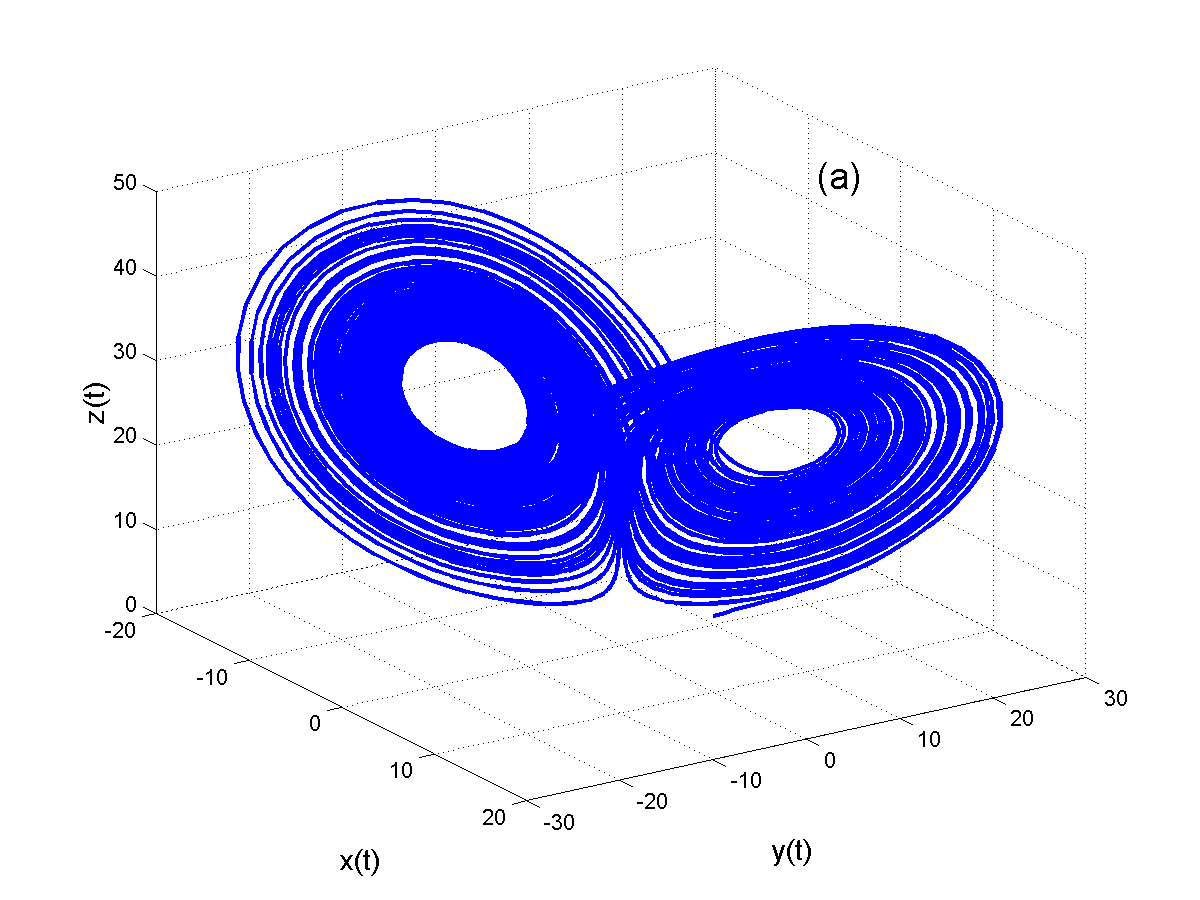
\includegraphics{Figuras/lorenzpack1.png}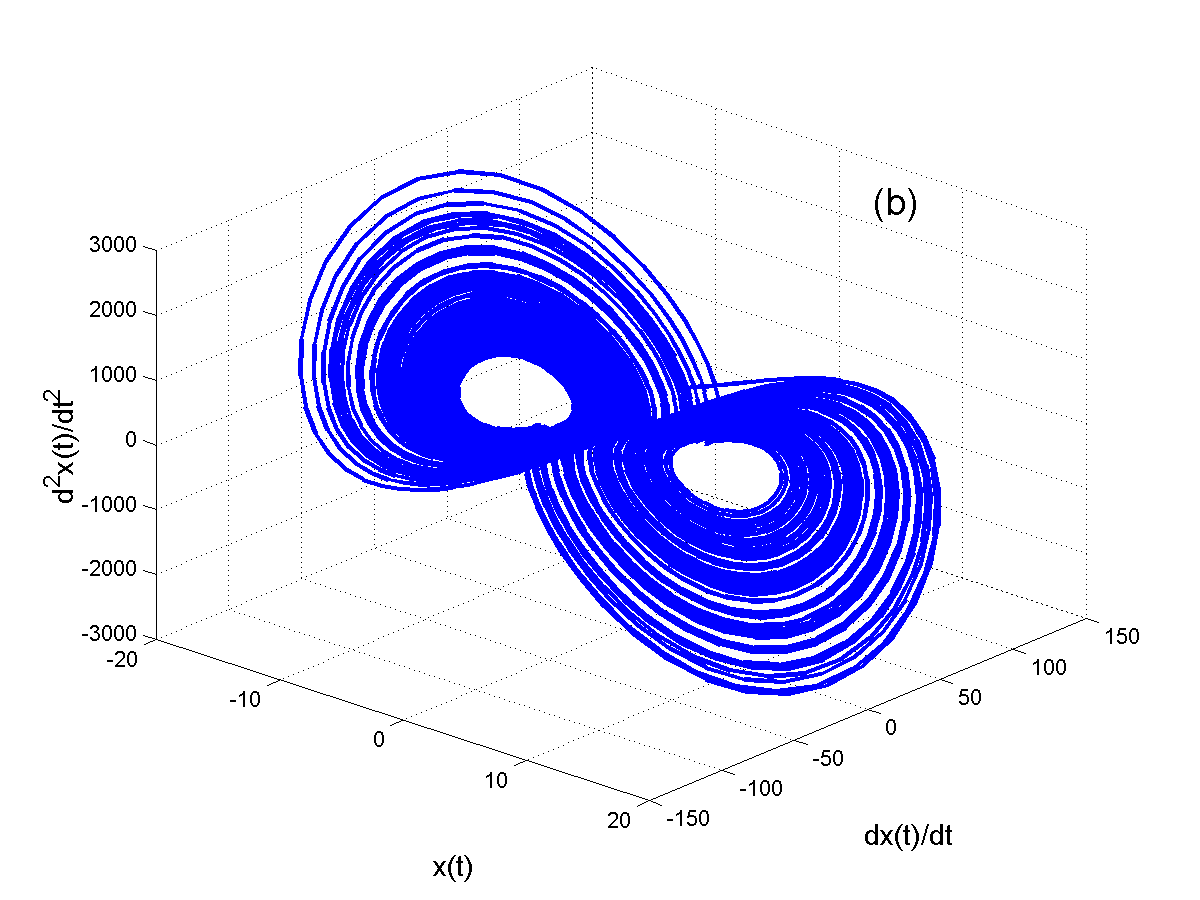
\includegraphics{Figuras/lorenzpack2.png}}
\caption{Atrator de Lorenz para o Sistema~(\ref{eqsistemalorenzpart}). (a) Atrator original. (b) Atrator reconstru�do pelo m�todo das derivadas.}
\label{lorenzdiff}
\end{figure}

As derivadas $dx/dt,d^{2}x/dt^{2}$ ou de ordens superiores podem ser aproximadas por equa��es de diferen�as com passo pequeno. Assim:

\begin{equation}
\begin{array}{rcll} \dfrac{dx}{dt} & \simeq & \dfrac{x(t+h)-x(t)}{h} & h\rightarrow 0 \\ 
                     & & &  \\
                    \dfrac{d^{2}x}{dt^{2}} & \simeq & \dfrac{x(t+2h)-2x(t+h)+x(t)}{h^2} & h\rightarrow 0 
\end{array}
\label{eqderivadapack}
\end{equation}

A determina��o num�rica de derivadas a partir de um conjunto discreto de pontos � bastante sens�vel ao ru�do, o que torna seu c�lculo muito impreciso. Al�m disso, o passo $h$ possui um valor finito, de maneira que a qualidade da aproxima��o de uma derivada por uma equa��o de diferen�a diminui com o aumento da ordem da derivada~\cite{monteiro/02}. Desta forma, tal algoritmo torna-se pouco pr�tico, principalmente se o n�mero de vari�veis de estado envolvido for grande.

Os problemas constatados com o m�todo de \citeauthoronline{packard/80} s�o evitados utilizando-se um procedimento proposto por \citeonline{tak/81}. Takens provou que, no espa�o de fase formado pelos eixos $x(t),x(t+\tau),x(t+2\tau),\ldots,x(t+(m-1)\tau)$, o atrator reconstru�do � topologicamente equivalente ao atrator ``real'', sobre o qual conhece-se apenas a evolu��o em tempo discreto da vari�vel de estado $x$. Na sua prova, Takens assumiu que a s�rie � formada por infinitos pontos e que n�o h� ru�do. Segundo Takens, se essas condi��es s�o satisfeitas, as propriedades topol�gicas do atrator reconstru�do s�o preservadas, e a reconstru��o do mesmo � feita com base na rela��o:

\begin{equation}
m\geq 2D_{0}+1,
\label{eqconditak}
\end{equation}
onde $D_{0}$ � a dimens�o de contagem de caixas do atrator associado.
 
Contudo, sua condi��o � suficiente mas n�o necess�ria, e, desta forma, a dimens�o do atrator reconstru�do pode obedecer a rela��o $m\geq D_{0}+1$ \cite{ding/93a}. Chama-se \textit{espa�o de imers�o} (``embedding space'') o espa�o no qual realiza-se a reconstru��o. Denomina-se $m$ de \textit{dimens�o de imers�o} (``embedding dimension'') e $\tau$ o \textit{passo da reconstru��o} ou \textit{tempo de atraso} (``time delay''). Note que $\tau$ deve ser um m�ltiplo do espa�amento (ou tempo de amostragem) $\Delta t$ dos pontos da s�rie temporal.

Pelo \textit{m�todo dos atrasos temporais} de Takens, a cada instante $t_{i}$, assinala-se o ponto de coordenadas $x(t_{i}),x(t_{i}+\tau),\ldots,x(t_{i}+(m-1)\tau)$ no espa�o de imers�o. Variando-se $i$ de $1$ at� $N$, obt�m-se a trajet�ria reconstru�da. Supondo que $\vec{\xi}_{\alpha}$ represente a posi��o do ponto no espa�o de imers�o no instante $t_{\alpha}$, a trajet�ria reconstru�da � formada pela seq��ncia:

\begin{equation}
\vec{\xi}_{\alpha}=(x(t_{\alpha}),x(t_{\alpha}+\tau),x(t_{\alpha}+2\tau),...,x(t_{\alpha}+(m-1)\tau))
\label{eqtakensreconst}
\end{equation} 
com $\alpha=1,\ldots,M$. As constantes $m,\tau,N,M$ relacionam-se por $N=M+(m-1)\tau$. Assumindo que a s�rie temporal � o resultado de um processo determin�stico, cada $\vec{\xi}_{\alpha+1}$ � o resultado de um mapeamento desconhecido, $\mathcal M(\vec{\xi}_{\alpha})$, ou seja,

\begin{equation}
\vec{\xi}_{\alpha+1}=\mathcal M(\vec{\xi}_{\alpha})
\label{eqtakensreconst2}
\end{equation} 

\subsubsection{A escolha do passo}

\citeonline{tak/81} demonstrou que para um n�mero infinito de pontos e na aus�ncia de ru�do a escolha do passo de reconstru��o $\tau$ � na grande maioria dos casos arbitr�ria. Entretanto, as s�ries temporais experimentais s�o finitas, usualmente contaminadas com ru�do externo e obtidas com o uso de filtros. Nessa situa��o, a reconstru��o depende da escolha correta do passo. Se o passo $\tau$ for muito pequeno $x(t),x(t+\tau)$ e $x(t+2\tau)$, por exemplo, ter�o praticamente o mesmo valor\footnote{Admite-se que a freq��ncia de amostragem, relacionada com o intervalo de tempo $\Delta t$ entre duas medidas consecutivas, � suficientemente elevada para capturar toda a estrutura fina do sinal, ou seja, que ela seja adequada para se monitorar com detalhe a evolu��o temporal do sistema.}. Como conseq��ncia, o atrator reconstru�do fica comprimido em torno da diagonal $z=y=x$, j� que $\vec{\xi}_1\simeq\vec{\xi}_2\simeq\vec{\xi}_3$, ou seja, esse atrator apresentar� uma depend�ncia linear entre $\vec{\xi}_1,\vec{\xi}_2$ e $\vec{\xi}_3$, que n�o ocorre nas componentes reais $x,y$ e $z$ (conforme Figura~\ref{figlorenzpasso}(a)). Por outro lado, como a trajet�ria real est� restrita a um volume finito do espa�o de fase, o passo $\tau$ n�o pode ser muito grande, sob pena dos vetores reconstru�dos $\vec{\xi}_i$ serem completamente n�o-correlacionados, cobrindo todo o espa�o de fase (conforme Figura~\ref{figlorenzpasso}(c)).

\begin{figure}[ht]
\centering 
\resizebox{7.2cm}{!}{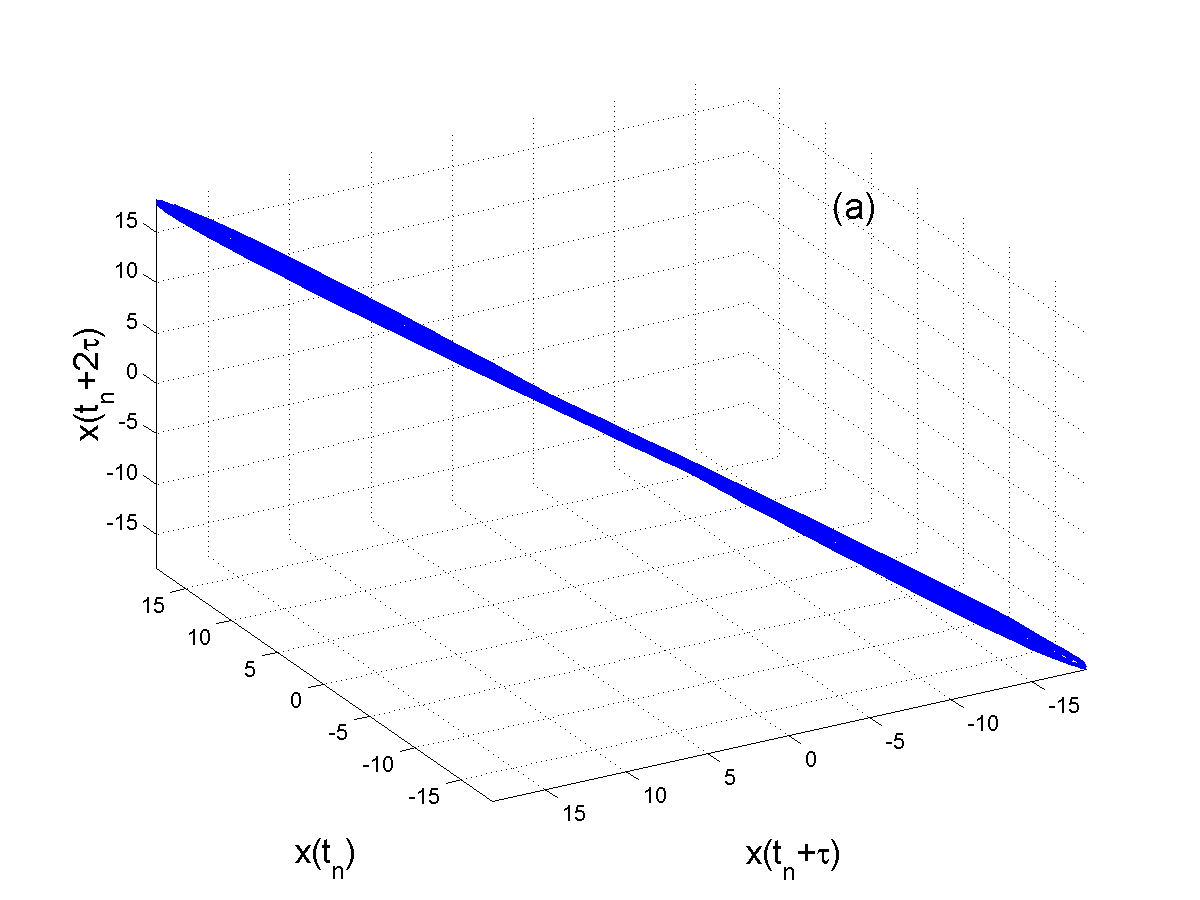
\includegraphics{Figuras/lorenzatraso1.png}} \resizebox{7.2cm}{!}{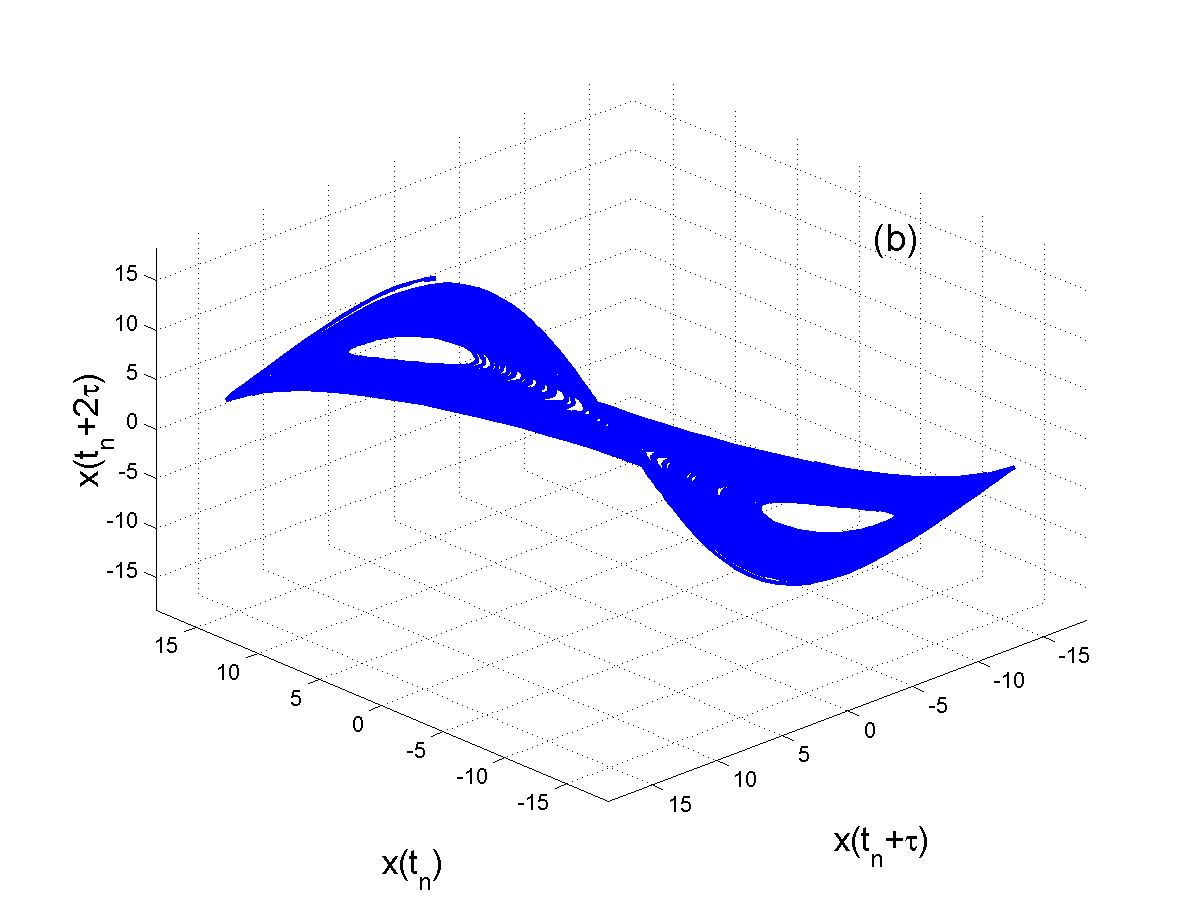
\includegraphics{Figuras/lorenzatraso2.png}} \\  \resizebox{7.2cm}{!}{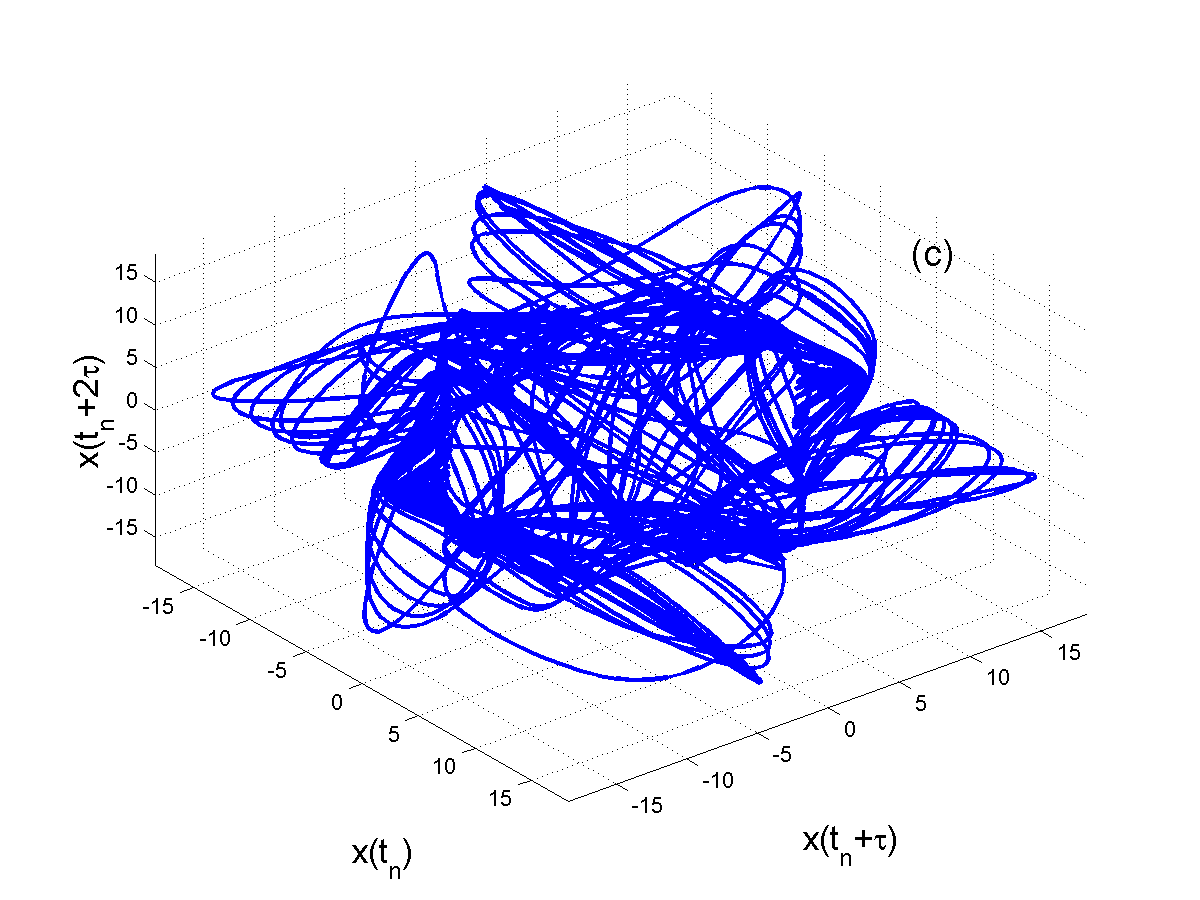
\includegraphics{Figuras/lorenzatraso3.png}} 
\caption{Exemplo da influ�ncia do passo na reconstru��o do atrator de Lorenz associado ao Sistema~(\ref{eqsistemalorenzpart}). (a) passo muito pequeno ($\tau=1$). (b) passo adequado ($\tau=12$). (c) passo muito grande ($\tau=50$).}
\label{figlorenzpasso}
\end{figure}

Diversos trabalhos t�m proposto crit�rios para orientar a escolha do passo correto~\cite{fraswi/86}. O crit�rio mais difundido, e tamb�m utilizado nesta disserta��o, consiste em examinar a correla��o entre os pares de pontos em fun��o de seu tempo de separa��o, ou seja, atrav�s da fun��o de autocorrela��o (j� definida na Se��o~\ref{secanalisetrad}). Ap�s determinar o tempo do primeiro ``zero'' desta fun��o, uma modesta fra��o deste valor � uma escolha razo�vel para o atraso $\tau$ \cite{gollub/98}.

A sensibilidade do processo de reconstru��o relativamente ao passo pode ser estimada atrav�s de um m�todo bastante pr�tico e r�pido: o chamado \textit{gr�fico de primeiro retorno}, que consiste em graficar-se $x(t_{i})\times x(t_{i}+\tau)$, reconstruindo-se para tanto vetores bidimensionais com passo $\tau$ (conforme Figura~\ref{figlorenzprimeiroret}). Uma simples inspe��o visual desse gr�fico fornece informa��es sobre os valores de $\tau$ para os quais $x(t_{i})$ e $x(t_{i}+\tau)$ est� ainda fortemente correlacionados, situa��o em que o atrator reconstru�do fica comprimido pr�ximo � diagonal e, desta forma, indica qu�o sens�vel � a reconstru��o do atrator relativamente � escolha do passo, qu�o homog�neo � o atrator e qual o n�mero t�pico de vetores reconstru�dos necess�rio para caracteriz�-lo completamente~\cite{monteiro/02}. 

\begin{figure}[ht]
\centering 
\resizebox{7.2cm}{!}{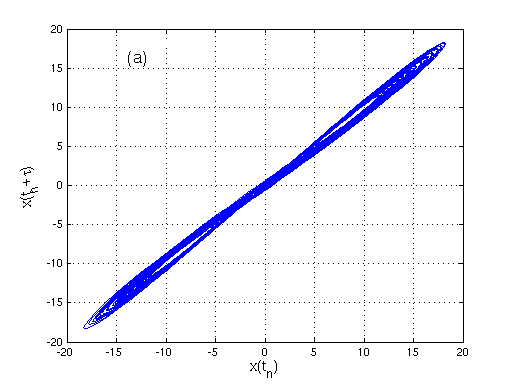
\includegraphics{Figuras/lorenzreconstbi1.png}} \resizebox{7.2cm}{!}{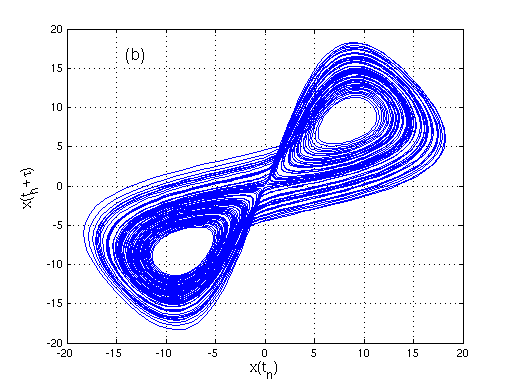
\includegraphics{Figuras/lorenzreconstbi12.png}} \\  \resizebox{7.2cm}{!}{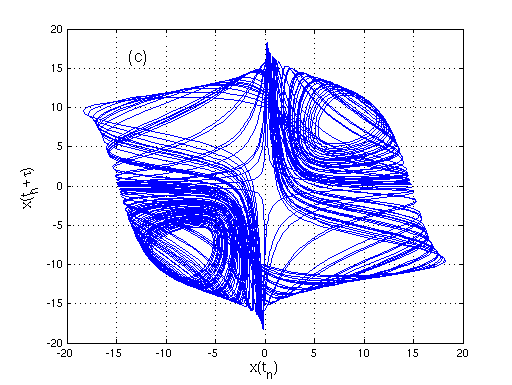
\includegraphics{Figuras/lorenzreconstbi50.png}} 
\caption{Gr�fico de primeiro retorno a partir da vari�vel $x$ que � parte da solu��o do Sistema~(\ref{eqsistemalorenzpart}). (a) $\tau=1$. (b) $\tau=12$. (c) $\tau=50$.}
\label{figlorenzprimeiroret}
\end{figure}

\subsubsection{A escolha da dimens�o de imers�o}
\label{secdimimers}

\paragraph*{Dimens�es generalizadas}
Atratores ca�ticos apresentam um comportamento irregular e os mesmos n�o preenchem completamente o espa�o de fase devido � contra��o do elemento de volume~\cite{argyris/94}. Um atrator ca�tico imerso em um espa�o de fase tridimensional � uma forma ``h�brida'' entre uma superf�cie e um objeto espacial e assim sua dimens�o est� entre $2$ e $3$, ou seja, � um fractal. Desta forma, a caracteriza��o desse atrator � realizada com base no conceito generalizado de dimens�o que no caso de atratores regulares como pontos fixos, ciclos limites e toros, coincidem com a dimens�o convencional em geometria euclidiana, ou seja, $0$, $1$ ou $2$.

Existe um conjunto infinito de dimens�es, $D_{q}$, conhecidas como dimens�es generalizadas, que definem propriedades m�tricas ou probabil�sticas de um atrator~\cite{hentschel/83}. Deixe um atrator ca�tico ser coberto por $m(\varepsilon)$ quadrados de lado $\varepsilon$, e seja $M$ o n�mero total de pontos observados no atrator. Ent�o, a probabilidade de que um ponto se encontre no $i$-�simo quadrado � obtido pela raz�o $p_{i}=M_{i}/M$, onde $M_{i}$ � o n�mero de pontos do atrator que se encontra no $i$-�simo quadrado. O conjunto infinito de dimens�es generalizadas � dado por

\begin{equation}
D_{q}=\dfrac{1}{q-1}\lim_{\varepsilon\rightarrow\infty}\dfrac{\ln \sum_{i=1}^{m(\varepsilon)}p_{i}^q}{\ln \varepsilon}
\label{eqdimgeneral}
\end{equation}

onde $q$ est� relacionado �s poss�veis defini��es da dimens�o. Quando $q=0$, a rela��o~(\ref{eqdimgeneral}) produz simplesmente a dimens�o de contagem de caixas $D_{0}$ sobre o atrator. A dimens�o de informa��o $D_{1}$ e a dimens�o de correla��o $D_{2}$ s�o obtidas no limite da Equa��o~(\ref{eqdimgeneral}) quando $q$ tende para $1$ e $2$, respectivamente. $D_{1}$ pode ser expresso como~\cite{farmer/83}

\begin{equation}
D_{1}=\lim_{\varepsilon\rightarrow 0}\dfrac{\ln \sum_{i=1}^{m(\varepsilon)}p_{i} \ln p_{i}}{\ln \varepsilon}
\label{eqdiminfor}
\end{equation}

que � conhecida como dimens�o de informa��o ou dimens�o entr�pica.

A dimens�o de correla��o, proposta por \citeonline{grassproca/83} como uma forma de caracterizar atratores ca�ticos, � dada pela rela��o

\begin{equation}
D_{2}=\lim_{r\rightarrow\ 0}\frac{\log C(r)}{\log r}
\label{eqcorr2}
\end{equation}
onde $C(r)$ � a fun��o de correla��o integral definida como

\begin{equation}
C(r)=\frac{1}{M^2}\sum_{i,j=1 \\, i\neq j}^{M} \Theta\left(r-\left \|\vec{\xi}_{i}-\vec{\xi}_{j}\right \|\right),
\label{eqcorr1}
\end{equation}
onde $M$ � o n�mero de pontos no atrator, $\|\|$ denota a norma euclidiana que quantifica a dist�ncia entre os pares de vetores em espa�os de imers�o arbitr�rios e $\Theta(x)$ � uma fun��o degrau de Heavyside, definida por
\begin{equation}
\Theta(x)=\
\left\{ \begin{array}{ccl}
 1,  &  \mathrm{se} & x\geq 0   \\
 0,  &  \mathrm{se} & x< 0
\end{array}
\right.  
\label{eqheavyside}
\end{equation}

A correla��o integral (\ref{eqcorr1}) conta a freq��ncia relativa de pares cuja separa��o � menor que a escala $r$. Note que a Equa��o~(\ref{eqcorr2}) implica que para pequenos valores de $r$, a correla��o integral $C(r)$ comporta-se como uma lei de pot�ncia $C(r)\approx r^{D_{2}}$. Conseq�entemente, o c�lculo do expoente pode ser obtido a partir de um gr�fico de $C(r)$ versus $r$ em escala $\log$-$\log$.

Para valores de $q\geq3$, \citeonline{hentschel/83} fornecem aproxima��es para as dimens�es generalizadas $D_{3},D_{4},\ldots$ associando fun��es de correla��o integral entre triplas, qu�druplas, etc. de vetores. � poss�vel mostrar que estas dimens�es est�o ordenadas da seguinte maneira: $D_{0}\geq D_{1}\ldots\geq D_{n}$, sendo que a igualdade � v�lida sob a hip�tese de que os pontos do atrator sejam uniformemente distribu�dos.

Em geral, o expoente $D_{2}$ � mais f�cil de ser estimado que o expoente $D_{0}$ devido ao grande esfor�o computacional empregado na procura da dimens�o de contagem de caixas~\cite{greenside/82}. Em diversos sistemas, a dimens�o de contagem de caixas $D_{0}$ e a dimens�o de correla��o $D_{2}$ s�o muito pr�ximas uma da outra e, desta maneira, o valor de $D_{2}$ fornece uma boa estimativa do n�mero m�nimo de equa��es diferenciais n�o-lineares necess�rias para descrever o atrator~\cite{moon/97}.

% Na pr�tica, para um conjunto finito de dados com resolu��o temporal discreta e finita exatid�o, o limite em (\ref{eqcorr2}) pode n�o ser rigorosamente alcan�ado. Por�m, em um gr�fico de $\log C(r,M)$ versus $\log r$, uma parte linear aparece para valores intermedi�rios de $r$. Sua inclina��o fornece uma estimativa da dimens�o de correla��o \cite{rudolf/95}.

% Conforme a Figura~\ref{lorenzdiff}(a) o atrator de Lorenz cuja dimens�o fractal � de aproximadamente $d=2.16$, pode ser bem representado em um espa�o de imers�o $m=3$. Contudo, em uma s�rie temporal arbitr�ria a dimens�o $d$ do atrator � desconhecida e, desta forma, o valor $m$ tamb�m o �. 

A implementa��o do algoritmo de Grassberger-Procaccia � relativamente simples. Entretanto, esse algoritmo  exige o c�lculo e a classifica��o de aproximadamente $n(n-1)$ dist�ncias, onde $n$ � o n�mero de vetores reconstru�dos pela rela��o~(\ref{eqtakensreconst}). Este procedimento consome um tempo de processamento  excessivamente longo se o algoritmo n�o � constru�do  de forma otimizada, sobretudo se a s�rie temporal for muito longa. Diversas sugest�es, simplifica��es e modifica��es t�m sido propostas~\cite{theiler/87,parker/89,malraison/83}. O procedimento adotado nesta disserta��o reduz o c�lculo de dist�ncias por considerar apenas um subconjunto de vetores reconstru�dos, escolhidos de forma aleat�ria~\cite{malraison/83}. Como a escolha � aleat�ria, espera-se que o subconjunto de dist�ncias calculadas reproduza a estat�stica do conjunto de todas as dist�ncias, mantendo inalterado o valor de $C(r)$.

Na medida em que h� limita��es experimentais fortes para a obten��o de s�ries de dados longas, esse fato, aliado ao excessivo tempo de processamento, restringe a utiliza��o do algoritmo de Grassberger-Procaccia para o caso de atratores de alta dimens�o. Na grande maioria das aplica��es a sinais experimentais, o algoritmo de Grassberger-Procaccia n�o permite estimar com seguran�a dimens�es de correla��es $D_{2}$ maiores de $4$ e $5$, as quais correspondem a dimens�es de imers�o da ordem de $9$ e $11$, respectivamente. 

A dimens�o de correla��o $D_{2}$ � uma das principais ferramentas usadas para identificar a exist�ncia de din�mica ca�tica. Caos determin�stico, em geral, � identificado se a inclina��o de $C(r)$ versus $r$ converge para um valor de satura��o, para valores cada vez mais altos da dimens�o de imers�o $m$ \cite{grassproca/83}. Em sinais determin�sticos com comportamento ca�tico, o valor $D_{2}$ alcan�a um valor m�ximo devido a natureza de baixa dimens�o do sistema. Desta forma, a dimens�o de satura��o obtida � uma aproxima��o para a dimens�o fractal do atrator. A partir da rela��o~(\ref{eqconditak}), o valor da dimens�o de imers�o $m$ pode ser estimado. O valor desta dimens�o permite ``desdobrar'' o atrator adequadamente, de modo que suas trajet�rias n�o se cruzem no espa�o de imers�o. 

A Figura~\ref{figatratorhipot} ilustra o atrator de Lorenz imerso em espa�os de fase de dimens�es $2$ e $3$, respectivamente. A imers�o no espa�o de fase de duas dimens�es d� origem a falsos cruzamentos das trajet�rias (conforme Figura~\ref{figatratorhipot} (a)). Esses falsos cruzamentos podem estar ligados a falsos vizinhos pr�ximos - um efeito que produz erros no c�lculo do expoente de Lyapunov. Somente o espa�o de fase tridimensional esbo�a este atrator completamente (conforme Figura~\ref{figatratorhipot} (b)). Este fato mostra a import�ncia da imers�o do atrator reconstru�do em um espa�o de fase adequado.

\begin{figure}[ht]
\centering 
\resizebox{15cm}{!}{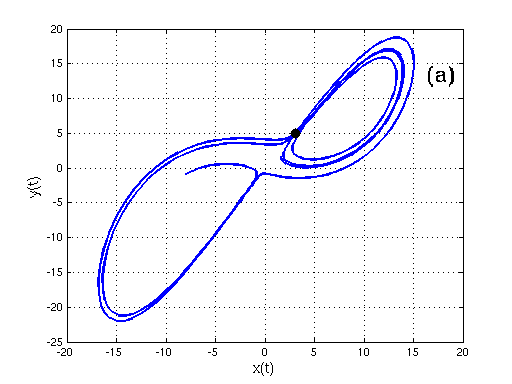
\includegraphics{Figuras/lorenzproj1.png}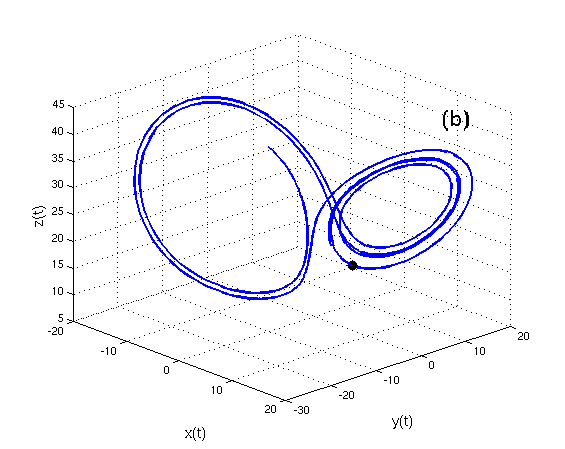
\includegraphics{Figuras/lorenzproj2.png}}
\caption{Efeito da imers�o do atrator de Lorenz em espa�os de diferentes dimensionalidades. (a) A imers�o no espa�o de fase bidimensional ocorre um falso cruzamento (marcado com um ponto em preto). (b) O atrator � completamente representado no espa�o tridimensional.} 
\label{figatratorhipot}
\end{figure}

A Figura~\ref{figlorenzdimensoes}(b) mostra a correla��o integral da s�rie temporal em $x$ de Lorenz (Figura~\ref{figlorenzdimensoes}(a)) versus a escala $r$ em diferentes dimens�es de imers�o. Pode-se observar que cada uma destas curvas possui se��es lineares, cujos valores das inclina��es, calculados via regress�o linear, saturam quando as dimens�es de imers�o s�o incrementadas. Estes valores de inclina��es em fun��o das dimens�es de imers�o que variam de $1$ a $10$ podem ser vistos atrav�s da Figura~\ref{figlorenzdimensoes}(c). Foram feitas $5$ realiza��es an�logas � descrita acima, e a dimens�o de correla��o m�dia obtida foi de $\langle D_{2}\rangle=2.105$ com desvio padr�o de $\sigma_{D_{2}}=0.01$. Ainda, na Figura~\ref{figlorenzdimensoes}(c) pode ser observada a dimens�o de correla��o obtida a partir de uma s�rie temporal aleat�ria (ru�do branco). Para este caso, o valor de $D_{2}$ n�o satura quando as dimens�es de imers�o s�o incrementadas. Este comportamento j� era esperado, pois um ru�do branco est� associado a um processo estoc�stico e n�o a uma din�mica ca�tica.

\begin{figure}[ht]
\centering 
\resizebox{7.2cm}{!}{\includegraphics{Figuras/lorenzst.png}} \resizebox{7.2cm}{!}{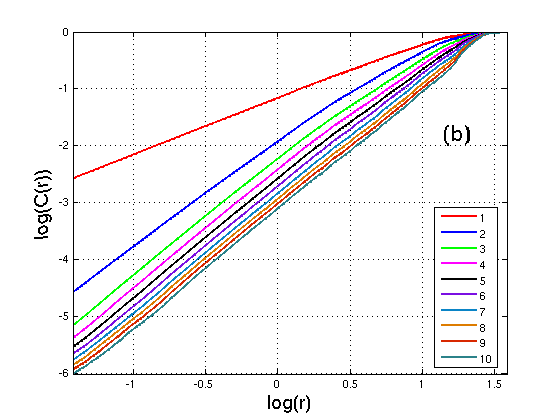
\includegraphics{Figuras/lorenzcorrelint2.png}} \\  \resizebox{7.2cm}{!}{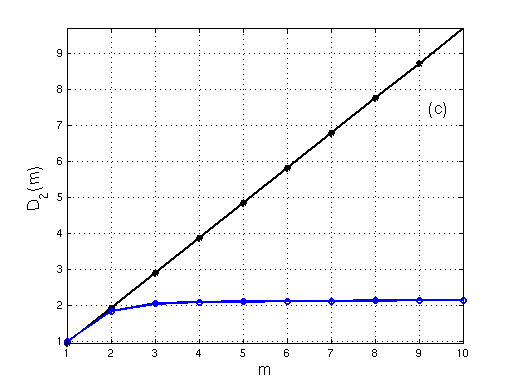
\includegraphics{Figuras/lorenzdimcorrel2.png}} 
\caption{(a) S�rie temporal obtida a partir da integra��o do Sistema~(\ref{eqsistemalorenzpart}). (b) Correla��o integral da s�rie em (a) com $m=1$ a $10$. (c) Dimens�o de correla��o de $D_{2}\langle2.105\rangle$ para a s�rie de Lorenz (curva -o- em azul) e dimens�o de correla��o infinita para uma s�rie aleat�ria (curva -*- em preto)}
\label{figlorenzdimensoes}
\end{figure}

\paragraph*{Distin��o entre din�mica de baixa dimens�o e aleatoridade}

\citeonline{osboproven/89} oferecem um contra-exemplo da vis�o tradicional de que a inclina��o de $C(r)$ versus $r$ aumenta continuamente para processos estoc�sticos, quando a dimens�o de imers�o $m$ � incrementada~\cite{grassproca/83}. Especificamente, tais autores mostraram que uma classe simples de ru�do ``colorido'', caracterizado por uma lei de pot�ncia no espectro da forma $S(w)\approx w^{-\alpha}$ conduz � satura��o em $D_{2}$ conforme a rela��o $D_{2}=2/(\alpha-1)$~\cite{osboproven/89,theilerj/91}. Este resultado tem s�rias implica��es sobre o estudo experimental de comportamento ca�tico determin�stico, j� que a observa��o de um valor finito de $D_{2}$ pode n�o ser suficiente para afirmar a presen�a de atratores ca�ticos em um sistema din�mico. 

Em contrapartida, \citeonline{provenzalesmith/92} apresentam alguns testes que podem ser usados na distin��o entre din�mica de baixa dimens�o e aleatoriedade em s�ries temporais. Esses testes s�o baseados na id�ia de se modificar algumas propriedades de uma s�rie temporal, com o intuito de verificar se a converg�ncia de $D_{2}$ depende ou n�o dessas propriedades modificadas. 

O primeiro de tais testes � denominado ``teste surrogate'' e consiste em considerar a distribui��o das fases de Fourier de uma s�rie temporal. Desta forma, � aplicada a transformada de Fourier (conforme a Equa��o~(\ref{eqfourierdis})) na s�rie em estudo. Em seguida, suas fases s�o embaralhadas uniformemente e � aplicada a transformada de Fourier inversa. A s�rie temporal obtida com este processo � aleat�ria, j� que o surrogate destr�i as correla��es existentes na s�rie temporal que lhe deu origem, por�m seu espectro de pot�ncia � similar ao da s�rie original. Se a converg�ncia de $D_{2}$ � determinada apenas pela forma do espectro (ou equivalentemente pela fun��o de autocorrela��o), ent�o os resultados n�o s�o afetados pelo embaralhamento das fases. A invari�ncia do valor de $D_{2}$ sobre as fases embaralhadas sugere fortemente que tais estimativas n�o indicam uma din�mica ca�tica~\cite{provenzalesmith/92}. 

A Figura~\ref{figlorenzsurrogate}(a) mostra a s�rie temporal obtida a partir do surrogate da s�rie temporal em $x$ de Lorenz, a Figura~\ref{figlorenzsurrogate}(b) mostra a correla��o integral obtida para dimens�es de imers�o que variam de $1$ a $10$ e finalmente a Figura~\ref{figlorenzsurrogate}(c) apresenta a dimens�o de correla��o, $D_{2}$, associada. A apar�ncia da s�rie temporal com surrogate � completamente diferente da apresentada na Figura~\ref{figlorenzdimensoes}(a) e os respectivos valores de $D_{2}$ s�o tamb�m bastante distintos (ver Figuras~\ref{figlorenzsurrogate}(c) e \ref{figlorenzdimensoes}(c)). Foram feitas $5$ realiza��es an�logas � descrita acima, e pode-se observar que a dimens�o de correla��o $D_{2}$ em todos os casos n�o satura. Esse comportamento sugere fortemente a exist�ncia de uma din�mica de baixa dimens�o na s�rie temporal de Lorenz. %Desta forma, em uma s�rie temporal arbitr�ria, a constata��o de um comportamento similar ao encontrado acima \textit{sugere} fortemente a exist�ncia de um atrator ca�tico associado~\cite{provenzalesmith/92}. 

\begin{figure}[ht]
\centering 
\resizebox{7.2cm}{!}{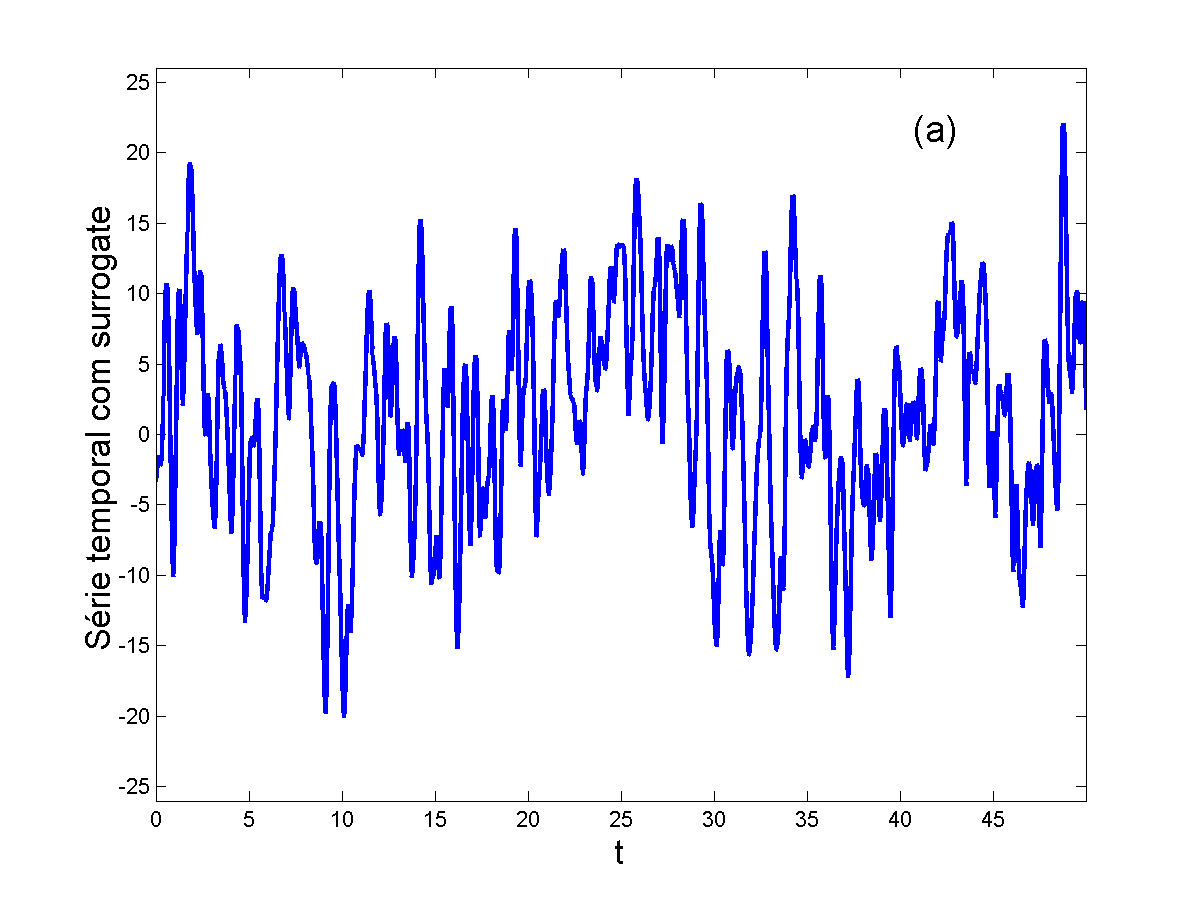
\includegraphics{Figuras/lorenzxsurr.png}} \resizebox{7.2cm}{!}{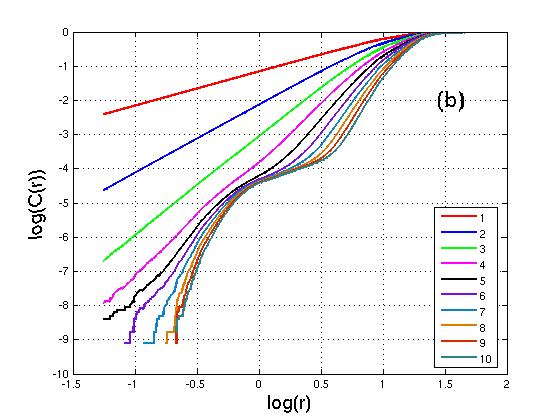
\includegraphics{Figuras/lorenzcorrelint2surr.png}} \\  \resizebox{7.2cm}{!}{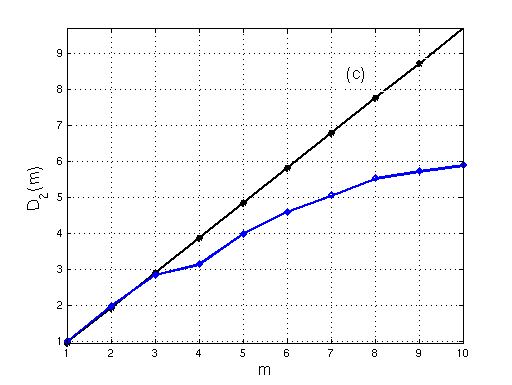
\includegraphics{Figuras/lorenzdimcorrelsurr2.png}} 
\caption{(a) S�rie temporal de Lorenz em $x$ com fase embaralhada. (b) Correla��o integral da s�rie em (a) com $m=1$ a $10$. (c) Dimens�o de correla��o da s�rie em (a) e dimens�o de correla��o infinita para uma s�rie aleat�ria}
\label{figlorenzsurrogate}
\end{figure}

Outro teste consiste em considerar a an�lise da correla��o integral~(\ref{eqcorr1}) da primeira derivada num�rica (ou primeira diferen�a) de uma s�rie temporal. Para um sistema governado por um atrator ca�tico de baixa dimens�o, o valor de $D_{2}$ � o mesmo tanto para a s�rie temporal original quanto para s�rie temporal modificada. Isto porque a primeira derivada num�rica (ou primeira diferen�a) mantem as correla��es existentes na s�rie original. 

A Figura~\ref{figlorenzdiff}(a) apresenta a primeira diferen�a $\Delta x(t)=x(t+\Delta t)-x(t)$ da componente $x$ do atrator de Lorenz, a Figura~\ref{figlorenzdiff}(b) apresenta a correla��o integral para $\Delta x$ e a Figura~\ref{figlorenzdiff}(c) apresenta os valores de $D_{2}$ associados. Foram feitas $5$ realiza��es an�logas � descrita acima, e a dimens�o de correla��o m�dia obtida foi de $D_{2}=\langle2.09\rangle$ com desvio padr�o de $\sigma_{D_{2}}=0.03$. Pode-se observar, neste caso, que a dimens�o de correla��o $D_{2}$ satura em um valor bastante pr�ximo daquela obtido com base na s�rie original. Este comportamento sugere mais uma vez a exist�ncia de uma din�mica de baixa dimens�o na s�rie temporal de Lorenz. Ainda, como $D_{2}\thickapprox 2.09$, pela rela��o de Takens dada por~(\ref{eqconditak}), o atrator de Lorenz pode ser bem representado em um espa�o de imers�o de $m=6$.

\begin{figure}[ht]
\centering 
\resizebox{7.2cm}{!}{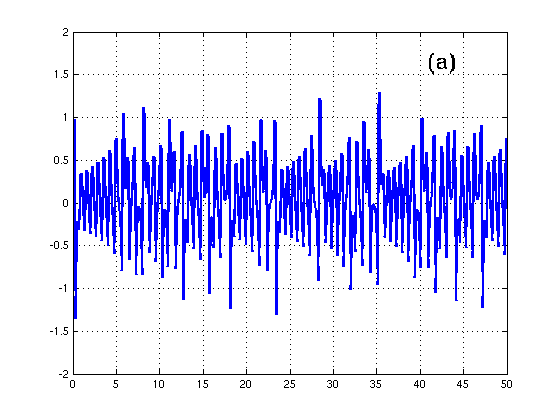
\includegraphics{Figuras/lorenzdiff2.png}} \resizebox{7.2cm}{!}{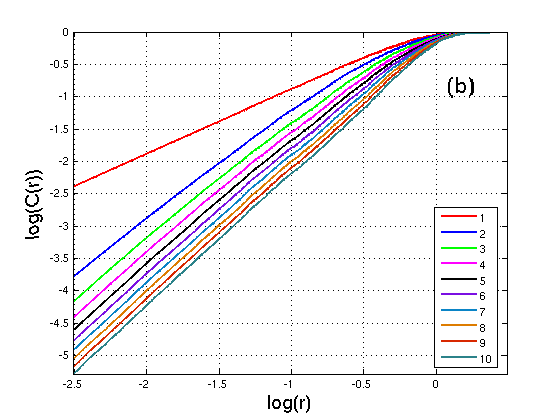
\includegraphics{Figuras/lorenzcorrelintdiff2.png}} \\  \resizebox{7.2cm}{!}{\includegraphics{Figuras/lorenzdimcorreldiff2.png}} 
\caption{(a) S�rie temporal gerada a partir da primeira diferen�a da s�rie temporal $x$ de Lorenz. (b) Correla��o integral da s�rie em (a) com $m=1$ a $10$. (c) Dimens�o de correla��o da s�rie em (a) e dimens�o de correla��o infinita para uma s�rie aleat�ria.}
\label{figlorenzdiff}
\end{figure}

A t�cnica de reconstru��o do espa�o de fase (\ref{eqtakensreconst}) como tamb�m o c�lculo da dimens�o de correla��o (\ref{eqcorr2}) devem ser usados ap�s uma avalia��o cuidadosa das condi��es de sua aplicabilidade, seguida de uma avalia��o da consist�ncia dos resultados obtidos. Uma aplica��o ing�nua de tais m�todos pode levar a conclus�es err�neas~\cite{osboproven/89}. \citeonline{eckruelllyap/92} fornecem evid�ncias segundo as quais o valor de $D_{2}$, estimado a partir do algoritmo de Grassberger-Procaccia, n�o fornece dimens�es confi�veis maiores que:

\begin{equation}
D_{2_{\textrm{max}}}=2\log_{10}N
\label{eqlimitemax}
\end{equation}
onde $N$ � o n�mero de pontos da s�rie temporal. Desta forma, quando o valor da dimens�o de correla��o satura em um valor superior ao estabelecido pela Equa��o~(\ref{eqlimitemax}) pode n�o ser correto afirmar a s�rie temporal possui uma din�mica de baixa dimens�o. Sob essa perspectiva, a dimens�o de correla��o obtida a partir de $10.000$ pontos da s�rie em $x$ de Lorenz � confi�vel j� que seu valor, a saber $D_{2}\thickapprox 2.1$, satisfaz a rela��o $D_{2_{\textrm{max}}}\leq 8$.

\subsubsection{Estacionaridade}
\label{subsecestacio}

O estudo das propriedades de um atrator associado a um sistema din�mico 
admite que o mesmo se encontre em um \textit{estado estacion�rio}\footnote{Sob o ponto de vista estat�stico, uma s�rie temporal � estacion�ria se a fun��o de densidade de probabilidade associada n�o se altera ao longo do tempo (estacionaridade plena), ou particularmente se os primeiros momentos associados a uma s�rie temporal, como m�dia e vari�ncia n�o se alteram ao longo do tempo (estacionaridade estrita).}, ou para o caso de um experimento real, muito pr�ximo desse estado - situa��o em que os pontos representativos da evolu��o temporal do sistema est�o bastante pr�ximos do atrator associado � din�mica. Desta forma, � importante verificar se a s�rie temporal em estudo corresponde, de fato, a um estado estacion�rio do sistema f�sico real~\cite{aguirre/00}.

O crit�rio de estacionaridade utilizada nesta disserta��o emprega janelas de dados deslizantes ao longo de uma s�rie. Ou seja, dada uma s�rie temporal~(\ref{eqserietemp}), pode-se definir como janelas de dados deslizantes todos os subconjuntos de amostras subseq�entes poss�veis, de comprimento $L$ (conforme Figura~\ref{figestaciogeral}). Testes que envolvem tais janelas procuram analisar e quantificar as propriedades que se alteram ao longo da s�rie temporal, como a m�dia e a vari�ncia, com base em um determinado intervalo de confian�a~\cite{alvaro/01}.

% \begin{figure}[ht]
% \centering \resizebox{15cm}{!}{\includegraphics{Figuras/figestacionaria.png}}
% \caption{Janelas de dados deslizantes} 
% \FONTE{\cite{alvaro/01}}
% \label{figestaciogeral}
% \end{figure}

\begin{figure}[!ht]
\begin{center}
\resizebox{12cm}{!}{\input{Figuras/estacionariaxfig2.pdftex_t}}
\caption{Janelas de dados deslizantes} 
\end{center}
\label{figestaciogeral}
\end{figure}
 
Desta forma, m�dias parciais ($\mu_{\textrm{parcial}}$) e vari�ncias parciais ($\sigma_{\textrm{parcial}}$) devem satisfazer as rela��es:
\begin{equation}
\begin{array}{rcccl}
\mu_{\textrm{total}}-\sigma_{\textrm{total}} & \leq  &  \mu_{\textrm{parcial}} & \leq  & \mu_{\textrm{total}}+\sigma_{\textrm{total}}\\
&   &   &   &\\
\sigma_{\textrm{total}}^2-\sigma_{\textrm{total}} & \leq  &  \sigma_{\textrm{parcial}}^2 & \leq  & \sigma_{\textrm{total}}^2+\sigma_{\textrm{total}}
\end{array}
\label{eqestacionaria}
\end{equation} 
onde $\mu_{\textrm{total}}$, $\sigma_{\textrm{total}}$ e $\sigma_{\textrm{total}}^2$ s�o a m�dia, desvio padr�o e vari�ncia da s�rie temporal, respectivamente.

O teste de estacionaridade descrito acima foi aplicado � s�rie $x$ de Lorenz com janelas deslizantes de comprimento $L=100$. Como todos os valores parciais de $\mu$ e $\sigma$ satisfazem a rela��o~(\ref{eqestacionaria}) pode-se dizer que tal s�rie � estacion�ria.


\subsubsection{Os expoentes de Lyapunov}

Em s�ries temporais experimentais, o ponto de partida para o c�lculo dos expoentes de Lyapunov � o atrator reconstru�do em uma dimens�o de imers�o $m$ adequada. Uma vez reconstru�do o atrator, define-se uma trajet�ria de refer�ncia (ou trajet�ria fiducial) a partir da seq��ncia de vetores reconstru�dos. Em seguida, deve-se analisar o que ocorre com pontos vizinhos desta trajet�ria. Com as informa��es sobre as taxas de diverg�ncia destes pontos, pode-se obter, ent�o, os expoentes de Lyapunov. 

Diversos m�todos t�m sido propostos para estimar esses expoentes em s�ries temporais experimentais~\cite{wolf/85,eckrue/86,sanosawada/85}. O m�todo proposto por \citeonline{wolf/85} permite calcular com expressiva precis�o o maior expoente de Lyapunov (positivo). Considere uma trajet�ria descrita pela seq��ncia de pontos $y(t_0), y(t_1), y(t_2),\cdots$ no atrator reconstru�do. Seja $z_0(t_0)$ o vizinho no atrator reconstru�do mais pr�ximo de $y(t_0)$ e $L_0$ a dist�ncia entre $y(t_0)$ e $z_0(t_0)$ (conforme Figura~\ref{figferraralyap}), isto �, $L_0=\left|y(t_0)-z_0(t_0)\right|<\epsilon$, e desta forma, $z_0(t_0)$ est� dentro da hiperesfera de raio $\epsilon$ centrada em $y(t_0)$. Acompanha-se ent�o a evolu��o temporal de $z_0$ e $y_0$ at� que num instante $t_1$ a dist�ncia entre esses pontos, $L_0{'}$, exceda $\epsilon$. Nesse momento substitui-se $z_0$ por um novo vizinho, mais pr�ximo de $y(t_1)$, que esteja na dire��o do segmento $L_0{'}$ e tal que $L_1=\left|y(t_1)-z_1(t_1)\right|<\epsilon$. O processo prossegue at� que todos os pontos $y(t_i)$ tenham sido percorridos. O maior expoente de Lyapunov positivo � obtido como a m�dia de $\log_{2} L_i{'}/L_i$, ao longo da trajet�ria de refer�ncia, isto �,

\begin{equation}
\lambda_{1}=\frac{1}{t_{M}-t_{0}}\sum_{i=0}^{M-1}\log_{2}\frac{L_i{'}}{L_i}
\label{lyap2}
\end{equation}
onde $M$ � o n�mero total de vezes que um novo vizinho foi escolhido pr�ximo � trajet�ria de refer�ncia.

\begin{figure}[ht]
\centering \resizebox{13cm}{!}{\includegraphics{Figuras/wolf.png}}
\caption{Representa��o esquem�tica do m�todo proposto por \citeonline{wolf/85}. O maior expoente de Lyapunov � estimado a partir da taxa de crescimento dos segmentos $L_i$. Quando o comprimento do segmento que liga dois pontos pr�ximos do atrator excede um certo valor $\epsilon$, um novo vizinho � escolhido de forma a minimizar o �ngulo $\theta_i$.}
\FONTE{Adaptada de \citeonline{wolf/85}}
\label{figferraralyap}
\end{figure}

Atrav�s do m�todo descrito acima � poss�vel obter uma aproxima��o num�rica para o maior expoente de Lyapunov, $\lambda_1$, calculado a partir da s�rie temporal em $x$ de Lorenz. Pode-se observar que a aproxima��o obtida � satisfat�ria j� que o maior expoente de Lyapunov, obtido diretamente do Sistema de EDO's (\ref{eqsistemalorenz}) � aproximadamente $2.16$ \cite{wolf/85}, enquanto que o obtido com base no algoritmo de \citeonline{wolf/85} � $2.18\pm0.01$.

\begin{figure}[ht]
\centering \resizebox{13cm}{!}{\includegraphics{Figuras/lorenzlyap3cond.png}}
\caption{Converg�ncia do maior expoente de Lyapunov ($\lambda_1$) associado � componente $x$ do atrator de Lorenz, com base no algoritmo desenvolvido por \citeonline{wolf/85}. A curva azul corresponde � condi��o inicial $(5,5,5)$, a curva vermelha corresponde � condi��o inicial $(5.01,5,5)$ e a curva preta corresponde � condi��o inicial $(5,10,5)$}
\label{figlorenzlyap}
\end{figure}

\subsection{Plots de Recorr�ncia}

A representa��o gr�fica bidimensional de uma matriz da forma:

\begin{equation}
R_{i,j}=\Theta(\varepsilon-\|\xi_{i}-\xi_{j}\|),\;\;\; i,j=1,\ldots,M
\label{eqplotrec}
\end{equation}

� definida como \textit{Plots de Recorr�ncia} (PR) e foi introduzida por \citeonline{eckmannplotrecorr/87}. Desta forma, $\xi_{i}\in\mathds{R}^m$ s�o vetores de dimens�o $m$ obtidos atrav�s da reconstru��o do espa�o de fase (\ref{eqtakensreconst}), $\varepsilon$ � um valor limite pr�-definido e $\Theta$ � uma fun��o degrau de Heavyside (conforme~\ref{eqheavyside}). Se a dist�ncia entre dois vetores $\xi_{i}$ e $\xi_{j}$ sobre a trajet�ria reconstru�da for menor que $\varepsilon$, a fun��o de Heavyside $\Theta$ assume o valor $1$, e neste caso a posi��o $(i,j)$ da matriz~(\ref{eqplotrec}) � representada por um ponto preto, caso contr�rio tal posi��o � representada por um ponto branco~\cite{eckmannplotrecorr/87,thielromano/04,thielemuitos/02,gaocai/00}.

Segundo \citeonline{eckmannplotrecorr/87} por meio de um PR � poss�vel visualizar o comportamento de trajet�rias no espa�o de fase~\cite{eckmannplotrecorr/87} e ainda um PR mostra todos os tempos no qual um estado de um sistema din�mico se repete. A repeti��o de estados � uma propriedade fundamental de um sistema din�mico determin�stico, e � um comportamento t�pico em sistemas ca�ticos ou n�o-lineares~\cite{thieltese/04}. 

Tradicionalmente, a visualiza��o de espa�os de fase com dimens�es maiores que $3$ � feita por meio de proje��es em sub-espa�os de dimens�o $2$ ou $3$. Contudo, um PR permite investigar a evolu��o de trajet�rias em um espa�o de fase com dimens�es elevadas por meio da representa��o bidimensional de suas repeti��es. 

A Figura~\ref{figrpsistemas} apresenta PRs para um sistema estoc�stico, um sistema peri�dico e um sistema determin�stico ca�tico. PRs associados � sistemas estoc�sticos freq�entemente apresentam uma certa homogeneidade em rela��o � distribui��o de seus pontos (conforme Figura~\ref{figrpsistemas}(a)). Sistemas que oscilam peri�dicamente apresentam estruturas de repeti��es peri�dicas cujas dist�ncias entre esses padr�es peri�dicos correspondem ao per�odo (conforme Figura~\ref{figrpsistemas}(b)). Sistemas din�micos ca�ticos possuem estruturas diagonais paralelas � diagonal principal (conforme Figura~\ref{figrpsistemas}(c)). Essas estruturas ocorrem quando um segmento da trajet�ria reconstru�da � paralelo � outro segmento, ou seja, a trajet�ria visita a mesma regi�o do espa�o de fase em diferentes tempos. O comprimento de tais estruturas � proporcional � dura��o da evolu��o local comum entre os segmentos da trajet�ria~\cite{thieltese/04,gaocai/00}.

\begin{figure}[ht]
\centering 
\resizebox{7.2cm}{!}{\includegraphics{Figuras/ruidorp.png}} \resizebox{7.2cm}{!}{\includegraphics{Figuras/senorp.png}} \\  \resizebox{7.2cm}{!}{\includegraphics{Figuras/lorenzrp.png}} 
\caption{(a) PR para um sistema estoc�stico (ru�do uniformemente distribu�do) com $m=1$ e $\varepsilon=0.09994$ . (b) PR para a fun��o seno com $m=1$ e $\varepsilon=0.2$. (c) PR correspondente � componente em $x$ do atrator de Lorenz com $m=6$ e $\varepsilon=4.9344$. O valor de $\varepsilon$ utilizados nos casos (a) e (b) correspondem � $10\%$ das vari�ncias associadas, e no caso (c) � $10\%$ do di�metro do espa�o de fase~\cite{thielromano/04}.}
\label{figrpsistemas}
\end{figure}

% \begin{figure}[ht]
% \centering 
% \resizebox{13cm}{!}{\includegraphics{Figuras/lorenzdet.png}\includegraphics{Figuras/lorenzembardet.png}}
% \caption{Atrator de Lorenz para o sistema~(\ref{eqsistemalorenzpart}). (a) Atrator original. (b) Atrator reconstru�do pelo m�todo das derivadas.}
% \label{lorenzdiff}
% \end{figure}

Uma das principais vantagens na aplica��o de um PR, em compara��o � aplica��o de t�cnicas de caracteriza��o de comportamento ca�tico tradicionais (como por exemplo o algoritmo de Grassberger e Procaccia~(\ref{eqcorr2})), � que o PR pode ser aplicado em s�ries temporais n�o estacion�rias e com poucos pontos~\cite{thieltese/04}. Uma desvantagem � que se o n�mero de pontos da s�rie temporal for muito grande (maior que 10.000 pontos), o n�mero de vetores reconstru�dos � tamb�m grande. Conseq�entemente, a ordem da matriz de dist�ncias~(\ref{eqplotrec}) se torna elevada. Este fato pode acarretar em insufici�ncia de mem�ria computacional na armazenagem desta matriz.



 % 3o capítulo
    %%%%%%%%%%%%%%%%%%%%%%%%%%%%%%%%%%%%%%%%%%%%%%%%%%%%%%%%%%%%%%%%%%%%%%%%%%%%%%%

\chapter{DADOS ANALISADOS}

Este capítulo aborda as características gerais da Região Amazônica. Apresenta-se a seguir a descrição e relevância do projeto LBA. Finalizando, é realizada a descrição dos dados coletados pela campanha WETAMC do projeto LBA, como também do sítio experimental, durante tal campanha.

\section{A Amazônia}
\label{sec:amazonia}

O bioma\footnote{Corresponde a certos padrões de clima, formações geológicas, relevo, solo, hidrografia, vegetação e biodiversidade, com características paisagísticas bem definidas.}Amazônia ocupa $50\%$ da superfície da América do Sul, toda a porção norte, distribuída por nove países. Essa região é limitada a oeste pela Cordilheira dos Andes (com elevações de até $6.000$ metros), ao norte pelo Planalto das Guianas (com picos montanhosos de até $3.000$ metros), ao sul pelo Planalto Central (com altitudes típicas de $1.200$ metros) e ao leste pelo Oceano Atlântico. Em território brasileiro está mais da metade dos $6,9$ milhões de quilômetros quadrados originalmente cobertos por floresta~\cite{fisch/98}. 

Segundo o IBGE, aproximadamente $60\%$ da Floresta Amazônica pertence ao território brasileiro, que compreende a Amazônia Legal\footnote{Em $1953$, a Constituição Federal criou o conceito político de ``Amazônia Legal'', que representa $61\%$ do território brasileiro. Além dos sete estados da região Norte, inclui o estado do Mato Grosso e cerca de $79\%$ do estado do Maranhão}. Os $40\%$ restantes estão distribuídos entre os países da Bolívia, Colômbia, Equador, Guiana, Guiana Francesa, Peru, Suriname e Venezuela. 

Parte da vegetação na Amazônia sofre grande influência do processo de subida e descida das águas, o chamado pulso hidrológico. As florestas inundáveis representam $5$ a $10\%$ da área da Amazônia. São definidas por estarem alagadas durante parte do tempo, diariamente, no caso dos manguezais, ou alguns meses por ano, no caso das várzeas e igapós, ou mesmo durante todo o ano, como nos pântanos. 

As florestas de terra firme representam mais de $80\%$ da área amazônica. Tais florestas estão livres de inundações, já que ocupam terras mais altas com altitudes médias de $200$ metros. Esse tipo de floresta apresenta árvores de grande porte, que variam de $30$ a $60$ metros em altura. O dossel retém cerca de $95\%$ dos raios solares, o que torna o interior da floresta úmido e escuro. 

A convecção na região amazônica é um importante mecanismo de aquecimento da atmosfera tropical e sua variação, em termos de intensidade e posição, possue um papel importante na determinação do tempo e do clima desta região~\cite{fisch/98}. O clima é, em geral, quente e úmido e o comportamento da temperatura do ar apresenta uma pequena variação ao longo do ano. A amplitude térmica sazonal é da ordem de $1$-$2\,^{\circ}$C, sendo que os valores médios situam-se entre $24\,^{\circ}$ e $28\,^{\circ}$C.

A precipitação é um dos elementos climáticos mais importantes a ser analisado na região tropical, pois induz as características e comportamento de variáveis tais como temperatura, umidade relativa, vento etc. A região amazônica possui uma precipitação média de aproximadamente $2.300$ mm.ano$^{-1}$. O período de chuvas ou forte atividade convectiva na região amazônica é compreendido entre novembro a março, sendo que o período de seca (sem grande atividade convectiva) ocorre entre os meses de maio e setembro. Os meses de abril e outubro são meses de transição entre um regime e outro~\cite{fisch/98}.

O conhecimento das diversas componentes envolvidas na interação entre a biosfera e a atmosfera é fundamental para a previsão da evolução do clima, da sustentabilidade do ecossistema como um todo, assim como para a tomada de decisão sobre as políticas públicas mais adequadas para a minimização de impactos danosos irreversíveis~\cite{silvadias/05}. 

 
\section{O projeto LBA}

Nas últimas décadas, vários experimentos micrometeorológicos têm sido realizados na região amazônica, com o objetivo de aumentar os conhecimentos relativos à interação entre a floresta tropical e a atmosfera. Dentre os experimentos realizados destaca-se a campanha micrometeorológica intensiva do Projeto LBA (Experimento de Grande Escala de Interação Biosfera-Atmosfera na Amazônia). 

O projeto LBA é um grande programa de pesquisas liderado pelo Brasil e com cooperação científica internacional, composto por mais de $130$ projetos de pesquisas (já executados ou em fase de execução), financiados por várias agências nacionais (como o MCT, o CNPQ, a FAPESP, a FINEP/PPG7, etc) e internacionais (com destaques para a NASA e a National Science Foundation, dos EUA, a Comissão Européia, o IAI - Instituto Interamericano de Pesquisas de Mudanças Globais, etc)~\cite{nobre/2005}. 

As duas questões centrais do LBA são: (i) como funciona a Amazônia, na forma de um sistema regional, com respeito aos ciclos da água, energia, carbono, gases do efeito estufa e nutrientes?; e (ii) como as mudanças de uso da terra e do clima podem afetar o funcionamento físico, químico e biológico dos ecossistemas amazônicos? Estas questões levam em conta que as mudanças climáticas e ambientais têm efeito sobre o uso sustentável dos recursos naturais e, de uma forma geral, sobre as populações. Deste modo, o LBA visa auxiliar na definição de critérios de uso sustentável da floresta e do solo da Amazônia~\cite{nobre/2005}. 

A Figura~\ref{mapalocal} apresenta um mapa esquemático com as áreas de pesquisa de campo do LBA. As áreas principais fazem parte de duas transeções ecofisiológicas e de usos da terra. As áreas secundárias de pesquisa serão estabelecidas em toda a Amazônia.

\begin{figure}[ht]
	\caption{Mapa esquemático com a localização das áreas de pesquisa de campo do projeto LBA.}
	\vspace{6mm}	% acrescentar o espaçamento vertical apropriado entre o título e a borda superior da figura
	\begin{center}
		\resizebox{10.5cm}{!}{\includegraphics{docs/figs/mapalbacorr.png}}		
	\end{center}
	\vspace{4mm}	% acrescentar o espaçamento vertical apropriado entre a borda inferior da figura e a legenda ou a fonte quando não há legenda (o valor pode ser negativo para subir)
	\legenda{Longitude em grau em abscisse e latitude em grau em ordenada.}	% legenda - para deixar sem legenda usar comando \legenda{} (nunca deve-se comentar o comando \legenda)
	\label{mapalocal}
	\FONTE{\citeonline{lba/06}.}	% fonte consultada (elemento obrigatório, mesmo que seja produção do próprio autor)
\end{figure}

\section{Sítio experimental e dados}
 
Os dados utilizados neste trabalho foram obtidos através de uma campanha micrometeorológica intensiva, a saber, WETAMC (Campanha de Mesoescala Atmosférica na Estação Úmida) que é parte do projeto LBA. Esta campanha foi realizada entre os meses de janeiro e março de 1999, na Reserva Biológica do Jaru ($10\,^{\circ}$46'S, $61\,^{\circ}$56'W), um sítio de floresta densa de aproximadamente $270$ mil hectares, pertencente ao Instituto Brasileiro do Meio Ambiente e dos Recursos Naturais Renováveis - IBAMA. Tal reserva está situada aproximadamente à $80$ Km ao norte de Ji-Paraná e a $120$ m acima do nível do mar, no estado de Rondônia, Brasil (ver Figura~\ref{rondonia}).  

\begin{figure}[ht]
	\caption{Mapa com a localização da campanha realizada pelo Projeto LBA.}
	\vspace{6mm}	% acrescentar o espaçamento vertical apropriado entre o título e a borda superior da figura
	\begin{center}
		\resizebox{11.5cm}{!}{\includegraphics{docs/figs/rondonia.pdf}}		
	\end{center}
		\vspace{2mm}	% acrescentar o espaçamento vertical apropriado entre a borda inferior da figura e a legenda ou a fonte quando não há legenda (o valor pode ser negativo para subir)
	\legenda{}	% legenda - para deixar sem legenda usar comando \legenda{} (nunca deve-se comentar o comando \legenda)
	\label{rondonia}
	\FONTE{\citeonline{iag/05}.}	% fonte consultada (elemento obrigatório, mesmo que seja produção do próprio autor)
\end{figure}

Uma estação meteorológica automática foi montada para medidas de resposta rápida de precipitação pluvial, temperatura do ar, umidade relativa do ar, velocidade e direção do vento, radiação solar incidente e de radiação de ondas longas emitida pela atmosfera e pela superfície, com médias coletadas em períodos de $30$ minutos, a uma freqüência de amostragem de $60$ Hz. Instrumentos como termômetros e anemômetros tridimensionais foram utilizados na área de floresta para medir tais variáveis meteorológicas e os fluxos de superfície (calor latente e calor sensível). 

As medidas foram feitas com o auxílio de uma torre micrometeorológica de alumínio de $66$ m de altura, simultaneamente em três diferentes alturas: Nível Superior ($66$ m - acima da copa); Nível Médio ($45$ m - no topo da copa); e Nível Inferior ($21$ m - abaixo da copa). 
A área onde tal torre foi construída está rodeada pela floresta amazônica de terra firme em um raio de pelo menos $800$ metros. As docs/figs~\ref{torre} e \ref{figtorre} mostram, respectivamente, um desenho esquemático da torre e as vistas superior e inferior da mesma. Maiores informações do sítio experimental podem ser encontradas em \citeonline{culf/96}.

\begin{figure}[ht]
	\caption{Desenho esquemático da torre micrometeorológica do projeto LBA.}
	\vspace{6mm}	% acrescentar o espaçamento vertical apropriado entre o título e a borda superior da figura
	\begin{center}
		\resizebox{14cm}{!}{\includegraphics{docs/figs/torredesenho.pdf}}		
	\end{center}
	\vspace{2mm}	% acrescentar o espaçamento vertical apropriado entre a borda inferior da figura e a legenda ou a fonte quando não há legenda (o valor pode ser negativo para subir)
	\legenda{}	% legenda - para deixar sem legenda usar comando \legenda{} (nunca deve-se comentar o comando \legenda)
	\label{torre}
	\FONTE{\citeonline{edtese/99}}.
\end{figure}

\begin{figure}[ht]
	\caption{Torre micrometeorológica de $66$ metros de altura construída na Reserva Biológica do Jaru (Rebio-Jaru), em Rondônia.}
	\vspace{6mm}	% acrescentar o espaçamento vertical apropriado entre o título e a borda superior da figura
	\begin{center}
		\resizebox{10.5cm}{!}{\includegraphics{docs/figs/2torres.pdf}}		
	\end{center}
	\vspace{2mm}	% acrescentar o espaçamento vertical apropriado entre a borda inferior da figura e a legenda ou a fonte quando não há legenda (o valor pode ser negativo para subir)
	\legenda{À esquerda, vista superior; à direita, vista inferior.}	% legenda - para deixar sem legenda usar comando \legenda{} (nunca deve-se comentar o comando \legenda)
	\FONTE{\citeonline{iag/05}}.
	\label{figtorre}
\end{figure}

Dois períodos de medidas distintos foram selecionados: às 12 horas, quando a copa da floresta é aquecida pelo sol e o topo da mesma é mais quente que os arredores, e desta forma a região acima da copa é instável; e às 23 horas, quando as condições são opostas, e a região acima da copa é estável~\cite{Ramos/04}. Durante o experimento, o estado da atmosfera foi caracterizado pela existência de uma forte atividade convectiva no período diurno, com eventos de chuvas isoladas de dia e à noite.

É importante destacar que os dados obtidos através desta campanha foram submetidos a um rigoroso controle de qualidade conforme \citeonline{bolzan/00}. Desta forma, problemas freqüentemente encontrados em sinais experimentais, como por exemplo picos espúrios e vales, foram removidos dos mesmos.
 % 4o capítulo
    %%%%%%%%%%%%%%%%%%%%%%%%%%%%%%%%%%%%%%%%%%%%%%%%%%%%%%%%%%%%%%%%%%%%%%%%%%%%%%%

\chapter{AN�LISE E RESULTADOS}
\label{capanaliseseresults}

A poss�vel natureza ca�tica da turbul�ncia na camada limite atmosf�rica, no interior e acima da copa da floresta � investigada. Com base na aplica��o de diversas ferramentas
%(j� descritas no Cap�tulo~\ref{caputiltecnicas}) 
nas s�ries temporais em estudo, o objetivo deste trabalho � determinar se tais s�ries incluem componentes determin�sticas que podem ser descritas (individualmente) por um sistema din�mico de baixa dimens�o, que se desenvolve em um atrator ca�tico.


\section{Estacionaridade}
Primeiramente, as s�ries temporais em estudo foram submetidas ao teste de estacionaridade.
% j� descrito na Se��o~\ref{subsecestacio}. 
A Tabela~\ref{tabelatempestacionaria} apresenta a classifica��o destas s�ries em estacion�rias ou n�o estacion�rias. Neste teste foram utilizadas janelas de dados deslizantes vari�veis, a saber, $L=100,500$ e $1000$. Desta forma, as an�lises subseq�entes ser�o feitas apenas com as s�ries do tipo estacion�rias.

\begin{table}[!ht]
\begin{center}
\caption{An�lise da estacionaridade para as s�ries temporais de temperatura e velocidade do vento em diferentes per�odos do dia e n�veis da copa.}
\begin{tabular}{c c c}
\hline 
\textbf{S�rie temporal} & \textbf{Estacionaridade} \\
\hline
tS1200 & estacion�ria \\
tI1200 & estacion�ria \\
tS2300 & n�o-estacion�ria \\
tI2300 & estacion�ria \\
tM1200 & estacion�ria \\
wS1200 & estacion�ria \\
tM2300 & n�o-estacion�ria \\
\hline
\end{tabular}
\label{tabelatempestacionaria}
\end{center}
\end{table}

\section{Decomposi��o dos Dados}

Com o objetivo de investigar o papel das estruturas coerentes na exist�ncia (ou n�o) de caos na atmosfera, decidiu-se selecionar dentre o conjunto de s�ries dispon�veis uma que apresentasse sinais n�tidos da presen�a de estruturas coerentes em rampa e em seguida decompor a mesma (denominada de s�rie total) em duas partes: uma parte dita coerente (baixas freq��ncias) e uma parte incoerente (altas freq��ncias). A parte coerente � caracterizada apenas pelas estruturas coerentes em rampa presentes na s�rie total, enquanto que a parte incoerente � caracterizada pelas flutua��es aparentemente aleat�rias da mesma s�rie. 

Desta forma, se a ocorr�ncia de uma din�mica de baixa dimens�o na s�rie temporal total estiver relacionada � presen�a de estruturas coerentes, � de se esperar que essa mesma din�mica se manifeste tamb�m na s�rie coerente, e que contrariamente, a s�rie incoerente esteja associada � uma din�mica de alta dimens�o. Por inspe��o visual, a s�rie escolhida para as an�lises subseq�entes corresponde �quela que apresenta estruturas coerentes em rampa, a saber, a s�rie de temperatura medida no n�vel superior da copa �s 12 horas (tS1200), conforme a parte superior da Figura~\ref{docs/figseriestempdiur}. 

%\subsection{Decomposi��o dos dados}

Inicialmente, a s�rie temporal total (tS1200) foi decomposta em suas partes coerente e incoerente, por meio da filtragem com Wavelet de Haar~\cite{katul/94}, que � um tipo de ondeleta-m�e discreta, definida por

\begin{equation}
\left\{ \begin{array}{rrr} 1, &  & 0\leq t < 1/2 \\
                  -1, &  & 1/2\leq t < 1 \\
		   0, &  & \mbox{caso contr�rio}
\end{array} 
\right.
\label{eqwavelethaar}
\end{equation} 

Esta categoria de ondaletas � utilizada para detectar varia��es bruscas nos sinais, e trabalha com sinais temporais que tenham comprimentos da ordem da pot�ncia de dois mais pr�xima, ou seja, $2^{f}=s$, onde $s$ � o comprimento total da s�rie, e $f$ � o n�mero de freq��ncias poss�veis para a decomposi��o. 

O comprimento da s�rie em estudo � de $s=108.000$ pontos. Desta forma, n�o h� um n�mero exato de decomposi��es em freq��ncias, j� que $f=16$ resulta em $s=65.536$ pontos e $f=17$ resulta em $s=131.072$ pontos. A estrat�gia utilizada foi completar o in�cio da s�rie temporal com zeros at� que a freq��ncia $f=17$ fosse alcan�ada. 
 
Ainda n�o h� na literatura um consenso de qual seja a melhor fun��o ondeleta a ser utilizada para a decomposi��o e filtragem de uma s�rie temporal. O que comumente se aceita � que a fun��o ondeleta possua um formato caracter�stico pr�ximo das caracter�sticas encontradas na s�rie temporal. Isso explica o fato da Wavelet de Haar ter sido escolhida para a decomposi��o da s�rie temporal de temperatura.  

A Figura~\ref{figfiltrotS0681200} mostra a s�rie temporal total, a s�rie temporal coerente (soma das baixas freq��ncias da s�rie total) e a s�rie temporal incoerente (soma das altas freq��ncias da s�rie total), respectivamente. Ap�s a filtragem da s�rie total, $23072$ pontos iniciais foram descartados das s�ries total, coerente e incoerente; tal valor corresponde ao n�mero de zeros inseridos na s�rie total antes do procedimento de filtragem. � importante ressaltar que a soma da s�rie coerente com a s�rie incoerente resulta a s�rie total, o que j� era esperado.

\begin{figure}[ht]
	\caption{S�ries temporal total, coerente e incoerente.}
	\vspace{0mm}	% acrescentar o espa�amento vertical apropriado entre o t�tulo e a borda superior da figura
	\begin{center}
		\resizebox{13cm}{!}{\includegraphics{docs/figs/filtrocoltS0681200.png}}		
	\end{center}
	\vspace{-2mm}	% acrescentar o espa�amento vertical apropriado entre a borda inferior da figura e a legenda ou a fonte quando n�o h� legenda (o valor pode ser negativo para subir)
	\legenda{Sinal total (superior), soma das nove primeiras freq��ncias (meio), soma das sete �ltimas freq��ncias (inferior).}	% legenda - para deixar sem legenda usar comando \legenda{} (nunca deve-se comentar o comando \legenda)
	\label{figfiltrotS0681200}
	\FONTE{Produ��o do autor.}	% fonte consultada (elemento obrigat�rio, mesmo que seja produ��o do pr�prio autor)
\end{figure}

\section{Caracterizando a turbul�ncia acima da copa da floresta Amaz�nica}

O objetivo desta se��o � verificar se as s�ries total, coerente e incoerente possuem as caracter�sticas t�picas da turbul�ncia plenamente desenvolvida, a saber, espectros de pot�ncia do tipo Kolmogorov e intermit�ncia nas pequenas escalas. Aproveita-se para ilustrar o papel crucial das estruturas coerentes no transporte de propriedades (quantidade de movimento, calor, etc.) atrav�s da copa da floresta.

\subsection{Espectros de pot�ncia}

Os espectros de pot�ncia das s�ries temporais total, coerente e incoerente foram estimados usando FFT (ver Figura~\ref{figespectrotS0681200}). Os resultados mostram que as inclina��es desses espectros no SI (em escala $\log$-$\log$) coincidem com a lei dos $-5/3$ de Kolmogorov. Esta observa��o demonstra que o fen�meno da turbul�ncia est� presente na s�rie total, o que era esperado, mas tamb�m nas s�ries coerente e incoerente. Em especial, pode-se afirmar que a s�rie incoerente est� mais relacionada � turbul�ncia de pequena escala do que a algum tipo de ru�do. Este comportamento � consistente com outros estudos que utilizaram a mesma abordagem de separa��o de um fluxo turbulento em uma parte coerente e outra incoerente~\cite{farge/01}.

\begin{figure}[ht]
	\caption{Espectros de pot�ncia das s�ries temporais total, coerente e incoerente.}
	\vspace{0mm}	% acrescentar o espa�amento vertical apropriado entre o t�tulo e a borda superior da figura
	\begin{center}
		\resizebox{15cm}{!}{\includegraphics{docs/figs/tS0681200espectro.png}\includegraphics{docs/figs/ctS0681200espectro.png}}\\ \resizebox{7.5cm}{!}{\includegraphics{docs/figs/itS0681200espectro.png}}		
	\end{center}
	\vspace{2mm}	% acrescentar o espa�amento vertical apropriado entre a borda inferior da figura e a legenda ou a fonte quando n�o h� legenda (o valor pode ser negativo para subir)
	\legenda{Em azul espectro de pot�ncia da s�rie temporal total, em vermelho da s�rie temporal coerente e em rosa da s�rie temporal incoerente. Observe que as inclina��es de todos os espectros no SI (em escala $\log$-$\log$) coincidem com a lei dos $-5/3$ de Kolmogorov. O espectro de pot�ncia associado a s�rie incoerente possui uma inclina��o adicional de $2.7$, que pode estar associada a um artefato num�rico.}	% legenda - para deixar sem legenda usar comando \legenda{} (nunca deve-se comentar o comando \legenda)
	\label{figespectrotS0681200}
	\FONTE{Produ��o do autor.}	% fonte consultada (elemento obrigat�rio, mesmo que seja produ��o do pr�prio autor)
\end{figure}

\subsection{Intermit�ncia}

A detec��o do fen�meno intermitente foi feita a partir das diferen�as das s�ries de temperatura total, coerente e incoerente (medida �s $12$ horas no n�vel superior) em v�rias escalas $r_{i}$ com $i=1,\ldots4$. Desta forma, as FDP's foram obtidas com base na distribui��o estat�stica das diferen�as $\Delta T_{r_{i}}=T(x+\Delta r_{i})-T(x)$. Os valores assumidos por $\Delta r_{i}$ s�o dados respectivamente por $1,10,100$ e $1000$, que para dados amostrados � $60$ Hz correspondem a $\Delta T_{t_{i}}$ de aproximadamente $0.0167,0.1667,1.6667$ e $16.6667$ segundos, respectivamente. % 5o capítulo
    %%%%%%%%%%%%%%%%%%%%%%%%%%%%%%%%%%%%%%%%%%%%%%%%%%%%%%%%%%%%%%%%%%%%%%%%%%%%%%%

\chapter{CONCLUSÕES}


Neste trabalho foi analisada a possível natureza caótica da turbulência atmosférica. Trata-se de uma questão ainda em aberto para a qual existem resultados discrepantes. As análises aqui realizadas, baseadas em dados de temperatura de alta resolução, obtidos pela campanha WETAMC do projeto LBA, sugerem a existência de um comportamento caótico de baixa dimensão na camada limite atmosférica. O atrator caótico correspondente possui uma dimensão de correlação de $D_{2}=3.50\pm0.05$. A presença de dinâmica caótica nos dados analisados é confirmada com a estimativa de um expoente de Lyapunov pequeno mas positivo, com valor $\lambda_{1}=0.050\pm0.002$. No entanto, esta dinâmica caótica de baixa dimensão está associada à presença das estruturas coerentes na camada limite atmosférica e não à turbulência atmosférica, como anteriormente afirmado por vários autores~\cite{xin/01,jaramillo/93,gallego/01}. Esta afirmação é evidenciada pelo processo de filtragem por wavelets utilizado nos dados experimentais estudados, que permite separar a contribuição da estruturas coerentes do sinal turbulento de fundo.

Este resultado corrobora a conjectura de \citeonline{loratrat/91}, que afirma que as ligações existentes entre caos e clima, apresentadas na literatura, decorrem não de erros de análise, mas da existência de subsistemas caóticos de baixa dimensão fracamente acoplados a um sistema maior, mais complexo e não caótico. No contexto deste trabalho, os subsistemas de baixa dimensão seriam as estruturas coerentes, comumente encontradas na camada limite, e o sistema maior, a atmosfera complexa e turbulenta. Os resultados obtidos neste trabalho, tanto para a dimensão de correlação $D_{2}$ quanto para o expoente de Lyapunov $\lambda_{1}$, são consistentes com valores publicados na literatura, onde evidências de atratores de baixa dimensão na atmosfera foram detectados~\cite{xin/01,jaramillo/93,gallego/01}. Apesar da presença de estruturas coerentes não ser explicitamente mencionada nestes trabalhos, uma leitura cuidadosa dos mesmos fornece indícios de que as séries temporais estudadas por esses autores possuem estruturas do tipo rampa, como as analisadas neste trabalho.
 
No plano computacional, esta dissertação ofereceu a oportunidade de estudar e implementar diversas ferramentas para o estudo de comportamento caótico em séries temporais. Apesar de populares, a maior parte destes algoritmos apresenta sérias dificuldades quando confrontados com o desafio de analisar séries ``reais'' (isto é, oriundas de sistemas dinâmicos naturais não conhecidos a priori), fracamente estacionárias, com muitos pontos (100 mil ou mais) e ainda por cima, contaminadas com ruído. Neste sentido, um resultado importante desta dissertação foi o desenvolvimento de uma ``cultura'' local, composta por adaptações, truques, etc., que permitiu ir além dos dados sintéticos e utilizar este tipo de série temporal. Esta ``cultura'' normalmente
permanece invisível na hora de relatar os resultados obtidos em uma pesquisa, mas é de fundamental importância para a realização de trabalhos futuros na área.

Finalmente, como linhas de pesquisa para trabalhos futuros sugere-se o desenvolvimento de um modelo dinâmico mínimo para descrever o comportamente das estruturas coerentes na copa da floresta, sob condições convectivas. Um modelo do tipo instabilidade de Kelvin-Helmholtz, que reconhecidamente apresenta propriedades caóticas~\cite{malik/92}, seria um bom ponto de partida. A análise de mais séries turbulentas que apresentem uma estrutura do tipo rampa, sob diferentes condições experimentais, é também uma continuação natural deste trabalho.
 % 6o capítulo
    ...
    \end{tcblisting}
\end{frame}

\begin{frame}[plain,fragile]{}
    \begin{tcblisting}{
        theorem={Listing}{listings}{Arquivo {\tt publicacao.tex} (Continuação)}{lst:example1},
        title=Arquivo {\tt publicacao.tex} (Continuação),
        fonttitle=\small\bfseries,
        center,width=0.92\paperwidth,
        colback=yellow!5,colframe=yellow!50!black
        listing engine=minted,
        minted language=latex,
        minted options={%
            linenos,
            breaklines,
            autogobble,
            fontsize=\small,
            numbersep=2mm,
            baselinestretch=1},
        overlay={%
        \begin{tcbclipinterior}
            \fill[gray!25] (frame.south west) rectangle ([xshift=4mm]frame.north west);
        \end{tcbclipinterior}},
        breakable, enhanced, listing only}
    ...
    % Bibliografia (obrigatório) 
    \bibliography{./bib/referencia} 
    
    %\include{./docs/glossario} 
    
    \inicioApendice % Opcional
    %%%%%%%%%%%%%%%%%%%%%%%%%%%%%%%%%%%%%%%%%%%%%%%%%%%%%%
%Ap�ndice A
\hypertarget{estilo:apendice1}{} %% uso para este Guia
%Este ap�ndice foi criado apenas para indicar como construir um ap�ndice no estilo, n�o existia no original da tese.
%%%%%%%%%%%%%%%%%%%%%%%%%%%%%%%%%%%%%%%%%%%%%%%%%%%%%%
\renewcommand{\thechapter}{}%
\chapter{AP�NDICE A - AUTORIZA��O PARA PUBLICA��O}	% trocar A por B na pr�xima ap�ndice e etc
\label{apendiceA}	% trocar A por B na pr�xima ap�ndice e etc
\renewcommand{\thechapter}{A}%		% trocar A por B na pr�xima ap�ndice e etc

H� dois formul�rios de autoriza��o para publica��o, um para publica��es de trabalhos acad�micos e outro para publica��es t�cnico-cient�ficas, neste ap�ndice encontram-se os modelos dos formul�rios e suas respectivas instru��es de preenchimento. 

\section{Autoriza��o para Publica��o de Trabalho Acad�mico - INPE-393}

\label{instr393}

	\begin{figure}[ht]
		\caption{Formul�rio Autoriza��o para Publica��o de Trabalho Acad�mico INPE-393.}
		\vspace{6mm}	% acrescentar o espa�amento vertical apropriado entre o t�tulo e a borda superior da figura
		\centering
   		\includegraphics[height=16cm]{./figs/form393.png}	   
 		\label{form393}
	\end{figure}


\subsection{Instru��es do Formul�rio INPE-393} 

\begin{enumerate} 

 \item \textbf{s�rie:} com este n�mero o SID identifica as publica��es do INPE, composto da sigla da Institui��o, n�mero sequencial geral da publica��o, sigla e n�mero sequencial do tipo de publica��o, exemplo: INPE-14209-TDI/1110;
 
 \item \textbf{n�mero:} ser� composto da sigla da unidade do SID, mais 4 (quatro) d�gitos e do ano em curso. Este n�mero de refer�ncia � de controle da unidade emissora. Ex.: SID-0001/2007;

 \item \textbf{t�tulo da publica��o:} deve ser completo, evitando-se abreviar palavras;

 \item \textbf{nome do autor e do orientador:} estes campos devem ser preenchidos por extenso, da mesma forma em que ir�o constar da publica��o;

 \item \textbf{origem da publica��o:} sigla da unidade do servidor (autor da publica��o), conforme TQ-001;

 \item \textbf{curso:} sigla do curso, de acordo com a Estrutura de Divis�o de Trabalho - EDT do INPE;
 
 \item \textbf{tipo:} assinalar se � tese ou disserta��o;

 \item \textbf{apresenta��o:} colocar a data de aprova��o final;

 \item \textbf{revis�o t�cnica:} o respons�vel designado pela Banca Examinadora para verifica��o de corre��es e, na aus�ncia desse, o orientador da tese ou disserta��o deve
carimbar, datar e assinar ap�s a vers�o \emph{on line} do trabalho;

 \item \textbf{revis�o de linguagem:} o respons�vel designado pela Banca Examinadora para verifica��o de corre��es, e na aus�ncia deste o orientador deve assinalar a solicita��o ou a dispensa da revis�o de linguagem e, carimbar, datar e assinar; o revisor deve datar e assinar ap�s a revis�o;
 
 \item \textbf{distribui��o:} O SID deve informar a quantidade de CD's e de c�pias impressas da tese ou disserta��o, conforme lista de distribui��o;
 
 \item \textbf{verifica��o de normaliza��o:}  Ap�s a verifica��o da vers�o \emph{on line} do trabalho quanto �s normas editoriais, o SID deve datar e assinar;
 
 \item \textbf{autoriza��o final:} data e assinatura do Titular de N�vel A, conforme TQ-001, a que o Servi�o de P�s-Gradua��o estiver subordinado.
 
 \item \textbf{observa��es:} para outras informa��es necess�rias. 

\end{enumerate}

\section{Autoriza��o para Publica��o - INPE-106}
\begin{figure}[h!]
	\caption{Formul�rio Autoriza��o para Publica��o de Trabalho Acad�mico INPE-106 folha 1.} 
	\vspace{6mm}	% acrescentar o espa�amento vertical apropriado entre o t�tulo e a borda superior da figura
	\centering
	\includegraphics[height=18cm]{./figs/form106.png}
	\label{form106}
\end{figure}

\begin{figure}[h!]
	\caption{Formul�rio Autoriza��o para Publica��o de Trabalho Acad�mico INPE-106 folha 2.} 
	\vspace{6mm}	% acrescentar o espa�amento vertical apropriado entre o t�tulo e a borda superior da figura
	\centering
	\includegraphics[height=18cm]{./figs/form106folha2.png}
	\label{form106a}
\end{figure}

\clearpage
\subsection{Instru��es do Formul�rio INPE-106} 
\label{instr106}


\begin{enumerate}

 \item \textbf{s�rie:} com este n�mero o SID identifica as publica��es do INPE, composto da sigla da Institui��o, n�mero sequencial geral da publica��o, sigla e n�mero sequencial do tipo de publica��o, exemplo: INPE-5616-RPQ/671. 
 
 \item \textbf{n�mero:} ser� composto da sigla da unidade constante da Estrutura Organizacional do INPE (TQ-001), mais 4 (quatro) d�gitos e do ano em curso. Este n�mero de refer�ncia � de controle da unidade solicitante. Ex: CEA-0001/2007;
 
 \item \textbf{t�tulo da publica��o:} deve ser completo, evitando-se abreviar palavras;

 \item \textbf{nome do autor, tradutor e editor:}  estes campos devem ser preenchidos por extenso, da mesma forma em que ir�o constar da publica��o;

 \item \textbf{origem da publica��o:} sigla da unidade do servidor (autor da publica��o), conforme TQ-001;

 \item \textbf{projeto:} sigla do projeto de acordo com a Estrutura de Divis�o de Trabalho - EDT do INPE;

 \item \textbf{tipo de publica��o:} assinalar o tipo de publica��o proposta:

 \begin{enumerate}
  \item{Rel�torio de Pesquisa (RPQ)},
  \item{Notas T�cnico-Cient�ficas (NTC)},
  \item{Propostas e Relat�rios de de Projeto (PRP)},
  \item{Manuais T�cnicos (MAN)},
  \item{Publica��es Did�ticas (PUD)},
  \item{Trabalhos Acad�micos Externos (TAE)}.
 \end{enumerate}

 \item \textbf{divulga��o:} assinalar, de acordo com os crit�rios de classifica��o. Se houver Lista de Divulga��o, nesta dever� constar os nomes e endere�os completos;

 \item \textbf{conv�nio:} descrever o nome da institui��o, quando a publica��o for realizada pelo INPE e outra organiza��o, preencher somente para o tipo PRP; 
 
    \item \textbf{autoriza��o preliminar:} data, carimbo e assinatura do Titular da Unidade a que o autor esteja subordinado e, assinatura do revisor que efetuou a revis�o t�cnica aprovando a vers�o \emph{on line} do trabalho e do revisor que realizou a revis�o de linguagem, quando solicitadas; 
    
  \item \textbf{verifica��o de normaliza��o:} o SID deve datar e assinar ap�s a revis�o da adequa��o �s normas editoriais;   
  
  \item \textbf{distribui��o:} O SID deve informar a quantidade de CD's e de c�pias impressas que dever�o ser gravados conforme lista de distribui��o;
  
 \item \textbf{autoriza��o final:} data, carimbo e assinatura do Titular de N�vel "A", conforme TQ-001, a que o autor da publica��o estiver subordinado;
 
 \item \textbf{observa��es:} para outras informa��es necess�rias, inclusive para descrever as justificativas de uma publica��o.
\end{enumerate} 
    
    \inicioAnexo
    %%%%%%%%%%%%%%%%%%%%%%%%%%%%%%%%%%%%%%%%%%%%%%%%%%%%%%
%Anexo
%Este anexo foi incluido para explicar como incluir um anexo no estilo, n�o existia no original desta tese.
%%%%%%%%%%%%%%%%%%%%%%%%%%%%%%%%%%%%%%%%%%%%%%%%%%%%%%%%%%%%%%%%%%%%%%%%%%%%%%%%%
\renewcommand{\thechapter}{}%
\chapter{ANEXO A - ABREVIATURA DOS MESES} %% T�tulo do anexo sempre em mai�sculas. Trocar A por B no pr�ximo anexo e etc
\label{anexoA} %% R�tulo aplicado caso queira referir-se a este t�pico em qualquer lugar do texto. Trocar A por B no pr�ximo anexo e etc
\renewcommand{\thechapter}{A}%		% trocar A por B no pr�ximo anexo e etc

\begin{table}[!ht]
 \label{tab:abreviaturas}
  \begin{center}
 	\begin{tabular}{lll}
	 \hline
	  \textbf{Portugu�s}    & \textbf{Espanhol}  & \textbf{Italiano}\\ 
   \hline
       janeiro   = jan.   & enero = ene.       & gennaio = gen.\\
       fevereiro = fev.   & febrero = feb.     & febbraio = feb.\\
       mar�o     = mar.   & marzo = mar.       & marzo = mar.\\
       abril     = abr.   & abril = abr.       & aprile = apr.\\
       maio      = maio   & mayo = mayo        & maggio = mag.\\ 
       junho     = jun.   & junio = jun.       & giugno = giu.\\ 
       julho     = jul.   & julio = jul.       & luglio = lug.\\
       agosto    = ago.   & agosto = ago.      & agosto = ago.\\
       setembro  = set.   & septiembre = sep.  & settembre = set.\\
       outubro   = out.   & octubre = oct.     & ottobre = ott.\\
       novembro  = nov.   & noviembre =nov.    & novembre = nov.\\
       dezembro  = dez.   & diciembre = dic.   & dicembre = dic.\\ 
     \hline
   \textbf{Franc�s}       & \textbf{Ingl�s}    & \textbf{Alem�o}\\
     \hline
       janvier = jan.     & January = Jan.     & Januar = Jan.\\
       f�vrier = f�v.     & February = Feb.    & Februar = Feb.\\
       mars = mars        & March = Mar.       & M�rz = M�rz\\
       avril = avr.       & April = Apr.       & April = Apr.\\
       mai = mai          & May = May          & Mai = Mai.\\
       juin = juin        & June = June        & Juni = Juni\\
       juillet = juil.    & July = July        & Juli = Juli\\
       ao�t = ao�t        & August = Aug.      & August = Aug.\\
       septembre = sept.  & September = Sept.  & September = Sept.\\
       octobre = oct.     & October = Oct.     & Oktober = Okt.\\
       novembre = nov.    & November = Nov.    & November = Nov.\\
       d�cembre = d�c.    & December = Dec.    & Dezember = Dez. \\ 
    \hline
   \end{tabular}
   \end{center}
	 \FONTE{Adaptada de \citeonline[p.~22]{NBR6023:2002b}.}
\end{table}
    %%%%%%%%%%%%%%%%%%%%%%%%%%%%%%%%%%%%%%%%%%%%%%%%%%%%%%%
%Anexo
%Este anexo foi incluido para explicar como incluir um anexo no estilo, não existia no original desta tese
%exceto algumas tabelas que foram modificadas
%%%%%%%%%%%%%%%%%%%%%%%%%%%%%%%%%%%%%%%%%%%%%%%%%%%%%%%%%%%%%%%%%%%%%%%%%%%%%%%%%
\renewcommand{\thechapter}{}%
\chapter{ANEXO B - EXEMPLOS DE FIGURAS E TABELAS NO \LaTeX} %% Título do anexo sempre em maiúsculas.
\label{anexoB} %% Rótulo aplicado caso queira referir-se a este tópico em qualquer lugar do texto.
\renewcommand{\thechapter}{B}%

\section{docs/figs} %% Título de secção sempre com as primeiras letras em maiúsculas.
\label{anexo2}

\begin{figure}[ht]
	\caption{Exemplo de figura com título curto.}
	\vspace{6mm}	% acrescentar o espaçamento vertical apropriado entre o título e a borda superior da figura
	\begin{center}
    	\includegraphics[width=\mylenfig]{./docs/figs/gpa.pdf}  
	\end{center}
	\vspace{4mm}	% acrescentar o espaçamento vertical apropriado entre a borda inferior da figura e a legenda ou a fonte quando não há legenda (o valor pode ser negativo para subir)
	\legenda{Exemplo de legenda curta.}	% legenda - opcional
	\label{figgpa1}
	\FONTE{\citeonline{lba/06}.}	% fonte consultada (elemento obrigatório, mesmo que seja produção do próprio autor)
\end{figure}

\begin{figure}[!h]
	\caption{Figura com título que ocupa mais de uma linha, alinhar as demais com a primeira
letra depois do hífen.}
%o ajuste do título é feito automaticamente pelo \LaTeX\ caso este ocupe mais de uma linha.}
	\vspace{6mm}	% acrescentar o espaçamento vertical apropriado entre o título e a borda superior da figura
	\begin{center}
    	\includegraphics[width=\mylenfig]{./docs/figs/gpa.pdf}  
	\end{center}
	\vspace{4mm}	% acrescentar o espaçamento vertical apropriado entre a borda inferior da figura e a legenda ou a fonte quando não há legenda (o valor pode ser negativo para subir)
	\legenda{Exemplo de legenda que ocupa mais de uma linha, alinhar as demais com a primeira
letra da primeira linha.}	% legenda - opcional
%o \LaTeX\ alinha o texto automaticamente.
	\label{figgpa2}
	\FONTE{Se o texto da fonte for longo e ocupar mais de uma linha as demais ficam alinhadas
	com a palavra fonte. Adaptada de \citeonline{mauri:2003}.}	% fonte consultada (elemento obrigatório, mesmo que seja produção do próprio autor)
%o \LaTeX\ alinha o texto automaticamente.
\end{figure}

\clearpage
\section{Tabelas} 

\begin{table}[!ht]%[htbp] %opções de colocação da tabela no texto
  \begin{center}	% use sempre um ambiente para as tabelas
									% (opções: center (recomendado), flushright, flushleft)
									% NÃO USE \centering com TABELAS se houver \FONTE!	
  \caption{Exemplo de tabela, com fonte.}
    \begin{tabular}{l|l|c|c|r|r}
			\hline % desenha uma linha horizontal
				Campo 1 & Campo2 & Campo3 & Campo 4 & Campo5 & Campo6 \\
				Campo 1 & Campo2 & Campo3 & Campo 4 & Campo5 & Campo6 \\
				Campo 1 & Campo2 & Campo3 & Campo 4 & Campo5 & Campo6 \\				
			\hline % desenha uma linha horizontal
    \end{tabular}
    \end{center}
 \FONTE{Coloque a fonte de referência aqui, se houver.}
\end{table}

% \hhline{|--|} \multicolumn{2}{|c|}{continuação da página anterior} \\
% \hhline{|--|} \endhead % ate aqui eh definicao do "head" da pagina 
%   % dois em diante
% \hhline{|--|} \multicolumn{2}{|c|}{continua para próxima página} \\
% \hhline{|--|} \endfoot % ate aqui eh definicao do "foot" exceto ultima página
% \hhline{|b:=:=:b|} \endlastfoot % ate aqui eh definicao do "foot" 
%   % da ultima pagina

\begin{table}[hb]
\renewcommand{\baselinestretch}{1.4}% for tabular environment
\small
   \centering
   \caption{Exemplo de tabela, com fonte longa}
%   \label{\fullpaperid:table:1}% you must prefix your labels (here table:1) with the string \fullpaperid: (this will be important when combining all the full papers for the final book)
	\begin{center}
	   \begin{tabular}{lcc}
	       \hline% horizontal line
	       \itshape Parameter&
	           \itshape $\kappa$ Scaling&
	           \itshape $\kappa$, $\lambda$ Scaling\\*
	       \hline
	       Dimension&
	           $\kappa^{-1}$&
	           $\lambda^{-1}$\\*
	       Currant&
	           $\kappa^{-1}$&
	               $\lambda/\kappa^{2}$\\*
	       Dopant Concentration&
	           $\kappa$&
	           $\lambda2/\kappa$\\*
	       \hline
	   \end{tabular}
	\end{center}
    \renewcommand{\baselinestretch}{1.0}
    \FONTE{Coloque a fonte longa longa longa longa longa longa longa longa longa longa aqui, se houver.}
\end{table}

% Exemplos de 2 tabelas avançadas 

\begin{table}[ht!]
\caption{Outro exemplo de tabela}
%\label{\fullpaperid:table:2}
\begin{center}
\renewcommand{\baselinestretch}{1.2}% for tabular environment
\small
\begin{tabular}{cccccc}
\hline
   & \multirow{2}{22mm}{\renewcommand{\baselinestretch}{0.7}\small\centering Quantitative measures} & \multicolumn{4}{c}{Markers} \\ \cline{3-6}
   & & \multicolumn{1}{c}{RO} & \multicolumn{1}{c}{ASF} & \multicolumn{1}{c}{ISO} & \multicolumn{1}{c}{ADF} \\ \hline
   \multirow{3}{20mm}{\renewcommand{\baselinestretch}{0.7}\small\centering Test image scale 2}
& RMSE & 0.126 & 0.187 & 0.118 & 0.103 \\
& NMSE & 0.046 & 0.101 & 0.040 & 0.031 \\
& SSIM & 0.9981 & 0.9956 & 0.9984 & 0.9989 \\ \hline
   \multirow{3}{18mm}{\renewcommand{\baselinestretch}{0.7}\small\centering Cameraman scale 4}
& RMSE & 13.748 & 15.649 & 10.132 & 4.325 \\
& NMSE & 0.011 & 0.014 & 0.006 & 0.001 \\
& SSIM & 0.923 & 0.847 & 0.904 & 0.933 \\ \hline
   \multirow{3}{18mm}{\renewcommand{\baselinestretch}{0.7}\small\centering Cameraman scale 7}
& RMSE & 20.963 & 22.652 & 13.108 & 4.650 \\
& NMSE & 0.024 & 0.029 & 0.010 & 0.001 \\
& SSIM & 0.851 & 0.757 & 0.866 & 0.925 \\ \hline
   \multirow{3}{23mm}{\renewcommand{\baselinestretch}{1.2}\small\centering Crop of cameraman scale 7}
& RMSE & 30.914 & 31.943 & 17.831 & 2.870 \\
& NMSE & 0.053 & 0.057 & 0.018 & 0.001 \\
& SSIM & 0.831 & 0.772 & 0.891 & 0.983 \\ \hline
\end{tabular}
\end{center}
\end{table}

\begin{table}[ht!]
\caption{Mais um exemplo de tabela}
%\label{\fullpaperid:table:1}
\begin{center}
\renewcommand{\baselinestretch}{1.2}% for tabular environment
\small
\begin{tabular}{ccccc}
\hline
\multirow{4}{16mm}{\renewcommand{\baselinestretch}{0.7}\small\centering Leveling's Scale} & \multicolumn{4}{c}{Values for the scale relation of the four different type of markers} \\ \cline{2-5}
& \multirow{3}{29mm}{\renewcommand{\baselinestretch}{1}\small\centering Structure element's size $r$ for RO and ASF} & \multicolumn{2}{c}{Isotropic diffusion} & \multirow{3}{20mm}{\renewcommand{\baselinestretch}{1}\small\centering Anisotropic diffusion iterations $t$} \\ \cline{3-4}
& & \multirow{2}{23mm}{\renewcommand{\baselinestretch}{0.7}\small\centering Standard deviation $\sigma$} & \multirow{2}{12mm}{\renewcommand{\baselinestretch}{0.7}\small\centering Kernel size} & \\
& & & & \\ \hline
1 & 1 & 0.5 & $5 \times 5$ & 100 \\
2 & 2 & 1.0 & $7 \times 7$ & 200 \\
3 & 3 & 1.5 & $11 \times 11$ & 300 \\
4 & 4 & 2.0 & $13 \times 13$ & 400 \\
5 & 5 & 2.5 & $17 \times 17$ & 500 \\
6 & 6 & 3.0 & $19 \times 19$ & 600 \\
7 & 7 & 3.5 & $23 \times 23$ & 700 \\ \hline
\end{tabular}
\end{center}
\end{table} 

\setlongtables
\begin{longtable}[c]{c|c|c|c|c|c}
\caption{Exemplo de tabela longa que atravessa várias páginas.}\label{tab:longas}\\
\hline
\textbf{Campo1} & \textbf{Campo2} & \textbf{Campo3} & \textbf{Campo4} & \textbf{Campo5} & \textbf{Campo6} \\
\hline\hline
\endfirsthead
\caption[]{Continuação} \\
\hline
\textbf{Campo1} & \textbf{Campo2} & \textbf{Campo3} & \textbf{Campo4} & \textbf{Campo5} & \textbf{Campo6} \\
\hline\hline
\endhead
\hline\hline
\endlastfoot
\hline
\multicolumn{6}{r}{\captionlabelfont\captionsize(Continua)}\\
\endfoot


	campo1 & campo2 & campo3 & campo4 & campo5 & campo6 \\
	campo1 & campo2 & campo3 & campo4 & campo5 & campo6 \\
	campo1 & campo2 & campo3 & campo4 & campo5 & campo6 \\
	campo1 & campo2 & campo3 & campo4 & campo5 & campo6 \\
	campo1 & campo2 & campo3 & campo4 & campo5 & campo6 \\
	campo1 & campo2 & campo3 & campo4 & campo5 & campo6 \\
	campo1 & campo2 & campo3 & campo4 & campo5 & campo6 \\
	campo1 & campo2 & campo3 & campo4 & campo5 & campo6 \\
	campo1 & campo2 & campo3 & campo4 & campo5 & campo6 \\
	campo1 & campo2 & campo3 & campo4 & campo5 & campo6 \\
	campo1 & campo2 & campo3 & campo4 & campo5 & campo6 \\
	campo1 & campo2 & campo3 & campo4 & campo5 & campo6 \\
	campo1 & campo2 & campo3 & campo4 & campo5 & campo6 \\
	campo1 & campo2 & campo3 & campo4 & campo5 & campo6 \\
	campo1 & campo2 & campo3 & campo4 & campo5 & campo6 \\
	campo1 & campo2 & campo3 & campo4 & campo5 & campo6 \\
	campo1 & campo2 & campo3 & campo4 & campo5 & campo6 \\
	campo1 & campo2 & campo3 & campo4 & campo5 & campo6 \\
	campo1 & campo2 & campo3 & campo4 & campo5 & campo6 \\
	campo1 & campo2 & campo3 & campo4 & campo5 & campo6 \\
	campo1 & campo2 & campo3 & campo4 & campo5 & campo6 \\
	campo1 & campo2 & campo3 & campo4 & campo5 & campo6 \\
	campo1 & campo2 & campo3 & campo4 & campo5 & campo6 \\
	campo1 & campo2 & campo3 & campo4 & campo5 & campo6 \\
	campo1 & campo2 & campo3 & campo4 & campo5 & campo6 \\
	campo1 & campo2 & campo3 & campo4 & campo5 & campo6 \\
	campo1 & campo2 & campo3 & campo4 & campo5 & campo6 \\
	campo1 & campo2 & campo3 & campo4 & campo5 & campo6 \\
	campo1 & campo2 & campo3 & campo4 & campo5 & campo6 \\
	campo1 & campo2 & campo3 & campo4 & campo5 & campo6 \\
	campo1 & campo2 & campo3 & campo4 & campo5 & campo6 \\
	campo1 & campo2 & campo3 & campo4 & campo5 & campo6 \\
	campo1 & campo2 & campo3 & campo4 & campo5 & campo6 \\
	campo1 & campo2 & campo3 & campo4 & campo5 & campo6 \\
	campo1 & campo2 & campo3 & campo4 & campo5 & campo6 \\
	campo1 & campo2 & campo3 & campo4 & campo5 & campo6 \\
	campo1 & campo2 & campo3 & campo4 & campo5 & campo6 \\
	campo1 & campo2 & campo3 & campo4 & campo5 & campo6 \\
	campo1 & campo2 & campo3 & campo4 & campo5 & campo6 \\
	campo1 & campo2 & campo3 & campo4 & campo5 & campo6 \\
	campo1 & campo2 & campo3 & campo4 & campo5 & campo6 \\
	campo1 & campo2 & campo3 & campo4 & campo5 & campo6 \\
	campo1 & campo2 & campo3 & campo4 & campo5 & campo6 \\
	campo1 & campo2 & campo3 & campo4 & campo5 & campo6 \\
	campo1 & campo2 & campo3 & campo4 & campo5 & campo6 \\
	campo1 & campo2 & campo3 & campo4 & campo5 & campo6 \\
	campo1 & campo2 & campo3 & campo4 & campo5 & campo6 \\
	campo1 & campo2 & campo3 & campo4 & campo5 & campo6 \\
	campo1 & campo2 & campo3 & campo4 & campo5 & campo6 \\
	campo1 & campo2 & campo3 & campo4 & campo5 & campo6 \\
	campo1 & campo2 & campo3 & campo4 & campo5 & campo6 \\
	campo1 & campo2 & campo3 & campo4 & campo5 & campo6 \\
	campo1 & campo2 & campo3 & campo4 & campo5 & campo6 \\
	campo1 & campo2 & campo3 & campo4 & campo5 & campo6 \\
	campo1 & campo2 & campo3 & campo4 & campo5 & campo6 \\
	campo1 & campo2 & campo3 & campo4 & campo5 & campo6 \\
	campo1 & campo2 & campo3 & campo4 & campo5 & campo6 \\
	campo1 & campo2 & campo3 & campo4 & campo5 & campo6 \\
	campo1 & campo2 & campo3 & campo4 & campo5 & campo6 \\
	campo1 & campo2 & campo3 & campo4 & campo5 & campo6 \\
	campo1 & campo2 & campo3 & campo4 & campo5 & campo6 \\
	campo1 & campo2 & campo3 & campo4 & campo5 & campo6 \\
	campo1 & campo2 & campo3 & campo4 & campo5 & campo6 \\
	campo1 & campo2 & campo3 & campo4 & campo5 & campo6 \\
	campo1 & campo2 & campo3 & campo4 & campo5 & campo6 \\
	campo1 & campo2 & campo3 & campo4 & campo5 & campo6 \\
	campo1 & campo2 & campo3 & campo4 & campo5 & campo6 \\
	campo1 & campo2 & campo3 & campo4 & campo5 & campo6 \\
	campo1 & campo2 & campo3 & campo4 & campo5 & campo6 \\
	campo1 & campo2 & campo3 & campo4 & campo5 & campo6 \\
	campo1 & campo2 & campo3 & campo4 & campo5 & campo6 \\
	campo1 & campo2 & campo3 & campo4 & campo5 & campo6 \\
	campo1 & campo2 & campo3 & campo4 & campo5 & campo6 \\
\hline
\end{longtable}
% o comando \FONTE{} não pode ser usado neste caso
\vspace{-8mm}
\begin{center}
	Fonte: Referência a fonte da tabela.
\end{center}


A \autoref{tab:longa} é um exemplo de tabela no modo paisagem e que ocupa também várias páginas.

\setlongtables
\begin{landscape}
\begin{longtable}[c]{c|c|c|c|c|c|c|c|c|c}
\caption{Exemplo de tabela longa, em paisagem, que atravessa várias páginas.}\label{tab:longa}\\
\hline
\textbf{BOX1} & \textbf{BOX2} & \textbf{BOX3} & \textbf{BOX4} & \textbf{BOX5} & \textbf{BOX6} & \textbf{BOX7} & \textbf{BOX8} & \textbf{BOX9} & \textbf{BOX10} \\
\hline\hline
\endfirsthead
\caption[]{Conclusão}\\
\hline
\textbf{BOX1} & \textbf{BOX2} & \textbf{BOX3} & \textbf{BOX4} & \textbf{BOX5} & \textbf{BOX6} & \textbf{BOX7} & \textbf{BOX8} & \textbf{BOX9} & \textbf{BOX10} \\
\hline\hline
\endhead
\endlastfoot
\hline
\multicolumn{10}{r}{\captionlabelfont\captionsize(Continua)}\\
\endfoot
	
	BOX1 & BOX2 & BOX3 & BOX4 & BOX5 & BOX6 & BOX7 & BOX8 & BOX9 & BOX10 \\
	BOX1 & BOX2 & BOX3 & BOX4 & BOX5 & BOX6 & BOX7 & BOX8 & BOX9 & BOX10 \\
	BOX1 & BOX2 & BOX3 & BOX4 & BOX5 & BOX6 & BOX7 & BOX8 & BOX9 & BOX10 \\
	BOX1 & BOX2 & BOX3 & BOX4 & BOX5 & BOX6 &	BOX7 & BOX8 & BOX9 & BOX10 \\
	BOX1 & BOX2 & BOX3 & BOX4 & BOX5 & BOX6 &	BOX7 & BOX8 & BOX9 & BOX10 \\
	BOX1 & BOX2 & BOX3 & BOX4 & BOX5 & BOX6 &	BOX7 & BOX8 & BOX9 & BOX10 \\
	BOX1 & BOX2 & BOX3 & BOX4 & BOX5 & BOX6 &	BOX7 & BOX8 & BOX9 & BOX10 \\
	BOX1 & BOX2 & BOX3 & BOX4 & BOX5 & BOX6 &	BOX7 & BOX8 & BOX9 & BOX10 \\
	BOX1 & BOX2 & BOX3 & BOX4 & BOX5 & BOX6 &	BOX7 & BOX8 & BOX9 & BOX10 \\
	BOX1 & BOX2 & BOX3 & BOX4 & BOX5 & BOX6 &	BOX7 & BOX8 & BOX9 & BOX10 \\
	BOX1 & BOX2 & BOX3 & BOX4 & BOX5 & BOX6 & BOX7 & BOX8 & BOX9 & BOX10 \\
	BOX1 & BOX2 & BOX3 & BOX4 & BOX5 & BOX6 &	BOX7 & BOX8 & BOX9 & BOX10 \\
	BOX1 & BOX2 & BOX3 & BOX4 & BOX5 & BOX6 &	BOX7 & BOX8 & BOX9 & BOX10 \\
	BOX1 & BOX2 & BOX3 & BOX4 & BOX5 & BOX6 &	BOX7 & BOX8 & BOX9 & BOX10 \\
	BOX1 & BOX2 & BOX3 & BOX4 & BOX5 & BOX6 &	BOX7 & BOX8 & BOX9 & BOX10 \\
	BOX1 & BOX2 & BOX3 & BOX4 & BOX5 & BOX6 &	BOX7 & BOX8 & BOX9 & BOX10 \\
	BOX1 & BOX2 & BOX3 & BOX4 & BOX5 & BOX6 &	BOX7 & BOX8 & BOX9 & BOX10 \\
	BOX1 & BOX2 & BOX3 & BOX4 & BOX5 & BOX6 &	BOX7 & BOX8 & BOX9 & BOX10 \\
	BOX1 & BOX2 & BOX3 & BOX4 & BOX5 & BOX6 &	BOX7 & BOX8 & BOX9 & BOX10 \\                                 
	BOX1 & BOX2 & BOX3 & BOX4 & BOX5 & BOX6 &	BOX7 & BOX8 & BOX9 & BOX10 \\
	BOX1 & BOX2 & BOX3 & BOX4 & BOX5 & BOX6 &	BOX7 & BOX8 & BOX9 & BOX10 \\
	BOX1 & BOX2 & BOX3 & BOX4 & BOX5 & BOX6 &	BOX7 & BOX8 & BOX9 & BOX10 \\
	BOX1 & BOX2 & BOX3 & BOX4 & BOX5 & BOX6 &	BOX7 & BOX8 & BOX9 & BOX10 \\
	BOX1 & BOX2 & BOX3 & BOX4 & BOX5 & BOX6 &	BOX7 & BOX8 & BOX9 & BOX10 \\
	BOX1 & BOX2 & BOX3 & BOX4 & BOX5 & BOX6 &	BOX7 & BOX8 & BOX9 & BOX10 \\
	BOX1 & BOX2 & BOX3 & BOX4 & BOX5 & BOX6 &	BOX7 & BOX8 & BOX9 & BOX10 \\
	BOX1 & BOX2 & BOX3 & BOX4 & BOX5 & BOX6 &	BOX7 & BOX8 & BOX9 & BOX10 \\
	BOX1 & BOX2 & BOX3 & BOX4 & BOX5 & BOX6 &	BOX7 & BOX8 & BOX9 & BOX10 \\
\hline
\end{longtable}
\vspace{-8mm}
% o comando \FONTE{} não pode ser usado neste caso
\begin{center}
	Fonte: Referência a fonte da tabela.
\end{center}
\end{landscape}

    %%%%%%%%%%%%%%%%%%%%%%%%%%%%%%%%%%%%%%%%%%%%%%%%%%%%%%
%Anexo
%Este anexo foi incluido para explicar como incluir um anexo no estilo, não existia no original desta tese.
%%%%%%%%%%%%%%%%%%%%%%%%%%%%%%%%%%%%%%%%%%%%%%%%%%%%%%%%%%%%%%%%%%%%%%%%%%%%%%%%%
\renewcommand{\thechapter}{}%
\chapter{ANEXO C - TIPOS DE REFERÊNCIAS NO \LaTeX} %% Título do anexo sempre em maiúsculas.
\label{anexoC} %% Rótulo aplicado caso queira referir-se a este tópico em qualquer lugar do texto.
\renewcommand{\thechapter}{C}%

\begin{verbatim}

@BOOK{aacr2004, 
  title = {Cataloga{\c{c}}{\~a}o de recursos bibliogr{\'a}ficos 
  pelo {AACR2R} 2002}, 
  edition = {2},
  address = {Bras{\'i}lia},
  publisher = {Editora do Autor},
  author = {Antonia Motta Castro Memória Ribeiro},
  year = {2004}, 
  note = {v{\'a}rias p{\'a}gina{\c{c}}{\~o}es},
 }

@BOOK{rey93,
  title = {Planejar e redigir trabalhos cient\'ificos},
	subtitle = {teste de subtítulo},
  publisher = {Edgard Blücher},
  year = {1993},
  author = {Rey, L.},
  address = {S\~ao Paulo},
  pages = {318},
} 

@MISC{adobe00,
  title = {Adobe Acrobat 5.0.},
  year = {2000},
  note = {1 CD-ROM},
  address = {San Jose, CA},
  publisher = {Adobe Systems},
}


@ARTICLE{amaral98,
  author = {J. R. Amaral},
  title = {{INPE} estuda queda de meteorito na {A}maz{\^o}nia},
  journal = {Jornal Valeparaibano},
  year = {1998},
  month = {22 mar.},
  note = {Caderno 1, p. 12},
  address = {S{\~a}o Jos{\'e} dos Campos},}
}

@BOOK{assireu03,
  title = {Aplica{\c{c}}{\~a}o do operador de fragmenta{\c{c}}{\~a}o  
  assim{\'e}trica {(FA)} na caracteriza{\c{c}}{\~a}o de controles 
  geomorfol{\'o}gicos em reservat{\'o}rios hidrel{\'e}tricos},
  publisher = {INPE},
  year = {2003},
  author = {A. T. Assireu and E. M. L. M. Novo and J. A. Lorenzzetti 
  and C. Z.	F. Braga and I. B. T. Lima and J. L. Stech},
  address = {S{\~a}o Jos{\'e} dos Campos},
  note = {(INPE-9543-RPQ/737)},
  pages = {34},
}

@BOOK{assireu03e,
  title = {Aplica{\c{c}}{\~a}o do operador de fragmenta{\c{c}}{\~a}o 
  assim{\'e}trica {(FA)} na caracteriza{\c{c}}{\~a}o de controles 
  geomorfol{\'o}gicos em reservat{\'o}rios hidrel{\'e}tricos},
  publisher = {INPE},
  year = {2003},
  author = {A. T. Assireu and E. M. L. M. Novo and J. A. Lorenzzetti 
  and C. Z.	F. Braga and I. B. T. Lima and J. L. Stech},
  address = {S{\~a}o Jos{\'e} dos Campos},
  note = {(INPE-9543-RPQ/737)},
  pages = {34},
  url = {goto-/bol.com.br/mirian_cris/2003/01.31.11.23},
  urlaccessdate = {03 maio 2004},
}

@INCOLLECTION{aurelio86, 
  author = {Especializa{\c{c}}{\~a}o},
  editor = {Aur{\'e}lio Buarque Holanda Ferreira},  
  title = {Novo dicion{\'a}rio da l{\'\i}ngua portuguesa},
  publisher = {Nova Fronteira},
  year = {1986},
  address = {Rio de Janeiro}, 
  pages = {698},
  edition = {2},
}

@MANUAL{banon98,
  title = {Apresenta{\c{c}}{\~a}o e ilustra{\c{c}}{\~a}o de 
  uso de uma biblioteca digital},
  author = {G. F. Banon},
  address = {S{\~a}o Jos{\'e} dos Campos},
  year = {1998},
  note = {Palestra realizada no Instituto Nacional de Pesquisas 
  Espaciais (INPE),
	em 17 fev. 1998},
}

@MISC{barbosa70, 
  author = {O. Barbosa},
  title = {Projeto Leste do Tocantins/Oeste do Rio S{\~a}o Francisco},  
  publisher = {Companhia de Pesquisas de Recursos Minerais (CPRM)/
  Departamento Nacional de Produ{\c{c}}{\~a}o Mineral (DNPM)/(PROSPEC)},
  year = {1970},
  address = {Rio de Janeiro}, 
  pages = {170},
  note = {Conv{\^e}nio},
}

@THESIS{boggione03,
  address = {S{\~a}o Jos{\'e} dos Campos},
  author = {G. A. Boggione}, 
  note = {(INPE-10462-TDI/929)},
  pages = {2003. 160},
  school = {Instituto Nacional de Pesquisas Espaciais (INPE)},
  title = {Restaura{\c{c}}{\~a}o de imagens do sat{\'e}lite Landsat-7},
  type = {Disserta{\c{c}}{\~a}o (Mestrado em Sensoriamento Remoto)},
  year = {2003},
}

@ARTICLE{brasil74,
  title = {Decreto-lei nº 6129, de 6 de novembro de 1974. Disp\~oe 
  sobre a transforma{\c{c}}{\~a}o do Conselho Nacional de 
  Desenvolvimento Cient\'ifico e Tecnol\'ogico -- {CNPq}},
  journal = {Lex},
  year = {1974},
  volume = {38},
  pages = {1017-1018},
  month = {out./dez.},
  organization = {Brasil},
  section = {Legisla{\c{c}}{\~a}o Federal e Margin\'alia},
}

@ARTICLE{brasil04,
  title = {Portaria {CCIVIL} nº 388, de 15.04.2004. {D}esigna os 
  membros para compor a {C}omiss\~ao {E}xecutiva do {P}lano de 
  {A}{\c{c}}{\~a}o para a {P}reven{\c{c}}{\~a}o e {C}rontole do 
  {D}esmatamento na {A}maz\^onia {L}egal},
  year = {2004},
  organization = {Brasil},
  url = {http://www.mct.gov.br/legis/portarias/Minist.htm\#2004},
  urlaccessdate = {19 ago. 2004},
}

@MISC{brum99,
  author = {C. G. M. Brum},
  title = {Resistrador anal\'ogico usado para registrar o 
  ru\'ido c\'osmico},
  year = {1999},
  note = {1 fotografia},
  owner = {ePrint},
}

@BOOK{camara01,
  title = {Introdu{\c{c}}{\~a}o {\`a} ci{\^e}ncia da 
  geoinforma{\c{c}}{\~a}o},
  publisher = {INPE},
  year = {2001},
  editor = {G. C\^amara and C. Davis and A. M. V. Monteiro},
  address = {S{\~a}o Jos{\'e} dos Campos},
  pages = {344},
  url = {goto-/sid.inpe.br/sergio/2004/04.22.07.43},
  urlaccessdate = {22 de abr. 2004},
}

@BOOKLET{clima02,
  title = {{C}liman\'alise: {B}oletim de {M}onitoramento e 
  {A}n{\'a}lise {C}lim{\'a}tica},
  address = {S{\~a}o Jos{\'e} dos Campos: INPE},
  month = {jan.},
  year = {2002},
  number = {1},
  url = {http://www.cptec.inpe.br/products/climanalise/capa1.html},
  urlaccessdate = {3 maio 2004},
  volume = {17},
}

@BOOK{clima86,
  title = {Climan\'alise: Boletim de Monitoramento e 
  An\'alise Clim\'atica},
  publisher = {INPE},
  year = {1986},
  address = {S\~ao Jos\'e dos Campos},
  note = {Mensal},
}

@BOOKLET{clima96,
  title = {{C}liman\'alise: {B}oletim de {M}onitoramento e 
  {A}n{\'a}lise {C}lim{\'a}tica},
  address = {S{\~a}o Jos{\'e} dos Campos: INPE},
  month = {jan.},
  year = {1996},
  number = {1},
  pages = {53},
  volume = {11},
}

@BOOK{diller93,
  title = {\LaTeX\ by line},
  publisher = {John Wiley \& Sons},
  year = {1993},
  author = {Antoni Diller},
  address = {Chichester, West Sussex},
  isbn = {0-471-93471-2},
  pages = {291},
}

@INPROCEEDINGS{drummond03,
  author = {I. N. Drummond and L. Godo and S. A. Sandri},
  title = {Learning fuzzy systems with similarity relations},
  booktitle = {Proceedings...},
  year = {2003},
  pages = {516--523},
  address = {Istanbul},
  organization = {International Fuzzy Systems Association 
  World Congress},
  publisher = {ICI/IFSA},
  note = {(INPE-10533-PRE/6005)},
  conference-location = {Istanbul, Turkey},
  conference-number = {10},
  conference-year = {2003},
  isbn = {975-518-208-X},
  org-short = {IFSA},
}

@MISC{fepam92,
  title = {Mata {A}tl\^antica no Rio Grande do Sul},
  year = {1992},
  note = {1 Mapa. Escala 1:250.000},
  address = {Porto Alegre},
  org-short = {FEPAM},
  organization = {Funda{\c{c}}{\~a}o Estadual de Prote{\c{c}}{\~a}o 
  Ambiental Henrique Luis Roessler (FEPAM)},
  subtitle = {tombamento da {R}eserva da {B}iosfera},
  url = {http://www.fepam.rs.gov.br/programas/kfw.asp},
  urlaccessdate = {13 fev. 2002},
}

@ARTICLE{ferreira03,
  author = {R. N. Ferreira and T. M. Richenbach and D. L. Herdies 
  and L. M. V. Carvalho},
  title = {Variability of {S}outh {A}merican convective cloud systems and 
  tropospheric circulation during {J}anuary-{M}arch 1998 and 1999},
  journal = {Monthly Weather Review},
  year = {2003},
  volume = {131},
  pages = {961--973},
  number = {5},
  month = {May},
  note = {(INPE-9991-PRE/5551)},
}

@MISC{filme96,
  title = {Space: helping to complete the picture},
  year = {1996},
  note = {1 videocassete (15 min), VHS, son},
  address = {London},
  publisher = {BNSC},
}

@ARTICLE{formaggio01,
  author = {A. R. Formaggio and J. C. N. Epiphanio and M. D. Sim{\~o}es},
  title = {Radarsat backscattering from an agricultural scene},
  journal = {Pesquisa Agropecu{\'a}ria Brasileira},
  address = {Bras\'ilia},
  year = {2001},
  volume = {36},
  pages = {823--830},
  number = {5},
  url = {http://isi3.isiknowledge.com/portal.cgi?DestApp=WOS&Func=Frame},
  urlaccessdate = {3 maio 2004},
}
 
@BOOK{franca2004,
  title = {Manual para normaliza{\c{c}}{\~a}o de publica{\c{c}}{\~o}es 
  t\'ecnico-cient\'ificas},
  publisher = {UFMG},
  year = {2004},
  author = {Fran{\c{c}a} J\'unia Lessa  and  Vasconcellos Ana Cristina 
  and Magalh{\~a}es Maria Helena A. and  Borges Stella Maris},
  pages = {242},
  address = {Belo Horizonte},
}

@MISC{fsosma02a,
  title = {Atlas dos remanescentes florestais da {M}ata {A}tl{\^a}ntica; 
  per{\'i}odo 1995--2000},
  year = {2002a},
  note = {Cont{\'e}m 11 Mapas. (INPE-9694-PRP/238)},
  address = {S{\~a}o Jos{\'e} dos Campos},
  org-short = {FSOSMA},
  organization = {Funda{\c{c}}{\~a}o SOS Mata Atl\^antica 
  (FSOSMA) / 
  Instituto Nacional de Pesquisas	Espaciais (INPE)},
  pages = {47},
}

@MISC{fsosma02b,
  title = {Atlas dos remanescentes florestais da {M}ata 
  {A}tl{\^a}ntica; 
  per{\'i}odo	1995--2000},
  year = {2002b},
  note = {Cont{\'e}m 11 Mapas. (INPE-9694-PRP/238)},
  address = {S{\~a}o Jos{\'e} dos Campos},
  org-short = {FSOSMA},
  organization = {Funda{\c{c}}{\~a}o SOS Mata Atl\^antica 
  (FSOSMA)/ Instituto Nacional de Pesquisas 	Espaciais (INPE)},
  pages = {47},
  url = {goto-/sid.inpe.br/jeferson/2003/06.02.07.45},
  urlaccessdate = {3 maio 2004},
}

@BOOK{ibge93,
  title = {Normas de apresenta{\c{c}}{\~a}o tabular},
  publisher = {IBGE},
  year = {1993},
  address = {Rio de Janeiro},
  edition = {2},
  isbn = {85-240-0471-1},
  org-short = {IBGE},
  organization = {Instituto Brasileiro de Geografia e Estat\'istica
  (IBGE)},
  pages = {62},
}  

@MANUAL{inpe00,
  title = {Laborat{\'o}rio Associado de Combust{\~a}o e 
  Propuls{\~a}o(LCP)},
  organization = {Instituto Nacional de Pesquisas Espaciais 
  (INPE)},
  address = {Cachoeira Paulista},
  publisher = {INPE},
  year = {2000},
  note = {Folder},
  org-short = {INPE},
}

 @MISC{inpe87,
  title = {S{\~a}o Jos{\'e} dos Campos (SP)},
  year = {1987},
  note = {1 Mapa Topogr{\'a}fico. Escala 1:100.000},
  address = {S{\~a}o Jos{\'e} dos Campos},
  org-short = {INPE},
  organization = {Instituto Nacional de Pesquisas Espaciais (INPE)},
  subtitle = {atualiza{\c{c}}{\~a}o do uso da terra. {SF-23-YD-II-1 
  MI-2769/1}},
}


@MISC{inpe89,
  title = {{CBERS}},
  month = {jan.},
  year = {1989},
  note = {28 transpar{\^e}ncias. 25 x 20 cm},
  address = {S\~ao Jos\'e dos Campos},
  org-short = {INPE},
  organization = {Instituto Nacional de Pesquisas Espaciais (INPE)},
  publisher = {INPE},
}

@MISC{inpe95, 
  organization = {Instituto Nacional de Pesquisas Espaciais (INPE)},
  year = {1995},
  title = {Mem{\'o}ria {T}{\'e}cnico-{C}ient{\'i}fica do INPE},
  org-short = {INPE},
  subtitle = {biblioteca digital},
  url = {http://iris.sid.inpe.br:1905/col/sid.inpe.br/banon/2001/
  04.03.15.36.19/doc/mirror.cgi},
  urlaccessdate = {11 maio 2004},
} 
 
@MANUAL{inpedgi03,
  title = {Cat{\'a}logo CBERS 2},
  organization = {Instituto Nacional de Pesquisas Espaciais (INPE)},
  address = {S{\~a}o Jos{\'e} dos Campos},
  year = {2004},
  org-short = {INPE},
  url = {http://www.dgi.inpe.br},
  urlaccessdate = {03 maio 2004},
}

@MISC{inpedgi04,
  title = {Imagem da cidade de S{\~a}o Jos{\'e} dos Campos},
  year = {2004},
  note = {Cachoeira Paulista, 2000. 1 imagem de sat{\'e}lite. CBERS 2 / 
  Sensor 	CCD. 30 jan. 2004. Base 153 / Ponto: 126, Composi{\c{c}}{\~a}o 
  RGB, bandas	4, 3, 2},
  organization = {Instituto Nacional de Pesquisas Espaciais. Divis{\~a}o de 
  Gera{\c {c}}{\~a}o de Imagens (INPE.DGI)},
  org-short = {INPE.DGI},
}

@MISC{inpedgi05,
  title = {Imagem da cidade de S{\~a}o Jos{\'e} dos Campos},
  year = {2004},
  note = {Cachoeira Paulista, 2000. 1 imagem de sat{\'e}lite. CBERS 1 / 
  Sensor CCD -- Composi{\c{c}}{\~a}o RGB, bandas 4, 3, 2, Base 153 / 
  Ponto: 126},
  organization = {Instituto Nacional de Pesquisas Espaciais. 
  {Divis{\~a}o de Gera{\c {c}}{\~a}o de Imagens (INPE-DGI)}},
  org-short = {INPE-DGI},
  url = {http://www.dgi.inpe.br/html/gal-2.htm},
  urlaccessdate = {20 abr. 2004},
}

@PATENT{inpep95,
  organization = {INSTITUTO NACIONAL DE PESQUISAS ESPACIAIS}, 
  howpublished = {Vladimir Jesus Trava-Airoldi and Evaldo Jose Corat 
  and Edson Del Bosco and Marcia Carneiro Valera and Angel Fidel 
  Pi{\~n}a and Victor Baranauskas and N{\'e}lia Ferreira Leite},
  year = {1995},
  title = {Brocas para uso odontol{\'o}gico ou uso correlato de desgaste ou 
  perfura{\c{c}}{\~a}o revestidas com diamante obtido com as t{\'e}cnicas 
  qu{\'í}micas de crescimento a partir da Fase 
  Vapor-CVD (Chemical Vapor Deposition)},
  note = {21 fev. 1995, 8 out. 2002},
  number = {BR, n. PI 9500865-9},
}

@PATENT {Scha84
  organization = {Santrade Limited},
  year = {1985},
  furtherresp = {Schachner H.},
  title = {Body with superhard coating},
  number = {4,734,339},
  howpublished = {Mar. 29, 1988 and Jun. 24, 1985},
}

@MISC{gomes98,
  title = {Elei{\c{c}}{\~a}o}, 
  year = {1998},
  note = {Entrevistador: M{\'a}rcio Manzi Alvarenga. 
  Uberl{\^a}ndia: Funda{\c{c}}{\~a}o R{\'a}dio e Televis{\~a}o 
  Educativa de Uberl{\^a}ndia, 30 mar. 1998. Entrevista 
  concedida ao programa de televisão "Acontece o seguinte".},
  author = {C Gomes}, 
  subtitle = {poss{\'i}vel candidatura},
}

@BOOK{goossens94,
  title = {The \LaTeX\ companion},
  publisher = {Addison-Wesley},
  year = {1994},
  author = {Michel Goossens and Frank Mittelbach and 
  Alexander Samarin},
  address = {Reading, Massachusetts},
  bibliograpy = {yes},
  index = {yes},
  isbn = {0-201-54199-8},
  pages = {530},
}

@ARTICLE{jeon92,
  author = {B. Jeon and D. A. Landgrebe},
  title = {Classification with spatio-temporal interpixel 
  class dependency 
  contexts},
  journal = {IEEE Transactions on Geoscience and Remote 
  Sensing},
  year = {1992},
  volume = {30},
  pages = {664-672},
  number = {4},
  month = {July},
  note = {Special issue on the 1991 International 
  Geoscience and Remote 
  Sensing
	Symposium (IGARSS'91)},
}

@ARTICLE{jereissati98,
  author = {T. Jereissati},
  title = {Cuidado com o já ganhou},
  journal = {Veja},
  year = {1998},
  address = {S{\~a}o Paulo},
  volume = {31}, 
  pages = {9--11},
  number = {11},
  month =  mar,
  note = {Entrevista concedida a Ernesto Bernardes},
}

@UNPUBLISHED{kishore,
  author = {Ram Kishore and A. K. Mishra},
  year = {},
  title = {Algebra of orthofermions and equivalence of their 
thermodynamics to the infinite U Hubbard model},
  note  = {Aceito pela revista Physica B. 
  Acesso em: 21 jun. 2006.},
}   
        
@INCOLLECTION{kirchhoff91,
  author = {V. W. J. H. Kirchhoff},
  title = {Composi{\c{c}}{\~a}o, estrutura, 
  press{\~a}o e densidade},
  booktitle = {Introdu{\c{c}}{\~a}o {\`a} 
  geof{\'\i}sica espacial},
  publisher = {INPE},
  year = {2001},
  editor = {V. W. J. H. Kirchhoff},
  chapter = {3},
  pages = {31--42},
  address = {S{\~a}o Paulo},
  note = {149 p.},
}

@BOOK{kotait81,
  title = {Editora{\c{c}}{\~a}o cient{\'i}fica},
  publisher = {{\'A}tica},
  year = {1981},
  author = {Ivani Kotait},
  address = {S\~ao Paulo},
  pages = {118},
}

@MANUAL{man90,
  title = {Manual de normas para publica{\c{c}}{\~o}es 
  t{\'e}cnico-cient{\'i}ficas},
  organization = {Instituto Nacional de Pesquisas 
  Espaciais (INPE)},
  org-short = {INPE},
  address = {S{\~a}o Jos{\'e} dos Campos},
  publisher = {INPE},
  year = {1990},
  pages = {133},
  note = {(INPE-5116-MAN/001)},
}

@BOOK{massago04, 
  title = {Um Curso de latex via exemplos},
  publisher = {UFSCAR}, 
  year = {2002},
  author = {Sadao Massago},
  address = {S{\~a}o Paulo},
  url = {http://www2.dm.ufscar.br/~sadao/curso/latex/},
  urlaccessdate = {25 maio 2006},
}


@INCOLLECTION{medeiros01,
  author = {J. S. Medeiros and G. C{\^a}mara},
  title = {Geoprocessamento para projetos ambientais},
  booktitle = {Introdu{\c{c}}{\~a}o {\`a} ci{\^e}ncia da 
  geoinforma{\c{c}}{\~a}o},
  publisher = {INPE},
  year = {2001},
  editor = {G. C\^amara and C. Davis and A. M. V. Monteiro},
  address = {S{\~a}o Jos{\'e} dos Campos},
  note = {(INPE-8568-PRE/4312)},
  url = {goto-/sid.inpe.br/sergio/2004/04.19.15.08},
  urlaccessdate = {23 abr. 2004},
}

@MANUAL{NBR6021:1994a,
  title = {{NBR} 6021},
  organization = {Associa{\c{c}}{\~a}o Brasileira de 
  Normas T{\'e}cnicas (ABNT)},
  address = {Rio de Janeiro},
  month = oct,
  year = {1994a},
  org-short = {ABNT},
  pages = {3},
  subtitle = {Apresenta{\c{c}}{\~a}o de peri\'odicos},
}

@MANUAL{NBR6022:1994b,
  title = {{NBR} 6022},
  organization = {Associa{\c{c}}{\~a}o Brasileira de 
  Normas T{\'e}cnicas (ABNT)},
  address = {Rio de Janeiro},
  month = aug,
  year = {1994b},
  org-short = {ABNT},
  pages = {2},
  subtitle = {Apresenta{\c{c}}{\~a}o de artigos em 
  publica{\c{c}{\~o}es} 
  peri\'odicas},
}

@MANUAL{NBR6023:2002b,
  title = {{NBR} 6023},
  organization = {Associa{\c{c}}{\~a}o Brasileira de Normas 
  T{\'e}cnicas (ABNT)},
  address = {Rio de Janeiro},
  month = aug,
  year = {2002b},
  org-short = {ABNT},
  pages = {24},
  subtitle = {Informa{\c{c}}{\~a}o e documenta{\c{c}}{\~a}o: 
  refer\^encias: 
  elabora{\c{c}}{\~a}o},
}

@MANUAL{NBR6024:1989c,
  title = {{NBR} 6024},
  organization = {Associa{\c{c}}{\~a}o Brasileira de 
  Normas T{\'e}cnicas (ABNT)},
  address = {Rio de Janeiro},
  month = aug,
  year = {1989c},
  org-short = {ABNT},
  pages = {2},
  subtitle = {Numera{\c{c}}{\~a}o progressiva das 
  se{\c{c}}{\~o}es de um documento},  
} 

@MANUAL{NBR6026:1994c,
  title = {{NBR} 6026},
  organization = {Associa{\c{c}}{\~a}o Brasileira de 
  Normas T{\'e}cnicas (ABNT)},
  address = {Rio de Janeiro},
  month = mar,
  year = {1994c},
  org-short = {ABNT},
  pages = {2},
  subtitle = {Legenda bibliogr{\'a}fica},
}

@MANUAL{NBR6027:1989b,
  title = {{NBR} 6027},
  organization = {Associa{\c{c}}{\~a}o Brasileira de 
  Normas T{\'e}cnicas (ABNT)},
  address = {Rio de Janeiro},
  month = aug,
  year = {1989b},
  org-short = {ABNT},
  pages = {2},
  subtitle = {Sum{\'a}rio},
}

@MANUAL{NBR6028:1990,
  title = {{NBR} 6028},
  organization = {Associa{\c{c}}{\~a}o Brasileira de 
  Normas T{\'e}cnicas (ABNT)},
  address = {Rio de Janeiro},
  month = may,
  year = {1990},
  org-short = {ABNT},
  pages = {3},
  subtitle = {Resumos},
}

@MANUAL{NBR6029:2005b,
  title = {{NBR} 6029},
  organization = {Associa{\c{c}}{\~a}o Brasileira de 
  Normas T{\'e}cnicas (ABNT)},
  address = {Rio de Janeiro},
  month = sep,
  year = {2005b},
  org-short = {ABNT},
  pages = {9},
  subtitle = {Informa{\c{c}}{\~a}o e documenta{\c{c}}{\~a}o: 
  livros e folhetos: 
  Apresenta{\c{c}}{\~a}o},
}

@MANUAL{NBR6032:1989,
  title = {{NBR} 6032},
  organization = {Associa{\c{c}}{\~a}o Brasileira de 
  Normas T{\'e}cnicas (ABNT)},
  address = {Rio de Janeiro},
  month = aug,
  year = {1989},
  org-short = {ABNT},
  pages = {14},
  subtitle = {Abrevia{\c{c}}{\~o}es de T{\'i}tulos de 
  peri{\'o}dicos e 
  publica{\c{c}}{\~o}es 
  seriadas},
}

@MANUAL{NBR6033:1989,
  title = {{NBR} 6033},
  organization = {Associa{\c{c}}{\~a}o Brasileira de 
  Normas T{\'e}cnicas (ABNT)},
  address = {Rio de Janeiro},
  month = aug,
  year = {1989},
  org-short = {ABNT},
  pages = {5},
  subtitle = {Ordem alfab{\'e}tica},
}

@MANUAL{NBR6034:1989d,
  title = {{NBR} 6034},
  organization = {Associa{\c{c}}{\~a}o Brasileira de 
  Normas T{\'e}cnicas (ABNT)},
  address = {Rio de Janeiro},
  month = aug,
  year = {1989d},
  org-short = {ABNT},
  pages = {3},
  subtitle = {Prepara{\c{c}}{\~a}o de {\'i}ndice de publica{\c{c}}{\~o}es},
}

@MANUAL{NBR10520:2002a,
  title = {{NBR} 10520},
  organization = {Associa{\c{c}}{\~a}o Brasileira de 
  Normas T{\'e}cnicas (ABNT)},
  address = {Rio de Janeiro},
  month = aug,
  year = {2002a},
  org-short = {ABNT},
  pages = {7},
  subtitle = {Informa{\c{c}}{\~a}o e documenta{\c{c}}{\~a}o: 
  apresenta{\c{c}}{\~a}o de 
  cita{\c{c}}{\~o}es em documentos},
}

@MANUAL{NBR10521:1988,
  title = {{NBR} 10521},
  organization = {Associa{\c{c}}{\~a}o Brasileira de 
  Normas T{\'e}cnicas (ABNT)},
  address = {Rio de Janeiro},
  month = oct,
  year = {1988},
  org-short = {ABNT},
  pages = {2},
  subtitle = {Numera{\c{c}}{\~a}o internacional para livro: isbn},
}

@MANUAL{NBR10719:1989a,
  title = {{NBR} 10719},
  organization = {Associa{\c{c}}{\~a}o Brasileira de 
  Normas T{\'e}cnicas (ABNT)},
  address = {Rio de Janeiro},
  month = aug,
  org-short = {ABNT},
  pages = {17},
  subtitle = {Apresenta{\c{c}}{\~a}o de relat{\'o}rios  
  t{\'e}cnico-cient{\'i}ficos},
  year = {1989a},
}

@MANUAL{NBR12256:1992,
  title = {{NBR} 12256},
  organization = {Associa{\c{c}}{\~a}o Brasileira de 
  Normas T{\'e}cnicas (ABNT)},
  address = {Rio de Janeiro},
  month = apr,
  year = {1992},
  org-short = {ABNT},
  pages = {4},
  subtitle = {Apresenta{\c{c}}{\~a}o de originais},
}

@MANUAL{NBR14724:2005a,
  title = {{NBR} 14724},
  organization = {Associa{\c{c}}{\~a}o Brasileira de 
  Normas T{\'e}cnicas (ABNT)},
  address = {Rio de Janeiro},
  month = jan,
  year = {2005a},
  org-short = {ABNT},
  pages = {9},
  subtitle = {Informa{\c{c}}{\~a}o e documenta{\c{c}}{\~a}o: 
  trabalhos acad{\^e}micos: apresenta{\c{c}}{\~a}o},
}

@TECHREPORT{mauri:2003,
   author = {Instituto Nacional de Pesquisas (INPE)}, 
   year = {2003},
   title = {Resolu{\c{c}}{\~a}o do problema de programa{\c{c}}{\~a}o 
   de tripula{\c{c}}{\~o}es de um sistema de transporte p{\'u}blico via 
   simulated annealing},
   address = {Ouro Preto},
   organization = {Departamento de Ci{\^e}ncia da Computa{\c{c}}{\~a}o{-} 
   Universidade Federal de Ouro Preto},
   url = {http://www.decom.ufop.br/prof/marcone/Orientacoes/
   PPTviaSimulatedAnnealing.pdf},
   urlaccessdate  = {28 ago. 2006},   
   note = { 98p. Relat{\'orio t{\'e}cnico}},
}


@THESIS{padua04,
  address = {S{\~a}o Jos{\'e} dos Campos},
  author = {Marcelo Banik  P\'adua},
  pages = {2004. 162},
  note = {(INPE-12565-TDI/1004)},
  school = {Instituto Nacional de Pesquisas Espaciais (INPE)},
  title = {Estudo da indu{\c{c}}{\~a}o eletromagn{\'e}tica na 
  caracteriza{\c{c}}{\~a}o de estruturas profundas sob a borda sul do
  cr{\'a}ton de S{\~a}o Francisco},
  type = {Tese (Doutorado em Geof{\'i}sica)},
  url = {http://mtc-m16.sid.inpe.br:80/rep/sid.inpe.br/jeferson/
  2005/02.15.14.39},
  urlaccessdate = {22 ago. 2005}, 
  year = {2004},
}

@MISC{padua05,
  author = {Irani In{\'a}cio Cordeiro P\'adua},
  title = {Estilo TDIINPE LaTeX},
  year = {2005},
  note = {58 transparências}, 
  address = {S{\~a}o Jos{\'e} dos Campos},
  publisher = {INPE},
  subtitle = {Curso de editora{\c{c}}{\~a}o eletr{\^o}nica e 
publica{\c{c}}{\~a}o t{\'e}cnico-cient{\'i}fica},
  url = {http://ePrint.sid.inpe.br:1905/rep/sid.inpe.br/ePrint@1905/
  2005/10.26.13.54},
  urlaccessdate = {19 jun. 2006},
}

@MISC{parc96, 
  title = {Parc-nov.xls},
  organization = {Instituto Nacional de Pesquisas Espaciais (INPE)},
  address = {S{\~a}o Jos{\'e} dos Campos},
  year = {1996},
  note = {tabela de par{\^a}metros dendrom{\'e}tricos para estimativa de 
  biomassa.  1 disquete. 
  3.5 pol. 120832 caracteres. Excel.},
}

@BOOK{prado01,
  title = {Trajet{\'o}rias espaciais e manobras assistidas por gravidade},
  publisher = {INPE},
  year = {2001},
  author = {F. A. B. A. Prado},
  address = {S{\~a}o Jos{\'e} dos Campos},
  pages = {169},
}

@MISC{radam83,
  title = {Folhas {SC}. 24/25 Aracaj{\'u}/Sergipe}, 
  subtitle = {geologia, geomorfologia, pedologia, vegeta{\c{c}}{\~a}o e 
  uso potencial da terra}, 
  year = {1983},
  organization = {PROJETO RADAMBRASIL},
  address = {Rio de Janeiro},
  publisher = {IBGE},
  note = {5 mapas col. (Levantamento de Recursos Naturais, 30)},
  pages = {856},
 
}

@ARTICLE{raun95,
  author = {W. R. Raun and H. J. Barreto},
  title = {Regional maize grain response to applied phosphorus in 
  {C}entral	{A}merica},
  journal = {Agronomy Journal},
  year = {1995},
  volume = {87},
  pages = {208-213},
  number = {2},
  month = {Mar.},
  note = {Resumo em \textbf{Abstracts in Tropical Agriculture}, v. 20, 
  n. 12, p. 100, Dec. 1995},
}

@MANUAL{rca73,
  title = {Silicon transistor for 200-watt quasi-complementary symmetry 
  audio	amplifiers with parallel output transistor},
  organization = {Radio Corporation of America (RCA)},
  address = {Somerville, NJ},
  year = {1973},
  note = {Cat\'alogo},
  org-short = {RCA},
}

@BOOK{rey93,
  title = {Planejar e redigir trabalhos cient\'ificos},
	publisher = {Edgard Blücher},
  year = {1993},
  author = {Rey, L.},
  address = {S\~ao Paulo},
  pages = {318},
} 
  
@INPROCEEDINGS{rocha2005,
 author = {Elizabeth Rocha  and  Maria Feitosa Barros and Rafael 
 Silva Cruz and Carla Bernadete Madureira},
 title = {Uso de modelos digitais de eleva{\c{c}}{\~a}o de 
imagens de Radar para extra{\c{c}}{\~a}o de fei{\c{c}}{\~o}es 
topogr{\'a}ficas {-}um estudo de caso Maci{\c{c}}o da Tijuca, vertente 
Ba{\'i}a da Guanabara},
 booktitle = {Anais...},
 year = {2005}, 
 pages = {4469--4472}, 
 publisher = {{INPE}}, 
 address = {S{\~a}o Jos{\'e} dos Campos},
 organization = {Simp{\'o}sio Brasileiro de Sensoriamento Remoto},
 conference-location = {Goi{\^a}nia},
 conference-number = {12},
 conference-year = {2005},
 url = {http://marte.dpi.inpe.br:80/rep/ltid.inpe.br/sbsr/2004/
 11.20.11.59},
 urlacessdate = {12 jun. 2006},   
}
 
@MISC{rudorff04,
  author = { B. F. T. Rudorff},
  title = {Autoriza{\c{c}}{\~a}o para c{\'o}pia de publica{\c{c}}{\~a}o},
  year = {2004},
  note = {[mensagem pessoal].Mensagem recebida por \url{pubtc@sid.inpe.br} 
  em 19 abr. 2004},
}

@BOOK{saty04,
  title = {Rudimentos de meteorologia dinâmica},
  publisher = {INPE},
  year = {2004},
  author = {Satyamurty, P.},
  address = {S{\~a}o Jos{\'e} dos Campos},
  isbn = {85-17-00019-6},
  note = {(INPE-11437-RPQ/769)},
  pages = {154},
  url = {http://mtc-m16.sid.inpe.br/rep-/sid.inpe.br/marciana/2004/
  10.07.14.05},
  urlaccessdate = {02 out. 2006},
}

@INPROCEEDINGS{shima03,
  author = {Yosio Edemir Shimabukuro and Tomoaki Miura and Alfredo Huete 
  and  Egidio Arai and Fernando Del Bon Esp\'irito-Santo and Marcelo 
  Lopes Latorre},
  title = {An{\'a}lise dos dados hiperespectrais do {EO}-1 obtidos 
  sobre a {F}loresta {N}acional de {T}apaj{\'o}s no estado do {P}ar{\'a}},
  booktitle = {Anais...},
  year = {2003},
  pages = {1099--1106},
  publisher = {INPE},
  address = {S{\~a}o Jos{\'e} dos Campos},
  organization = {Simp{\'o}sio Brasileiro de Sensoriamento Remoto},
  note = {1 CD-ROM},
  conference-location = {Belo Horizonte},
  conference-number = {11},
  conference-year = {2003},
}

@INPROCEEDINGS{shima03e,
  author = {Yosio Edemir Shimabukuro and Tomoaki Miura and 
  Alfredo Huete and  Egidio Arai and Fernando Del Bon Esp{\'i}rito-Santo 
  and Marcelo Lopes Latorre},
  title = {An{\'a}lise dos dados hiperespectrais do {EO}-1 obtidos 
  sobre a   {F}loresta {N}acional de {T}apaj{\'o}s no estado do {P}ar{\'a}},
  booktitle = {Anais...},
  year = {2003},
  pages = {1099--1106},
  publisher = {INPE},
  address = {S{\~a}o Jos{\'e} dos Campos},
  organization = {Simp{\'o}sio Brasileiro de Sensoriamento Remoto},
  conference-location = {Belo Horizonte},
  conference-number = {11},
  conference-year = {2003},
  url = {goto-/ltid.inpe.br/sbsr/2002/11.17.13.39},
  urlaccessdate = {22 abr. 2004},
}

@INCOLLECTION{souza01,
  author = {M. L. O. Souza},
  title = {Sistemas de controle de atitude e de {\'o}rbita},
  booktitle = {Fundamentos de tecnologia espacial},
  publisher = {INPE},
  year = {2001},
  editor = {A. F. B. A. Prado and H. K. Kuga},
  chapter = {10},
  pages = {133--137},
  address = {S{\~a}o Jos{\'e} dos Campos},
}

@ARTICLE{taylor96,
  author = {D. Taylor},
  title = {{WWW} weatherfax images},
  journal = {{YACHT-L}},
  year = {1996},
  url = {listserv@hearn.bitnet},
  urlaccessdate = {17 Apr. 1996},
}

@BOOK{tierno2006,   
  title = {Ferramentas do word de apoio para utiliza{\c{c}}{\~a}o do 
  TDIINPE.dot},
  publisher = {INPE},  
  year = {2006},  
  author = {Maria Ros{\'a}rio Giffoni Tierno}, 
  address = {S{\~a}o Jos{\'e} dos Campos},   
  pages = {50},  
  url = {http://ePrint.sid.inpe.br:1905/rep/sid.inpe.br/
  ePrint@1905/2006/}, 
  urlaccessdate = {jul. 2006},
}

@MANUAL{tourrilhes2001,
  author = {Jean Tourrilhes},
  year = {2001},
  title = {A bit More about the technologies involved},
  subtitle = {Information and documentation},
  url = {http://www.hpl.hp.com/personal/Jean_Tourrilhes/Linux/Linux.
  Wireless.Overview.html},
  urlaccessdate = {15 jun. 2005},
}

%transparência
 @MISC{traina2002,
  author ={Agma Juici Machado Traina and Traina, Junior, Caetano}
  title = {Como escrever artigos cient{\'i}ficos},
  publisher = {UFSCAR},
  year = {2002},
  note = {27 transparências},
  url = {http://gbdi.icmc.usp.br/disciplinas/sce-5845/ComoEscrever
  /Single.html},
  urlaccessdate = {25 maio 2006},
}

 @INCOLLECTION{venancio84,
  author = {Alberto {VEN{\^A}NCIO FILHO}},
  title =  {Constituição de 1934},
  booktitle = {Dicion{\'a}rio hist{\'o}rico biogr{\'a}fico brasileiro 
  1930-1983},
  editor = {I. Beloch  and  A. A. Abreu},
  publisher = {FGV, CPDOC : FINEP}, 
  year = {1984},
  address = {Rio de Janeiro}, 
  pages = {913-914},
  volume = {2},
}  

@INCOLLECTION{camposvelho97,
  author = {Haroldo Fraga, Campos Velho},
  title =  {Constituição de 1934},
  booktitle = {Dicion{\'a}rio hist{\'o}rico biogr{\'a}fico brasileiro 
  1930-1983},
  editor = {I. Beloch  and  A. A. Abreu},
  publisher = {FGV, CPDOC : FINEP}, 
  year = {1997},
  address = {Rio de Janeiro}, 
  pages = {913-914},
  volume = {2},
}  

%Este é um exemplo de capítulo de livro 

@INCOLLECTION{sousa:2004,
  author = {SOUSA, F.L. and RAMOS, F.M. and GALSKI, R.L. and MURAOKA, I.},
  title = {Generalized extremal optimization: a new meta-heuristic inspired by a model of natural evolution},
  booktitle = {Recent developments in biologically inspired computing},
  publisher = {Idea Group Inc.},
  year = {2004},
  editor = {Leandro N. de Castro and Fernando J. Von Zuben},
  chapter = {},
  pages = {41--60},
  address = {Hershey PA},
}

 @ARTICLE{dias,
 author = {Silva, Dias, M. A. F.},
 title = { Sistemas de Mesoescala e previs{\~a}o de tempo a curto prazo},
 journal = {Revista Brasileira de Meteorologia},
 volume = {2},
 pages = {133-150},
 year = {1987},
}

%Este exemplo segundo uma aluna fica com et al nos autores 

@ARTICLE{Oost02, 
 author = {W.A. Oost and G.J Komen and C.M.J. Jacobs and C.V. Oort},
 title = {New Evidence For a Relation Between Wind Stress and  Wave age 
 from Measurements During Asgamage},
 journal = {Boundary Layer Meteorology},
 year = {2002},
 volume = {103},
 pages = {409-438}
}

%Este é um exemplo de título de tese com subtítulo

@THESIS{leite04,
 address = {Maceió},
 author = {C.C. Leite},
 school = {Universidade Federal de Alagoas (UFAL)},
 title = {Características da {C}amada {L}imite {C}onvectiva durante a 
 transi{\c{c}}{\~a}o da  esta{\c{c}}{\~a}o seca para chuvosa na {A}maz\^onia (2002)},
 subtitle = {{C}omparação {F}loresta/{P}astagem ({DRY TO WET AMC}/{LBA})},
 type = {Dissertação (Mestrado em Meteorologia)},
 year = {2004},
}


%Este é um exemplo de capítulo de livro, onde foi adicionado o campo nota, 
%para indicar a série 

 @INCOLLECTION{athanassoula01,
 author = {Evangelia Athanassoula},
 title = {Secular evolution of disc galaxies and of their components},
 booktitle = {Mapping the galaxy and nearby galaxies},
 publisher = {Springer},
 year = {2008},
 editor = {Keiichi Wada and Françoise Combes},
 address = {New York},
 pages = {47--54},
 note = {Astrophysics and Space Science Proceedings},
}

%Este é um exemplo para decreto publicado em coletânea, 
%criado pelo Estado de São Paulo

 @ARTICLE{saopaulo98,
 organization = {S{\~a}o Paulo {(Estado)}},  
 title = {Decreto nº 42.822, de 20 de janeiro de 1998},
 journal = {Lex:},	
 section = {colet\^anea de legisla{\c{c}}{\~a}o e jurisprud\^encia},
 year = {1998},
 volume = {62},
 number = {3},
 pages = {217-220},
 address = {S{\~a}o Paulo },
}

%Este é um exemplo para título contendo aspas 
 @THESIS{mattos/06,
 address = {S{\~a}o Jos{\'e} dos Campos},
 author = {Mattos, Jo{\~a}o Gerd Zell},
 note = {(INPE-14794-TDI/1237)},
 pages = {2006. 129},
 school = {Instituto Nacional de Pesquisas Espaciais (INPE)},
 title = {Sensibilidade do uso de "Pseudo-temps" na  assimila{\c{c}}{\~a}o 
 de dados do modelo de  circula{\c{c}}{\~a}o geral atmosf{\'e}rica do CPTEC/COLA},
 type = {Tese (Doutorado em Meteorologia)},
 year = {2006},              
 url = {http://urlib.net/sid.inpe.br/mtc-m17@80/2007/02.15.17.37},
 urlaccessdate = {12 abr. 2011},
}
 
%Este é um exemplo de título com fórmulas e sigla
 @ARTICLE{chedin:2003,
 author = {A. Chedin and S. Serrar and N.A. Scott and C. Crevoisier and R. Armante},
 title = {First global measurement of midtropospheric {CO}$_2$ 
         from {NOAA} polar	satellites: tropical zone},
 journal = {J. Geophys. Res.},
 volume = {108 (D18)},
 pages = {13 pp.},
 year =  {2003},
 note =  {4581, doi:10.1029/2003JD003439},
}

%Este é um exemplo de relatório técnico cujo título tem subtítulo e 
% cujo autor é uma entidade

@TECHREPORT{IPCC:2001,
   year = {2001},
   title = {Climate change 2001},
	 subtitle = {the physical science basis. contribution of working group I
	 to the third assessment
   report of the intergovernmental panel on climate change},
   address = {Cambridge, United Kingdom},
   organization = {Intergovernmental Panel on Climate Change (IPCC)},
   url = {http://www.grida.no/publications/other/ipcc_tar/},
   urlaccessdate  = { },  
   note = {98p. Relat{\'orio t{\'e}cnico}},
}

%Este é um exemplo de livro com subtítulo 

@BOOK{Beale:90,
  author = {Beale, R.; Jackson, T.},
  title =   {Neural computing},
	subtitle = {an introduction},
  edition =  {},
  address =  {New York, NY},
  publisher = {Adam Higler Bristol},
  year =  {1990},
}

\end{verbatim}

    
    \inicioIndice
    %%%%%%%%%%%%%%%%%%%%%%%%%%%%%%%%%%%%%%%%%%%%%%%%%%%%%%
%Contracapa
%%%%%%%%%%%%%%%%%%%%%%%%%%%%%%%%%%%%%%%%%%%%%%%%%%%%%%

\thispagestyle{empty}
 \begin{table}
  \begin{center}
  \begin{tabularx}{\textwidth}{X}
   \textbf{PUBLICAÇÕES TÉCNICO-CIENTÍFICAS EDITADAS PELO INPE}
  \end{tabularx} 
  \end{center}
 \end{table}
  
 \begin{table}
  \begin{center}
  \begin{tabularx}{\textwidth}{X X}
      
  \textbf{Teses e Dissertações (TDI)}              & \textbf{Manuais Técnicos (MAN)}\\
\\
Teses e Dissertações apresentadas nos Cursos de Pós-Graduação do INPE.	&
São publicações de caráter técnico que incluem normas, procedimentos, instruções e orientações.\\
\\
\textbf{Notas Técnico-Científicas (NTC)}           & \textbf{Relatórios de Pesquisa (RPQ)}\\
\\
Incluem resultados preliminares de pesquisa, descrição de equipamentos, descrição e ou documentação de programas de computador, descrição de sistemas e experimentos, apresentação de testes, dados, atlas, e documentação de projetos de engenharia. 
&	
Reportam resultados ou progressos de pesquisas tanto de natureza técnica quanto científica, cujo nível seja compatível com o de uma publicação em periódico nacional ou internacional.\\
\\
\textbf{Propostas e Relatórios de Projetos (PRP)}	& \textbf{Publicações Didáticas (PUD)} 
\\
\\
São propostas de projetos técnico-científicos e relatórios de acompanhamento de projetos, atividades e convênios.
&	
Incluem apostilas, notas de aula e manuais didáticos. \\
\\         
\textbf{Publicações Seriadas} 	& \textbf{Programas de Computador (PDC)}\\
\\
São os seriados técnico-científicos: boletins, periódicos, anuários e anais de eventos (simpósios e congressos). Constam destas publicações o Internacional Standard Serial Number (ISSN), que é um código único e definitivo para identificação de títulos de seriados. 
&	
São a seqüência de instruções ou códigos, expressos em uma linguagem de programação compilada ou interpretada, a ser executada por um computador para alcançar um determinado objetivo. Aceitam-se tanto programas fonte quanto os executáveis.\\
\\
\textbf{Pré-publicações (PRE)} \\
\\
Todos os artigos publicados em  periódicos, anais e como capítulos de livros. \\                 \end{tabularx}
  \end{center}
 \end{table}


    ...
    \end{tcblisting}
\end{frame}


\begin{frame}{Arquivos de Configuração}
\begin{table}[H]
    \centering
    \caption{Configurações principais do arquivo {\tt publicacao.tex}.}
	\vspace{-1em}
    {\scriptsize
    \begin{tabular}{p{5cm}p{5cm}}
    \toprule
    \textbf{Opção} & \textbf{Descrição} \\
    \midrule
    {\tt SemVinculoColorido}                    & Remove o realce das referências e \textit{links} \\
    {\tt SemFormatacaoCapitulo}                 & Não aplica a formatação de capítulos  \\
    {\tt SemImagens}                            & Compila o documento sem as imagens\footnotemark[1] \\
    {\tt CitacaoNumerica}                       & Altera o estilo das citações \\
    {\tt PublicacaoDissOuTese}                  & Aplica o estilo de Dissertação ou Tese \\
    {\tt PublicacaoArtigoOuRelatorio}           & Aplica o estilo de Artigo ou Relatório \\
    {\tt PublicacaoProposta}                    & Aplica o estilo de Proposta (Tese ou Dissertação) \\
    {\tt PublicacaoLivro}                       & Aplica o estilo de Livro \\
    {\tt PublicacaoLivro},\newline{\tt SemFormatacaoCapitulo} & Idem anterior, mas sem a formatação de capítulos \\
    {\tt english,portuguese}                    & Texto em Português, \textit{Abstract} em Inglês \\
    {\tt portuguese,english}                    & Texto em Inglês, Resumo em Português \\
    {\tt LogoINPE}                              & Utiliza o logo do INPE ao invés do logo do governo \\
    {\tt CCBYNC}                                & Aplica o tipo de licença \\
    \mintinline{latex}{\renewcommand{\rmdefault}{phv}}& Aplica a fonte Arial (sem serifa) como padrão \\
    \bottomrule
    \end{tabular}
    }
\end{table}
\end{frame}

%\begin{frame}[plain,fragile]{}
%    \begin{tcblisting}{colback=yellow!5,colframe=yellow!50!black,listing only,title=Arquivo {\tt publicacao.tex},fonttitle=\bfseries,listing engine=minted,minted language=latex}
%        % CAPA
%        \titulo{Escrever o t\'{i}tulo no idioma em que foi escrito a publicaç\~{a}o}
%        \title{Escrever o t\'{i}tulo em Ingl\^{e}s para publicaç\~{o}es escritas em Portugu\^{e}s e em Portugu\^{e}s para publicaç\~{o}es escritas em Ingl\^{e}s} 
%        \author{Nome Completo do Autor}
%        \descriccao{Tese de Doutorado ou Dissertaç\~{a}o de Mestrado do Curso de P\'{o}s-Graduaç\~{a}o em Nome do Curso, orientada pelo(a)  Dr(a). Nome do Orientador(a), aprovada em dd de m\^{e}s por extenso
%        de aaaa.}
%        ...    
%    \end{tcblisting}  
%\end{frame}

\begin{frame}[plain,fragile]{}
    \begin{tcblisting}{
        theorem={Listing}{listings}{Arquivo {\tt configuracao.tex}}{lst:example2},
                title=Arquivo {\tt configuracao.tex},
        title=Arquivo {\tt configuracao.tex},
        fonttitle=\small\bfseries,
        center,width=0.92\paperwidth,
        colback=yellow!5,colframe=yellow!50!black
        listing engine=minted,
        minted language=latex,
        minted options={%
            linenos,
            breaklines,
            autogobble,
            fontsize=\small,
            numbersep=2mm,
            baselinestretch=1},
        overlay={%
        \begin{tcbclipinterior}
            \fill[gray!25] (frame.south west) rectangle ([xshift=4mm]frame.north west);
        \end{tcbclipinterior}},
        breakable, enhanced, listing only}
        % CAPA
        \titulo{Escrever o t\'{i}tulo no idioma em que foi escrito a publicaç\~{a}o}
        \title{Escrever o t\'{i}tulo em Ingl\^{e}s para publicaç\~{o}es escritas em Portugu\^{e}s e em Portugu\^{e}s para publicaç\~{o}es escritas em Ingl\^{e}s} 
        \author{Nome Completo do Autor}
        \descriccao{Tese de Doutorado ou Dissertaç\~{a}o de Mestrado do Curso de P\'{o}s-Graduaç\~{a}o em Nome do Curso, orientada pelo(a) Dr(a). Nome do Orientador(a), aprovada em dd de m\^{e}s por extenso de aaaa.}
        \repositorio{aa/bb/cc/dd}
        \tipoDaPublicacao{TDI}
        \IBI{xx/yy} 
        \date{AAAA}
        ... 
    \end{tcblisting}
\end{frame}

\begin{frame}[plain]{}
    \begin{marker}
        Recomenda-se atenção especial para os caracteres que são inseridos no arquivo {\tt configuracao.tex}. Neste arquivo, os acentos devem ser marcados, e.g., a palavra ``{\tt publicação}'', deve ser marcada como ``\mintinline{latex}{publicaç\~{a}o}.''
    \end{marker}
\end{frame}

\subsection{Inserção de Figuras e Tabelas}

%\begin{frame}[plain,fragile]{}
%    \begin{tcblisting}{colback=yellow!5,colframe=yellow!50!black,listing only,title=Inserção de uma figura utilizando o estilo do INPE,fonttitle=\bfseries,listing engine=minted,minted language=latex}
%        \begin{figure}[H]
%          \caption{Exemplo de figura com título curto.}
%          \vspace{6mm} % acrescentar o espaçamento vertical apropriado entre o título e a borda superior da figura
%          \begin{center}
%            \includegraphics[width=12cm]{./figs/gpa.pdf}  
%          \end{center}
%          \vspace{4mm} % acrescentar o espaçamento vertical apropriado entre a borda inferior da figura e a legenda ou a fonte quando não há legenda (o valor pode ser negativo para subir)
%          \legenda{Exemplo de legenda curta.} % legenda - opcional
%          \label{figgpa1}
%          \FONTE{\citeonline{lba/06}.} % fonte consultada (elemento obrigatório, mesmo que seja produção do próprio autor)
%        \end{figure}
%    \end{tcblisting}    
%\end{frame}

\begin{frame}[plain,fragile]{}
    \begin{tcblisting}{
        theorem={Listing}{listings}{Inserção de uma figura utilizando o estilo do INPE}{lst:example3},
        title=Inserção de uma figura utilizando o estilo do INPE,
        fonttitle=\small\bfseries,
        center,width=0.92\paperwidth,
        colback=yellow!5,colframe=yellow!50!black
        listing engine=minted,
        minted language=latex,
        minted options={%
            linenos,
            breaklines,
            autogobble,
            fontsize=\small,
            numbersep=2mm,
            baselinestretch=1},
        overlay={%
        \begin{tcbclipinterior}
            \fill[gray!25] (frame.south west) rectangle ([xshift=4mm]frame.north west);
        \end{tcbclipinterior}},
        breakable, enhanced, listing only}
        \begin{figure}[H]
          \caption{Exemplo de figura com título curto.}
          \vspace{6mm} % acrescentar o espaçamento vertical apropriado entre o título e a borda superior da figura
          \begin{center}
            \includegraphics[width=12cm]{./figs/gpa.pdf}  
          \end{center}
          \vspace{4mm} % acrescentar o espaçamento vertical apropriado entre a borda inferior da figura e a legenda ou a fonte quando não há legenda (o valor pode ser negativo para subir)
          \legenda{Exemplo de legenda curta.} % legenda - opcional
          \label{figgpa1}
          \FONTE{\citeonline{lba/06}.} % fonte consultada (elemento obrigatório, mesmo que seja produção do próprio autor)
        \end{figure}
    \end{tcblisting}
\end{frame}

\begin{frame}{Inserção de Figuras e Tabelas}
    \begin{block}{Figura no Estilo do INPE}
        \begin{figure}[H]
          \begin{center}
            \includegraphics[width=10cm]{./figs/exefigestiinpe.pdf}  
          \end{center}
        \end{figure}
    \end{block}
\end{frame}

%\begin{frame}[plain,fragile]{}
%    \begin{tcblisting}{colback=yellow!5,colframe=yellow!50!black,listing only,title=Inserção de uma tabela utilizando o estilo do INPE,fonttitle=\bfseries,listing engine=minted,minted language=latex}
%        \begin{table}[H] % [htbp] opções de posicionamento da tabela no texto
%            \begin{center} % use sempre um ambiente para as tabelas
%            % (opções: center (recomendado), flushright, flushleft)
%            % NÃO USE \centering com TABELAS se houver \FONTE!	
%            \caption{Exemplo de tabela, com fonte.}
%            \begin{tabular}{l|l|c|c|r|r}
%            \hline % desenha uma linha horizontal
%            Campo 1 & Campo2 & Campo3 & Campo 4 & Campo5 & Campo6 \\
%            Campo 1 & Campo2 & Campo3 & Campo 4 & Campo5 & Campo6 \\
%            Campo 1 & Campo2 & Campo3 & Campo 4 & Campo5 & Campo6 \\				
%            \hline % desenha uma linha horizontal
%            \end{tabular}
%            \end{center}
%            \FONTE{Coloque a fonte de referência aqui, se houver.}
%        \end{table}
%    \end{tcblisting}    
%\end{frame}

\begin{frame}[plain,fragile]{}
    \begin{tcblisting}{
        theorem={Listing}{listings}{Inserção de uma tabela utilizando o estilo do INPE}{lst:example4},
        title=Inserção de uma tabela utilizando o estilo do INPE,
        fonttitle=\small\bfseries,
        center,width=0.92\paperwidth,
        colback=yellow!5,colframe=yellow!50!black
        listing engine=minted,
        minted language=latex,
        minted options={%
            linenos,
            breaklines,
            autogobble,
            fontsize=\footnotesize,
            numbersep=2mm,
            baselinestretch=1},
        overlay={%
        \begin{tcbclipinterior}
            \fill[gray!25] (frame.south west) rectangle ([xshift=4mm]frame.north west);
        \end{tcbclipinterior}},
        breakable, enhanced, listing only}
        \begin{table}[H] % [htbp] opções de posicionamento da tabela no texto
            \begin{center} % use sempre um ambiente para as tabelas
            % (opções: center (recomendado), flushright, flushleft)
            % NÃO USE \centering com TABELAS se houver \FONTE!
            \caption{Exemplo de tabela, com fonte.}
            \begin{tabular}{l|l|c|c|r|r}
            \hline % desenha uma linha horizontal
            Campo 1 & Campo2 & Campo3 & Campo 4 & Campo5 & Campo6 \\
            Campo 1 & Campo2 & Campo3 & Campo 4 & Campo5 & Campo6 \\
            Campo 1 & Campo2 & Campo3 & Campo 4 & Campo5 & Campo6 \\
            \hline % desenha uma linha horizontal
            \end{tabular}
            \end{center}
            \FONTE{Coloque a fonte de referência aqui, se houver.}
        \end{table}
    \end{tcblisting}
\end{frame}

\begin{frame}{Inserção de Figuras e Tabelas}
    \begin{block}{Tabela no Estilo do INPE}
        \begin{figure}[H]
          \begin{center}
            \includegraphics[width=10cm]{./figs/exetabestiinpe.pdf}  
          \end{center}
        \end{figure}
    \end{block}
\end{frame}

\begin{frame}[plain]{}
    \begin{marker}
        Vários outros exemplos de figuras e tabelas podem ser encontrados em ``MANUAL PARA ELABORAÇÃO, FORMATAÇÃO E SUBMISSÃO DE TESES, DISSERTAÇÕES E OUTRAS PUBLICAÇÕES DO INPE (CEPPII, 2019)'' (\url{http://urlib.net/sid.inpe.br/iris@1916/2005/05.19.15.27}).
    \end{marker}
\end{frame}

\subsection{Inserção de Citações e Referências}

\begin{frame}{Inserção de Citações e Referências}
    \begin{block}{Formato Bib\TeX{}}
        \vspace{1em}
        \begin{itemize}[label=\textbullet]
            \pause
            \item Formato específico para a organização de referências bibliográficas;
            \pause
            \item Referências ficam dentro de um arquivo de extensão {\tt .bib};
            \pause
            \item Requer cuidados especiais;
            \pause
            \item Altera a sequência de compilação.
        \end{itemize}
    \end{block}
\end{frame}

\begin{frame}{Inserção de Citações e Referências}

\tikzstyle{format} = [draw, thin, fill=blue!20]
\tikzstyle{medium} = [ellipse, draw, thin, fill=green!20, minimum height=2.5em]

\begin{figure}
\begin{tikzpicture}[node distance=3cm, auto,>=latex', thick]
    % We need to set at bounding box first. Otherwise the diagram
    % will change position for each frame.
    \path[use as bounding box] (-1,0) rectangle (10,-2);
    \path[->]<1-> node[format] (tex) {Arq. {\tt .tex}};
    \path[->]<2-> node[format, right of=tex] (dvi) {Arq. {\tt .dvi}}
                  (tex) edge node {\LaTeX} (dvi);
    %\path[->, draw]<3-> (tex) -- +(0,-1) -| node[near start] {Bib\TeX} (dvi);
    \path[->, draw=blue]<3-> (tex) -- +(0,-1) -| node[near start] {\color{blue}{Bib\TeX{}}} +(2.75,-0.3) (dvi) +(-0.25,-0.3);
    
    %\path[-> draw] (tex) -- +(0,-1) -| node[near start] (dvi + (-1,-1));
    
    \path[->, draw]<4> (-1.5,1.5) rectangle (4.5,-2) node[above right] {$\times$2};
    \path[->]<5-> node[format, right of=dvi] (ps) {Arq. {\tt .ps}}
                  node[medium, below of=dvi] (screen) {Tela}
                  (dvi) edge node {dvips} (ps)
                        edge node[swap] {xdvi} (screen);
    \path[->]<6-> node[format, right of=ps] (pdf) {Arq. {\tt .pdf}}
                  node[medium, below of=ps] (print) {Impressão}
                  (ps) edge node {ps2pdf} (pdf)
                       edge node[swap] {gs} (screen)
                       edge (print);
    \path[->]<7-> (pdf) edge (screen)
                        edge (print);
    \path[->, draw=red]<8-> (dvi) -- +(0,2) -| node[near start] {\color{red}{dvipdf}} +(6.25,0.3) (pdf);
    \path[->, draw]<9-> (tex) -- +(0,1) -| node[near start] {pdf\LaTeX} (pdf);
\end{tikzpicture}
\end{figure}
\end{frame}

\begin{frame}[fragile]{Inserção de Citações e Referências}
    \begin{block}{Compilação de um documento \LaTeX{} com referências Bib\TeX{}}
        \vspace{1em}
%        \begin{tcblisting}{colback=yellow!5,colframe=yellow!50!black,listing only,title=Compilação Manual,fonttitle=\bfseries,listing engine=minted,minted language=bash}
%            latex documento.tex
%            bibtex documento
%            latex documento
%            latex documento
%            dvips documento.dvi
%            ps2pdf documento.ps
%        \end{tcblisting}
    \begin{tcblisting}{
        theorem={Listing}{listings}{Compilação Manual}{lst:example5},
        title=Compilação Manual,
        fonttitle=\small\bfseries,
        center,width=0.92\paperwidth,
        colback=yellow!5,colframe=yellow!50!black
        listing engine=minted,
        minted language=latex,
        minted options={%
            linenos,
            breaklines,
            autogobble,
            fontsize=\small,
            numbersep=2mm,
            baselinestretch=1},
        overlay={%
        \begin{tcbclipinterior}
            \fill[gray!25] (frame.south west) rectangle ([xshift=4mm]frame.north west);
        \end{tcbclipinterior}},
        breakable, enhanced, listing only}
            latex documento.tex
            bibtex documento
            latex documento
            latex documento
            dvips documento.dvi
            ps2pdf documento.ps
    \end{tcblisting}        
    \end{block}
\end{frame}

\begin{frame}[fragile]{Inserção de Citações e Referências}
    \begin{block}{\textit{Script} {\tt execpub.sh} do estilo do INPE}
        \vspace{1em}
        \begin{tcblisting}{colback=yellow!5,colframe=yellow!50!black,listing only,title=Permissão de execução (Linux/MacOS),fonttitle=\small\bfseries,listing engine=minted,minted language=bash}
            chmod +x execpub.sh
        \end{tcblisting}
        
        \begin{tcblisting}{colback=yellow!5,colframe=yellow!50!black,listing only,title=Uso (Linux/MacOS),fonttitle=\small\bfseries,listing engine=minted,minted language=bash}
            ./execpub.sh <arquivo> <opcao>
        \end{tcblisting}    
        
        \begin{tcblisting}{colback=yellow!5,colframe=yellow!50!black,listing only,title=Exemplo (Linux/MacOS),fonttitle=\small\bfseries,listing engine=minted,minted language=bash}
            ./execpub.sh publicacao pdf
        \end{tcblisting}        
    \end{block}
\end{frame}

%\begin{frame}[plain,fragile]{}
%    \begin{tcblisting}{colback=yellow!5,colframe=yellow!50!black,listing only,title=Exemplo de uma referência no formato Bib\TeX{},fonttitle=\bfseries,listing engine=minted,minted language=latex}
%        @ARTICLE{nobre/2005,
%          author    = {Luizao, F. J. and Nobre, C. A. and Manzi, A. O.},
%          title     = {Projeto LBA: Estudando as Complexas Intera{\c c}\~oes da Biosfera com a Atmosfera na Amaz\^onia},
%          journal   = actaam,
%          year      = {2005},
%          volume    = {35},
%          number    = {1-2},
%          pages     = {109--110},
%        }
%    \end{tcblisting}    
%\end{frame}

\begin{frame}[plain,fragile]{}
    \begin{tcblisting}{
        theorem={Listing}{listings}{Exemplo de uma referência no formato Bib\TeX{}}{lst:example6},
        title=Exemplo de uma referência no formato Bib\TeX{},
        fonttitle=\small\bfseries,
        center,width=0.92\paperwidth,
        colback=yellow!5,colframe=yellow!50!black
        listing engine=minted,
        minted language=latex,
        minted options={%
            linenos,
            breaklines,
            autogobble,
            fontsize=\small,
            numbersep=2mm,
            baselinestretch=1},
        overlay={%
        \begin{tcbclipinterior}
            \fill[gray!25] (frame.south west) rectangle ([xshift=4mm]frame.north west);
        \end{tcbclipinterior}},
        breakable, enhanced, listing only}
        @ARTICLE{nobre/2005,
          author    = {Luizao, F. J. and Nobre, C. A. and Manzi, A. O.},
          title     = {Projeto LBA: Estudando as Complexas Intera{\c c}\~oes da Biosfera com a Atmosfera na Amaz\^onia},
          journal   = actaam,
          year      = {2005},
          volume    = {35},
          number    = {1-2},
          pages     = {109--110},
        }
    \end{tcblisting}
\end{frame}

\begin{frame}{Inserção de Citações e Referências}
    \begin{table}[H]
    \centering
    \caption{Tipos de referências padrão do Bib\TeX{}.}
    {\scriptsize
        \begin{tabular}{p{3cm}p{6cm}}
        \toprule
        \textbf{Tipo} & \textbf{Descrição} \\
        \midrule
        {\tt article}       & Artigo de jornal ou revista \\
        {\tt book}          & Livro publicado \\
        {\tt booklet}       & Compilação de trabalhos em formato de livro com vários autores, mas sem editora ou patrocinador \\
        {\tt inbook}        & Parte ou capítulo de um livro, sem o título do livro ao qual pertence \\
        {\tt incollection}  & Parte ou capítulo de um livro, com o título do livro ao qual pertence \\
        {\tt inproceedings} & Artigo em anais de congresso ou conferência \\
        {\tt conference}    & Idem a {\tt inproceedings} \\
        {\tt manual}        & Manual técnico \\
        {\tt masterthesis}  & Dissertação de mestrado \\
        {\tt phdthesis}     & Tese de doutorado \\
        {\tt misc}          & Modelo útil para outros tipos de referências \\
        {\tt proceedings}   & Anais de congresso ou conferência \\
        {\tt techreport}    & Relatório técnico \\
        {\tt unpublished}   & Artigo, livro ou outro tipo de trabalho não publicado \\
        \bottomrule
        \end{tabular}
    }
    \end{table}
\end{frame}

\begin{frame}{Inserção de Citações e Referências}
    \begin{block}{Estilos de referência mais comuns}
        \begin{itemize}[label=\textbullet]
            \item {\tt cite}:
            \item {\tt citeonline}:
            \item {\tt citeyear}:
            \item {\tt citeauthor}:
            \item {\tt citeauthoronline}:
        \end{itemize}
    \end{block}
\end{frame}

\begin{frame}{Inserção de Citações e Referências}
    \begin{table}[htb]
        \centering
        \vspace{-1em}
        \caption{Estilos de citação segundo as normas ABNT no estilo do INPE.}
        {\tiny
        \begin{tabular}{p{5.5cm} p{4cm}}
	        \toprule
            \textbf{Uso}                                                            & \textbf{Exemplo}                                    \\
	        \midrule                                                                                                                                    
            \mintinline{latex}{\cite{fulano/1964}}                                  & \cite{fulano/1964}                                  \\
            \mintinline{latex}{\citeonline{fulano/1964}}                            & \citeonline{fulano/1964}                            \\
            \mintinline{latex}{\citeyear{fulano/1964}}                              & \citeyear{fulano/1964}                              \\
            \mintinline{latex}{\citeauthor{ciclanoetal/1975}}                       & \citeauthor{ciclanoetal/1975}                            \\
            \mintinline{latex}{\citeauthoronline{fulano/1964}}                      & \citeauthoronline{fulano/1964}                      \\
            \midrule
            \mintinline{latex}{\apud[p.~2--3]{fulano/1964}{ciclanoetal/1975}}       & \apud[p.~2--3]{fulano/1964}{ciclanoetal/1975}       \\
            \mintinline{latex}{\apudonline[p.~2--3]{fulano/1964}{ciclanoetal/1975}} & \apudonline[p.~2--3]{fulano/1964}{ciclanoetal/1975} \\
            \mintinline{latex}{\Idem[p.~2--3]{ciclanoetal/1975}}                    & \Idem[p.~2--3]{ciclanoetal/1975}                    \\
            \mintinline{latex}{\Ibidem[p.~2--3]{ciclanoetal/1975}}                  & \Ibidem[p.~2--3]{ciclanoetal/1975}                  \\
            \mintinline{latex}{\opcit[p.~2--3]{ciclanoetal/1975}}                   & \opcit[p.~2--3]{ciclanoetal/1975}                   \\
            \mintinline{latex}{\passim{ciclanoetal/1975}}                           & \passim{ciclanoetal/1975}                           \\
            \mintinline{latex}{\loccit{ciclanoetal/1975}}                           & \loccit{ciclanoetal/1975}                          \\
            \mintinline{latex}{\cfcite[p.~2--3]{ciclanoetal/1975}}                  & \cfcite[p.~2--3]{ciclanoetal/1975}                  \\
            \mintinline{latex}{\etseq{fulano/1964}}                                 & \etseq{fulano/1964}                                 \\
	        \bottomrule                                                                                            
        \end{tabular}
        }
    \end{table}
\end{frame}

%\section{Parte IV - Apresentações e Pôsteres}
%
%\begin{frame}{Apresentações com o Beamer}
%
%\end{frame}

\section{Referências}

\begin{frame}{Referências Bibliográficas}
%\bibliographystyle{amsalpha}
\bibliography{referencias}
\end{frame}

\end{document}